%%%%%%%%%%%%%%%%%%%%%%%%%%%%%%%%%%%%%%%%%%%%%%%%%%%
%
%  New template code for TAMU Theses and Dissertations starting Spring 2018.  
%
%
%  Author: Sean Zachary Roberson
%  Version 3.17.09
%  Last Updated: 9/21/2017
%
%%%%%%%%%%%%%%%%%%%%%%%%%%%%%%%%%%%%%%%%%%%%%%%%%%%

% NOTE: THE ONLY MAJOR CHANGE IS IN THE RELAXATION
% OF MARGIN REQUIREMENTS. THIS TEMPLATE IS THE MOST
% CURRENT. SEE THE FILES README.TXT AND NEWCHANGES.TXT
% FOR MORE INFORMATION.

\documentclass[12pt]{report}

\usepackage{tamuconfig}

% Most of the packages that set the default settings
% for the document have moved to the style file
% tamuconfig.sty. This includes

%These next lines change the font. Fixes for certain
%fonts will be implemented in a future release.

%Comment this line if you do not wish to use Times
%New Roman. The font used will then be the LaTeX
%default of Computer Modern.
\usepackage{times}
%\usepackage{cmbright}
\usepackage[T1]{fontenc}


% For natbib-style references, uncomment this.
%\usepackage{natbib}

%This package allows for the use of graphics in the
%document.
\usepackage{graphicx}

%If you have JPEG format images, add .jpg as an
%allowed file extension below. Same for Bitmaps (.bmp).
\DeclareGraphicsExtensions{.png}

%It is best practice to keep all your pictures in
%one folder inside the main directory in which your
%TeX file is kept. Here the folder is named "graphic."
%Replace the name here with your folder's name, if needed.
%The period is needed due to relative referencing.
\graphicspath{ {./graphic/} }

% For quick document navigation.
\usepackage[hidelinks]{hyperref}


%%%%%%%%%%%%%%%%%%%%%%%%%%%%%%%%%%%%%%%%%%%%%%%%%%%%%%%%%
%Please place all your personal packages here. Check to
%see if the packages you wish to use are not already
%declared above. Placing all your personal packages
%here allows me to determine if there are any package
%issues in compilation, as well as any conflicts
%that may arise by the order of loading.
%--Sean Zachary Roberson
%%%%%%%%%%%%%%%%%%%%%%%%%%%%%%%%%%%%%%%%%%%%%%%%%%%%%%%%%
%%%%%%%%%%%%%%%%%%%%%%%%%%%%%%%%%%%%%%%%%%%%%%%%%%%%%%%%%
%Begin student defined packages.
%%%%%%%%%%%%%%%%%%%%%%%%%%%%%%%%%%%%%%%%%%%%%%%%%%%%%%%%%
%Better boldface math font.
\usepackage{bm}
\newcommand{\vr}{\vec{r}}
\newcommand{\vo}{\vec{\Omega}}
\usepackage{float}
%Algorithm
\usepackage{algorithm}
\usepackage{algorithmic}
%For \ang
\usepackage{siunitx}
%For \cellcolor
\usepackage[table]{xcolor}
%%%%%%%%%%%%%%%%%%%%%%%%%%%%%%%%%%%%%%%%%%%%%%%%%%%%%%%%%
%End student defined packages.
%%%%%%%%%%%%%%%%%%%%%%%%%%%%%%%%%%%%%%%%%%%%%%%%%%%%%%%%%

% End preamble. Document begins below.

\begin{document}

%The title of your document goes here.
%Spacing may need to be adjusted if your title is long
%and pushes the copyright off the page.
\renewcommand{\tamumanuscripttitle}{Partitioning Optimization for Massively Parallel Transport Sweeps on Unstructured Grids}

%Type only Thesis, Dissertation, or Record of Study.
\renewcommand{\tamupapertype}{Dissertation}

%Your full name goes here, as it is in university records. Check your student record on Howdy if there is any mismatch.
\renewcommand{\tamufullname}{Tarek Habib Ghaddar}

%The degree title goes here. See the OGAPS site for more info.
\renewcommand{\tamudegree}{Doctor of Philosophy}
\renewcommand{\tamuchairone}{Jean C. Ragusa}


% Uncomment out the next line if you have co-chairs.  You will also need to edit the titlepage.tex file.
%\newcommand{\tamuchairtwo}{Additional Chair Name}
\renewcommand{\tamumemberone}{Marvin L. Adams}
\newcommand{\tamumembertwo}{Nancy Amato}
\newcommand{\tamumemberthree}{Jim E. Morel}
\renewcommand{\tamudepthead}{John E. Hurtado}

%Type only May, August, or December.
\renewcommand{\tamugradmonth}{December}
\renewcommand{\tamugradyear}{2019}
%Your department name goes here.
\renewcommand{\tamudepartment}{Nuclear Engineering}


%%%%%%%%%%%%%%%%%%%%%%%%%%%%%%%%%%%%%%%%%%%%%%%%%%%
%
%  New template code for TAMU Theses and Dissertations starting Fall 2012.  
%  For more info about this template or the 
%  TAMU LaTeX User's Group, see http://www.howdy.me/.
%
%  Author: Wendy Lynn Turner 
%	 Version 1.0 
%  Last updated 8/5/2012
%
%%%%%%%%%%%%%%%%%%%%%%%%%%%%%%%%%%%%%%%%%%%%%%%%%%%

%%%%%%%%%%%%%%%%%%%%%%%%%%%%%% 
%% TITLE PAGE
%% The values get updated automatically.  Please do not make changes to this file other than adding/deleting committee members where necessary.
%%%%%%%%%%%%%%%%%%%%%%%%%%%%%%

\providecommand{\tabularnewline}{\\}



\begin{titlepage}
\begin{center}
\MakeUppercase{\tamumanuscripttitle}
\vspace{4em}

A \tamupapertype

by

\MakeUppercase{\tamufullname}

\vspace{4em}

\begin{singlespace}

Submitted to the Office of Graduate and Professional Studies of \\
Texas A\&M University \\

in partial fulfillment of the requirements for the degree of \\
\end{singlespace}

\MakeUppercase{\tamudegree}
\par\end{center}
\vspace{2em}
\begin{singlespace}
\begin{tabular}{ll}
 & \tabularnewline
& \cr
% If you have Co-Chairs comment out the 'Chair of Committee' line below and uncomment the 'Co-Chairs of Committee' line.
Chair of Committee, & \tamuchairone\tabularnewline
%Co-Chairs of Committee, & \tamuchairone\tabularnewline & \tamuchairtwo\tabularnewline
Committee Members, & \tamumemberone\tabularnewline
 & \tamumembertwo\tabularnewline
Head of Department, & \tamudepthead\tabularnewline

\end{tabular}
\end{singlespace}
\vspace{3em}

\begin{center}
\tamugradmonth \hspace{2pt} \tamugradyear

\vspace{3em}

Major Subject: \tamudepartment \par
\vspace{3em}
Copyright \tamugradyear \hspace{.5em}\tamufullname 
\par\end{center}
\end{titlepage}
\pagebreak{}




 % This is simply a file that formats and adds your titlepage, please do not edit this unless you have a specific need. .
%%%%%%%%%%%%%%%%%%%%%%%%%%%%%%%%%%%%%%%%%%%%%%%%%%%
%
%  New template code for TAMU Theses and Dissertations starting Fall 2016.  
%
%
%  Author: Sean Zachary Roberson
%  Version 3.17.09
%  Last Updated: 9/21/2017
%
%%%%%%%%%%%%%%%%%%%%%%%%%%%%%%%%%%%%%%%%%%%%%%%%%%%
%%%%%%%%%%%%%%%%%%%%%%%%%%%%%%%%%%%%%%%%%%%%%%%%%%%%%%%%%%%%%%%%%%%%%
%%                           ABSTRACT 
%%%%%%%%%%%%%%%%%%%%%%%%%%%%%%%%%%%%%%%%%%%%%%%%%%%%%%%%%%%%%%%%%%%%%

\chapter*{ABSTRACT}
\addcontentsline{toc}{chapter}{ABSTRACT} % Needs to be set to part, so the TOC doesnt add 'CHAPTER ' prefix in the TOC.

\pagestyle{plain} % No headers, just page numbers
\pagenumbering{roman} % Roman numerals
\setcounter{page}{2}

\indent The field of radiation transport studies the distribution of radiation throughout a seven-dimensional phase-space consisting of time, space, energy, and direction. Radiation transport is described by the Boltzmann equation and can be solved stochastically or deterministically.

The work presented in this dissertation utilizes the deterministic method known as the transport sweep, a popular technique that has been the subject of a large amount of research.
We specifically focus on the parallel implementations of the transport sweep, and predicting the time it takes to sweep across a structured or unstructured mesh given a set of partitioning parameters, achieved through a time-to-solution estimator, written in Python.
The time-to-solution estimator is tested against PDT, Texas A\&M's massively deterministic transport code.
The time-to-solution estimator's sweep time is within 10\% of PDT's sweep time for the majority of problems tested.

We use the time-to-solution estimator as the objective function in an optimization scheme to attempt to get the partitions that lead to the fastest sweep time for a given problem and partitioning scheme.
Two optimization methods are discussed: using a black box tool (scipy's optimize library) and an intuitive method that relies on placing partitions in mesh locations that does not increase the number of cells (which we chose to name the CDF method).
The time-to-solution estimator proved to not be smooth enough for a black box tool to work, so the geometry based optimization method became the primary method.
The CDF method proved effective for our unbalanced pin test problem, improving the time to solution over previously used partitioning schemes.
For our larger test problem, the optimized partitioning scheme improves the time to solution over one previously used partitioning scheme, but is not as effective relative to other previously used partitioning schemes.
\pagebreak{}

%%%%%%%%%%%%%%%%%%%%%%%%%%%%%%%%%%%%%%%%%%%%%%%%%%%
%
%  New template code for TAMU Theses and Dissertations starting Fall 2016.  
%
%
%  Author: Sean Zachary Roberson
%  Version 3.17.09
%  Last Updated: 9/21/2017
%
%%%%%%%%%%%%%%%%%%%%%%%%%%%%%%%%%%%%%%%%%%%%%%%%%%%

%%%%%%%%%%%%%%%%%%%%%%%%%%%%%%%%%%%%%%%%%%%%%%%%%%%%%%%%%%%%%%%%%%%%%%
%%                           DEDICATION
%%%%%%%%%%%%%%%%%%%%%%%%%%%%%%%%%%%%%%%%%%%%%%%%%%%%%%%%%%%%%%%%%%%%%
\chapter*{DEDICATION}
\addcontentsline{toc}{chapter}{DEDICATION}  % Needs to be set to part, so the TOC doesnt add 'CHAPTER ' prefix in the TOC.



\begin{center}
\vspace*{\fill}
To my mother, my father, my grandfather, and my grandmother. To see what happens with multiple lines, I extend this next part into a second line.
\vspace*{\fill}
\end{center}

\pagebreak{}

%%%%%%%%%%%%%%%%%%%%%%%%%%%%%%%%%%%%%%%%%%%%%%%%%%%
%
%  New template code for TAMU Theses and Dissertations starting Fall 2016.  
%
%
%  Author: Sean Zachary Roberson
%  Version 3.17.09
%  Last Updated: 9/21/2017
%
%%%%%%%%%%%%%%%%%%%%%%%%%%%%%%%%%%%%%%%%%%%%%%%%%%%


%%%%%%%%%%%%%%%%%%%%%%%%%%%%%%%%%%%%%%%%%%%%%%%%%%%%%%%%%%%%%%%%%%%%%%
%%                           ACKNOWLEDGMENTS
%%%%%%%%%%%%%%%%%%%%%%%%%%%%%%%%%%%%%%%%%%%%%%%%%%%%%%%%%%%%%%%%%%%%%
\chapter*{ACKNOWLEDGMENTS}
\addcontentsline{toc}{chapter}{ACKNOWLEDGMENTS}  % Needs to be set to part, so the TOC doesnt add 'CHAPTER ' prefix in the TOC.


\indent I would like to thank Dr. Jean Ragusa for toeing the line between demanding and understanding perfectly. I know I haven't made your job as my advisor easy. 

Thank you to my committee, Drs. Adams, Amato, and Morel, for the feedback and advice when needed to push this work to completion.

A special thank you to Daryl Hawkins, a man I'm convinced is the most overworked code developer on the planet. This work would have been impossible without him. 

Thank you to Andrew Till for always being a sounding board for academic ideas, and thank you to Ian Halvic for dealing with my less than fine moments in the office. 

Thank you to Dillon Herring for his accelerated effort on his Master's project, which helped the completion of this dissertation.

To Nicolas Quintanar, Brian Ng, and David Saucier, thank you for keeping my life fun and full of life. 

To the CERT team, thank you for your constant support in all of my research endeavors.




\pagebreak{}
%%%%%%%%%%%%%%%%%%%%%%%%%%%%%%%%%%%%%%%%%%%%%%%%%%%
%
%  New template code for TAMU Theses and Dissertations starting Fall 2016.  
%
%
%  Author: Sean Zachary Roberson
%  Version 3.17.09
%  Last Updated: 9/21/2017
%
%%%%%%%%%%%%%%%%%%%%%%%%%%%%%%%%%%%%%%%%%%%%%%%%%%%


%%%%%%%%%%%%%%%%%%%%%%%%%%%%%%%%%%%%%%%%%%%%%%%%%%%%%%%%%%%%%%%%%%%%%%
%%             CONTRIBUTORS AND FUNDING SOURCES
%%%%%%%%%%%%%%%%%%%%%%%%%%%%%%%%%%%%%%%%%%%%%%%%%%%%%%%%%%%%%%%%%%%%%
\chapter*{CONTRIBUTORS AND FUNDING SOURCES}
\addcontentsline{toc}{chapter}{CONTRIBUTORS AND FUNDING SOURCES}  % Needs to be set to part, so the TOC doesn't add 'CHAPTER ' prefix in the TOC.


%This section is taken directly from the MS Word templates.

%Old version below.

%All theses and dissertations must include a contributors and funding sources section. In this section, name all members of the dissertation committee, and any collaboration with others in carrying out your thesis or dissertation research. Your independent contributions must be made clear.
%
%If financial support from the university or any other source was gained to conduct your thesis or dissertation research and compilation, it must be listed in this section. If you completed all work independently without outside financial support, indicate this here.
%\textit{(Sample Wording)}
%
%This work was supported by a dissertation committee consisting of Professor XXX [advisor – also note if co-advisor] and XXXX of the Department of [Home Department] and Professor(s) XXXX of the Department of [Outside Department].
% 
%The data analyzed for Chapter III was provided by Professor XXXX. The analyses depicted in Chapter IV were conducted in part by Rebecca Jones of the Department of Biostatistics and were published in (year) in an article listed in the Biographical Sketch. 
%
%All other work conducted for the dissertation was completed by the student independently.
%
%\noindent \textit{(or)}
%
%This work was supervised by a dissertation committee consisting of Professor XXXX [advisor – also note if co-advisor] and Professor(s) XXXX of the Department of [Home Department] and Professor(s) XXXX of [Outside Department]. All work for the dissertation was completed independently by the student.
%
%\noindent \textit{(or)}
%
%Graduate study was supported by a fellowship from Texas A\&M University and a dissertation research fellowship from XXX Foundation.

\subsection*{Contributors}
This work was supported by a dissertation committee consisting of Professors Jean Ragusa, Marvin Adams, and Jim Morel of the Department of Nuclear Engineering at Texas A\&M University, and Professor Nancy Amato of Computer Science at the University of Illinois.

PDT, Texas A\&M's massively parallel deterministic transport code is used extensively in this dissertation work.
PDT is developed and supported by the Center for Exascale Radiation Transport, or CERT at Texas A\&M.

Chapter \ref{cha:lb} was contributed to by Michael Adams and Richard Vega while they were employed or students at Texas A\&M University. 

All other work conducted for the dissertation was completed by the student independently.
\subsection*{Funding Sources}
This material is based upon work supported by the Department of Energy, NationalNuclear Security Administration, under Award Number(s) DE-NA0002376.
\pagebreak{}
%%%%%%%%%%%%%%%%%%%%%%%%%%%%%%%%%%%%%%%%%%%%%%%%%%%
%
%  New template code for TAMU Theses and Dissertations starting Fall 2012.  
%  For more info about this template or the 
%  TAMU LaTeX User's Group, see http://www.howdy.me/.
%
%  Author: Wendy Lynn Turner 
%	 Version 1.0 
%  Last updated 8/5/2012
%
%%%%%%%%%%%%%%%%%%%%%%%%%%%%%%%%%%%%%%%%%%%%%%%%%%%

%%%%%%%%%%%%%%%%%%%%%%%%%%%%%%%%%%%%%%%%%%%%%%%%%%%%%%%%%%%%%%%%%%%%%%
%%                           NOMENCLATURE
%%%%%%%%%%%%%%%%%%%%%%%%%%%%%%%%%%%%%%%%%%%%%%%%%%%%%%%%%%%%%%%%%%%%%

\chapter*{NOMENCLATURE}
\addcontentsline{toc}{chapter}{NOMENCLATURE}  % Needs to be set to part, so the TOC doesnt add 'CHAPTER ' prefix in the TOC.

\begin{tabular}{ll}
B/CS  & Bryan/College Station\tabularnewline
HSUS & Humane Society of the United States\tabularnewline
P & Pressure\tabularnewline
T  & Time\tabularnewline
TVA & Tennessee Valley Authority\tabularnewline
TxDOT \hfill{}\hfill{}\hfill{}\hfill{}\hfill{}\hfill{}\hfill{}\hfill{} & \multicolumn{1}{l}{Texas Department of Transportation}\tabularnewline
\end{tabular}

\vspace{2em}

This page is optional.

\pagebreak{}

%%%%%%%%%%%%%%%%%%%%%%%%%%%%%%%%%%%%%%%%%%%%%%%%%%%
%
%  New template code for TAMU Theses and Dissertations starting Fall 2012.  
%  For more info about this template or the 
%  TAMU LaTeX User's Group, see http://www.howdy.me/.
%
%  Author: Wendy Lynn Turner 
%	 Version 1.7
%  Last updated 3/24/2014
%
%%%%%%%%%%%%%%%%%%%%%%%%%%%%%%%%%%%%%%%%%%%%%%%%%%%
%%%%%%%%%%%%%%%%%%%%%%%%%%%%%%%%%%%%%%%%%%%%%%%%%%%%%%%%%%%%%%%%%%%%%%
%%       TABLE OF CONTENTS
%%%%%%%%%%%%%%%%%%%%%%%%%%%%%%%%%%%%%%%%%%%%%%%%%%%%%%%%%%%%%%%%%%%%%
% single-space sections in Table of Contents  - commented in version 1.7
%\renewcommand{\cftsecafterpnum}{\vskip0.5\baselineskip}
%\renewcommand{\cftsubsecafterpnum}{\vskip0.5\baselineskip}
%\renewcommand{\cftsubsubsecafterpnum}{\vskip0.5\baselineskip}
%%%%%%%%%%%%%%%%%%%%%%%%%%%%%%%%%%%%%%%%%%%%%%%%%%%

\phantomsection
\addcontentsline{toc}{chapter}{TABLE OF CONTENTS}  

\begin{singlespace}
\renewcommand\contentsname{\normalfont} {\centerline{TABLE OF CONTENTS}}

%\setcounter{tocdepth}{4} % This puts \subsubsection[]{×} in your List of Tables.  The default is 3.


%%%%%%%%%%%%%  Adds Page above the page number in TOC
\setlength{\cftaftertoctitleskip}{1em}
\renewcommand{\cftaftertoctitle}{%
\hfill{\normalfont {Page}\par}}



\tableofcontents

\end{singlespace}

\pagebreak{}

%%%%%%%%%%%%%%%%%%%%%%%%%%%%%%%%%%%%%%%%%%%%%%%%%%%%%%%%%%%%%%%%%%%%%%
%%                           LIST OF FIGURES
%%%%%%%%%%%%%%%%%%%%%%%%%%%%%%%%%%%%%%%%%%%%%%%%%%%%%%%%%%%%%%%%%%%%%

\phantomsection
\addcontentsline{toc}{chapter}{LIST OF FIGURES}  

\renewcommand{\cftloftitlefont}{\center\normalfont\MakeUppercase}

\setlength{\cftbeforeloftitleskip}{-12pt} %% Positions the LOF title vertically to match the chapter titles
\renewcommand{\cftafterloftitleskip}{12pt}


\renewcommand{\cftafterloftitle}{%
\\[4em]\mbox{}\hspace{2pt}FIGURE\hfill{\normalfont Page}\vskip\baselineskip}

\begingroup


\begin{center}
\begin{singlespace}
%% These values make the lof table entries appear double spaced between.
\setlength{\cftbeforechapskip}{0.4cm}
\setlength{\cftbeforesecskip}{0.30cm}
\setlength{\cftbeforesubsecskip}{0.30cm}
\setlength{\cftbeforefigskip}{0.4cm}
\setlength{\cftbeforetabskip}{0.4cm} 

\listoffigures

\end{singlespace}
\end{center}

\pagebreak{}


%%%%%%%%%%%%%%%%%%%%%%%%%%%%%%%%%%%%%%%%%%%%%%%%%%%%%%%%%%%%%%%%%%%%%%
%%                           lIST OF TABLES
%%%%%%%%%%%%%%%%%%%%%%%%%%%%%%%%%%%%%%%%%%%%%%%%%%%%%%%%%%%%%%%%%%%%%%
%
\phantomsection
\addcontentsline{toc}{chapter}{LIST OF TABLES}  

\renewcommand{\cftlottitlefont}{\center\normalfont\MakeUppercase}

\setlength{\cftbeforelottitleskip}{-12pt} %% Positions the LOT title vertically to match the chapter titles

\renewcommand{\cftafterlottitleskip}{12pt}


\renewcommand{\cftafterlottitle}{%
\\[4em]\mbox{}\hspace{4pt}TABLE\hfill{\normalfont Page}\vskip\baselineskip}

\begin{center}
\begin{singlespace}

%% These values make the lot table entries appear double spaced between.
\setlength{\cftbeforechapskip}{0.4cm}
\setlength{\cftbeforesecskip}{0.30cm}
\setlength{\cftbeforesubsecskip}{0.30cm}
\setlength{\cftbeforefigskip}{0.4cm}
\setlength{\cftbeforetabskip}{0.4cm}

\listoftables 

\end{singlespace}
\end{center}
\endgroup
\pagebreak{}  % Need this for the pagenumbering to be correct.   % This is simply a file that formats and adds your toc, lof, and lot, please do not edit this unless you have a specific need.

%%%%%%%%%%%%%%%%%%%%%%%%%%%%%%%%%%%%%%%%%%%%%%%%%%%
%
%  New template code for TAMU Theses and Dissertations starting Fall 2016.  
%
%
%  Author: Sean Zachary Roberson
%  Version 3.17.09
%  Last Updated: 9/21/2017
%
%%%%%%%%%%%%%%%%%%%%%%%%%%%%%%%%%%%%%%%%%%%%%%%%%%%

%%%%%%%%%%%%%%%%%%%%%%%%%%%%%%%%%%%%%%%%%%%%%%%%%%%%%%%%%%%%%%%%%%%%%%
%%                           SECTION I
%%%%%%%%%%%%%%%%%%%%%%%%%%%%%%%%%%%%%%%%%%%%%%%%%%%%%%%%%%%%%%%%%%%%%


\pagestyle{plain} % No headers, just page numbers
\pagenumbering{arabic} % Arabic numerals
\setcounter{page}{1}


\chapter{\uppercase {Introduction}}

The steady-state neutron transport equation describes the behavior of neutrons in a medium and is given by Eq.~\eqref{continuous transport}:
\begin{equation}
\vo \cdot \vec \nabla \psi(\vr,E,\vo) +\Sigma_t(\vr,E) \psi(\vr,E,\vo)  =
\int_{0}^{\infty}dE' \int_{4\pi}d\Omega' \Sigma_s(\vr,E'\to E, \Omega'\to\Omega)\psi(\vr,E',\vo') 
+ S_{ext}(\vr,E,\vo) ,
\label{continuous transport}
\end{equation}
where $\vec{\Omega}\cdot \vec\nabla\psi$ is the leakage term and $\Sigma_t\psi$ is the total collision term (absorption, outscatter, and within group scattering). These represent the loss terms of the neutron transport equation. The right hand side of Eq.~\eqref{continuous transport} represents the gain terms, where $S_{ext}$ is the external source of neutrons and $\int_{0}^{\infty}dE'\int_{4\pi}d\Omega'\Sigma_s(E'\to E, \Omega'\to\Omega)\psi(\vr,E',\vo')$ is the inscatter term, which represents all neutrons scattering from energy $E'$ and direction $\vo'$ into $dE$ about energy $E$ and $d\Omega$ about direction $\vo$.

Without loss of generality for the problem at hand, we assume isotropic scattering for simplicity. The double differential scattering cross section, $\Sigma_s(E'\to E, \Omega'\to\Omega)$, has its angular dependence present in the integral, and is divided by $4\pi$ to reflect isotropic behavior. This yields:
\begin{align}
\label{isotropic}
\vo \cdot \vec \nabla \psi(\vr,E,\vo) +\Sigma_t(\vr,E) \psi(\vr,E,\vo)  
& = \frac{1}{4\pi}\int_{0}^{\infty}dE' \Sigma_s(\vr,E'\to E) \int_{4\pi}d\Omega' \psi(\vr,E',\vo')  + S_{ext}(\vr,E,\vo) \nonumber \\
& = \frac{1}{4\pi}\int_{0}^{\infty}dE' \Sigma_s(\vr,E'\to E) \phi(\vr,E')  + S_{ext}(\vr,E,\vo) ,
\end{align}
where we have introduced the scalar flux as the integral of the angular flux:
\begin{equation}
\label{def_scalar_flux}
\phi(\vr,E') = \int_{4\pi}d\Omega' \psi(\vr,E',\vo').
\end{equation}
The next step to solving the transport equation is to discretize in energy, yielding Eq.~\eqref{multigroup}, the multigroup transport equation:
\begin{equation}
\vo \cdot \vec \nabla \psi_g(\vr,\vo) +\Sigma_{t,g}(\vr) \psi_g(\vr,\vo) = \frac{1}{4\pi}\sum_{g^{\prime}}\Sigma_{s,g^{\prime}\to g}(\vr)\phi_{g^{\prime}}(\vr) + S_{ext,g}(\vr,\vo), \quad \text{for } 1 \le g \le G
\label{multigroup}
\end{equation}
where the multigroup transport equations now form a system of coupled equations. 

Next, we discretize in angle using the discrete ordinates method\cite{denovo}, whereby an angular quadrature $\left( \vo_m, w_m \right)_{1 \le m \le M}$ is used to solve the above equations along a given set of directions $\vo_m$:
\begin{equation}
\vo_m \cdot \vec \nabla \psi_{g,m}(\vr) +\Sigma_{t,g}(\vr) \psi_{g,m}(\vr)  = \frac{1}{4\pi}\sum_{g^{\prime}}\Sigma_{s,g^{\prime}\to g}(\vr)\phi_{g^{\prime}}(\vr) + S_{ext,g,m}(\vr),
\label{angle}
\end{equation}
where the subscript $m$ is introduced to describe the angular flux in direction $m$. The subscript is not added to our inscatter term because of the isotropic scattering assumption and because the scalar flux does not depend on angle. However, in order to evaluate the scalar flux, we employ the angular weights $w_m$ and the angular flux solutions
$\psi_m$ to numerically perform the angular integration:
\begin{equation}
\label{def_scalar_flux_2}
\phi_g(\vr) \approx \sum_{m=1}^{m=M} w_m \psi_{g,m}(\vr).
\end{equation}

At this point, it is clear that we are solving a sequence of transport equations for one group and direction at a time. Therefore, all transport equations take the following form:
\begin{equation}
\vo_m \cdot \vec \nabla \psi_{m}(\vr) +\Sigma_{t}(\vr) \psi_{m}(\vr)  = \frac{1}{4\pi}\Sigma_{s}(\vr)\phi(\vr) + q^{ext+inscat}_m(\vr) = q_m(\vr),
\end{equation}
where the group index is omitted for brevity.

In order to obtain the solution for this discrete form of the transport equation, an iterative process, source iteration, is introduced. This is shown by a simplified transport equation Eq. ~\eqref{iteration}:
\begin{equation}
\vo_m \cdot \vec\nabla \psi_m^{(l+1)}(\vr) + \Sigma_t \psi_m^{(l+1)}(\vr) = q_m^{(l)}(\vr),
\label{iteration}
\end{equation}
where the right hand side terms of Eq.~\eqref{angle} have been combined into one general source term, $q_m$. The angular flux of iteration $(l+1)$ is calculated using the $(l^{th})$ value of the scalar flux.

After the angular and energy dependences have been accounted for, Eq.~\eqref{iteration} must be discretized in space as well. This is done by meshing the domain and utilizing one of three popular discretization techniques: finite difference\cite{fd}, finite volume\cite{fd}, or discontinuous finite element\cite{Reed}, allowing one cell at a time to be solved. The solution across a cell interface is connected based on an upwind approach, where face outflow radiation becomes face inflow radiation for the downwind cells. Figure \ref{sweeps} shows the sweep ordering for a given direction on both a structured and unstructured mesh.

\begin{figure}[H]
\centering
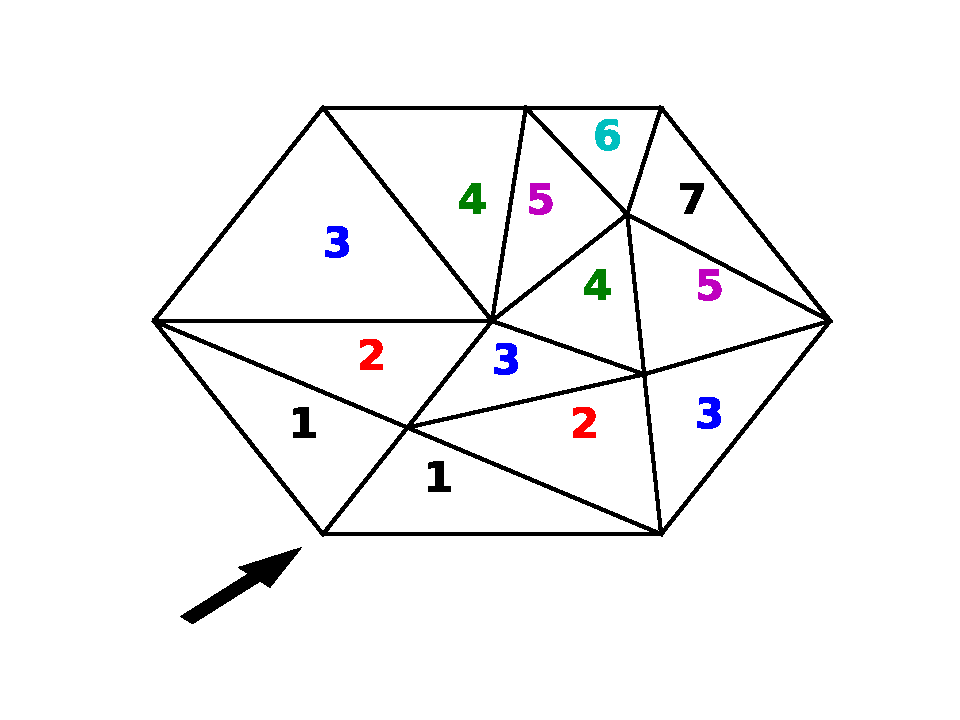
\includegraphics[scale=0.5]{../figures/UnstructuredMesh.pdf}
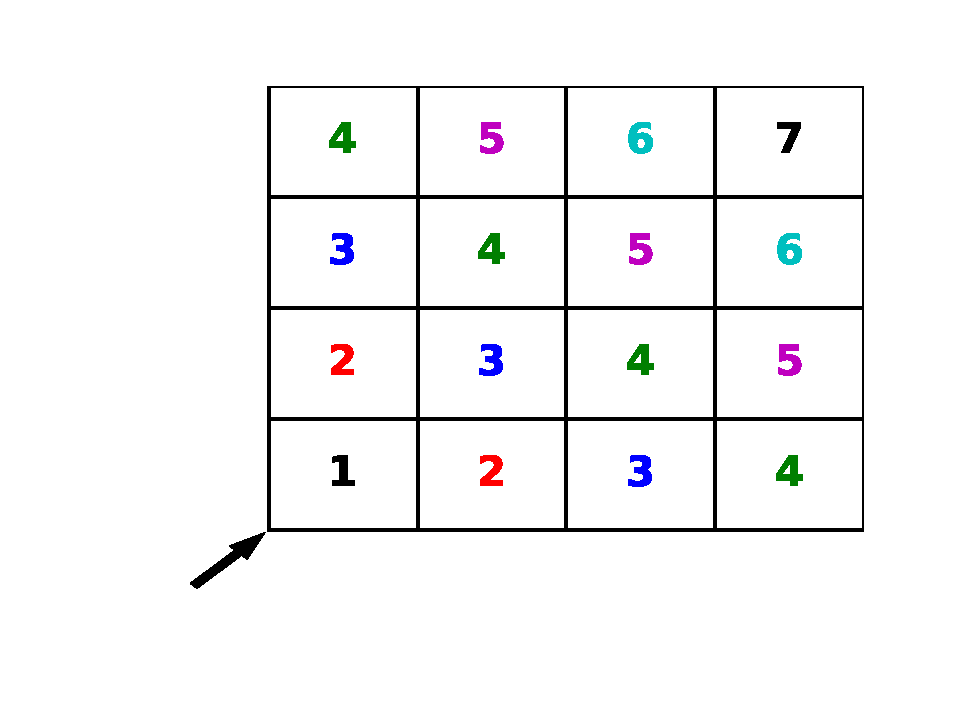
\includegraphics[scale = 0.5]{../figures/StructuredMesh.pdf}
\caption{A demonstration of a sweep on structured and unstructured meshes. }
\label{sweeps}
\end{figure}

The number in each cell represents the order in which the cells are solved.
Obtaining the solution for current cells in the sweep is dependent on the solution of downwind cells.
This process can be represented and stored as a task dependence graph, shown in Fig. \ref{tdg}.

\begin{figure}[H]
\centering
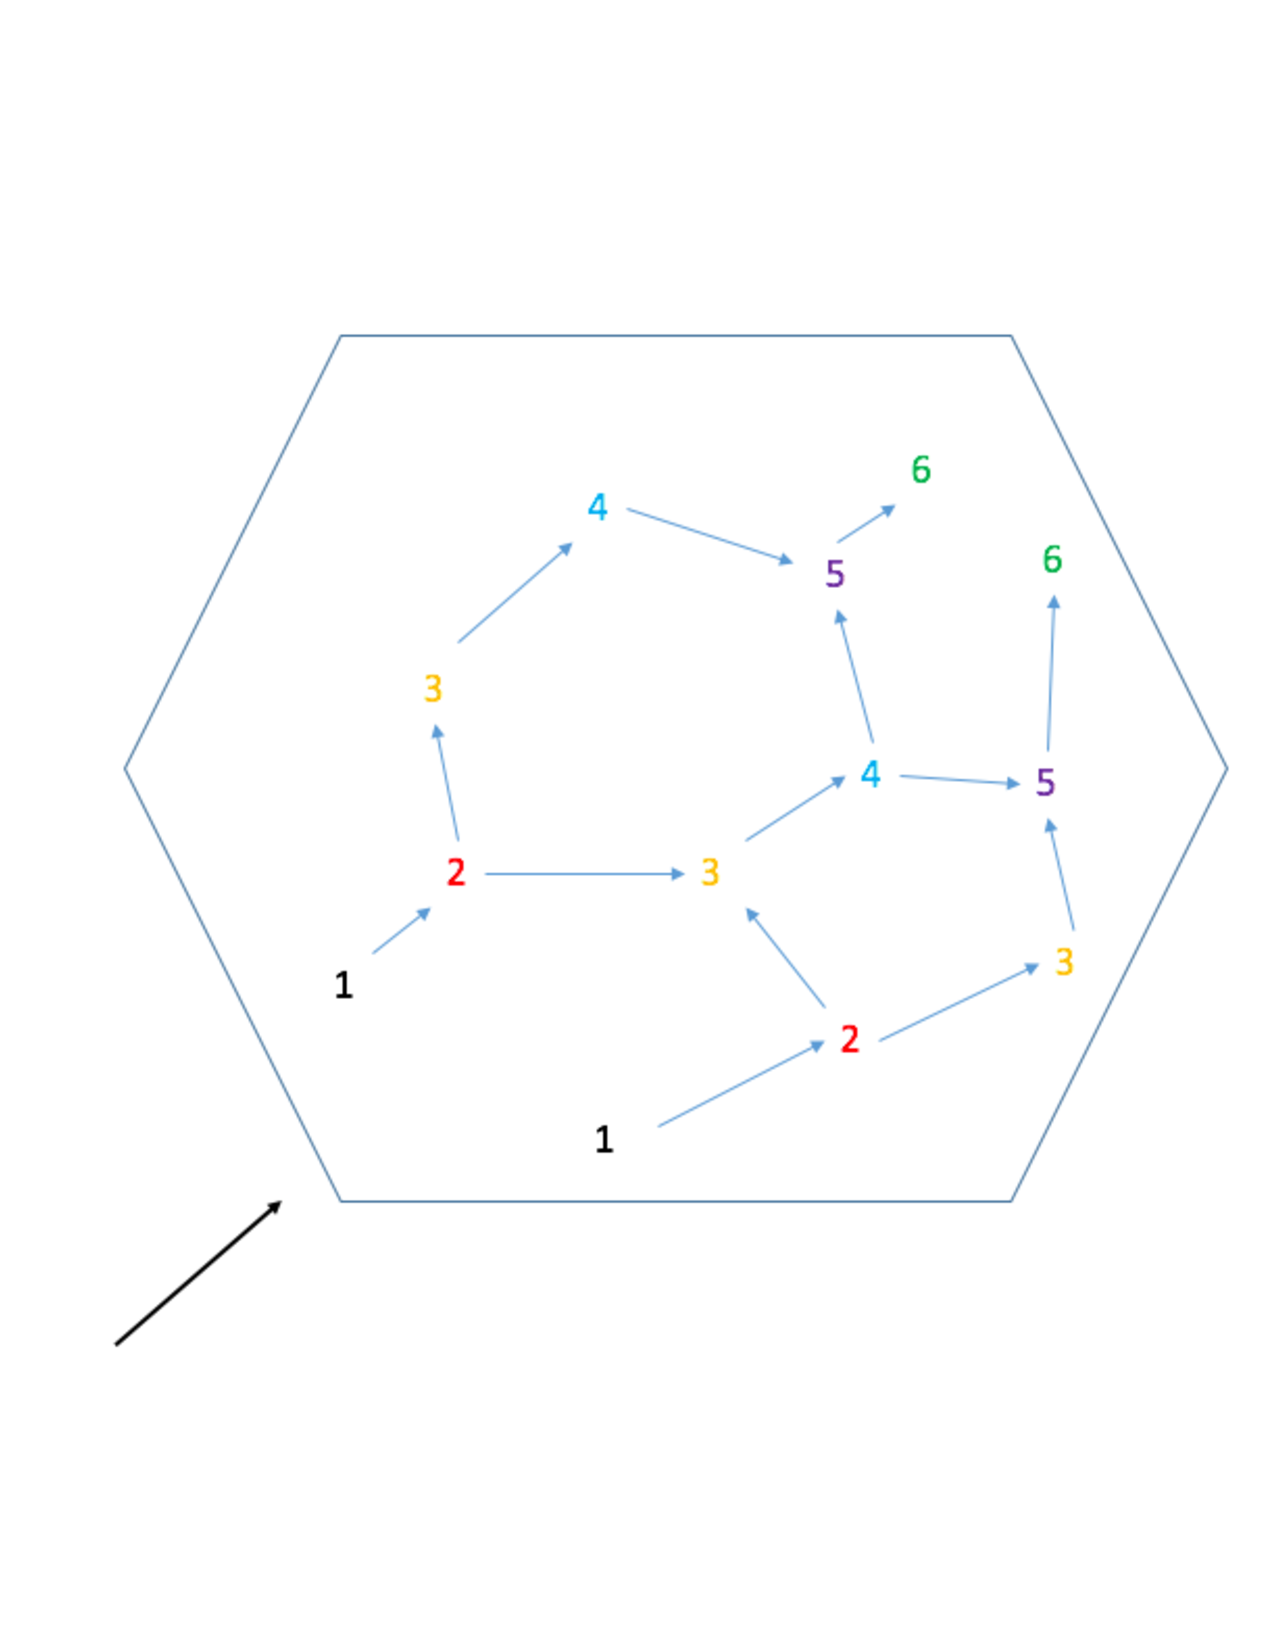
\includegraphics[scale = 0.35,trim={0cm 3cm 0cm 3cm},clip]{../figures/tdg.pdf}
\caption{A task dependence graph of the unstructured mesh example in Fig. \ref{sweeps}.}
\label{tdg}
\end{figure}

Massively parallel transport sweeps have been shown to scale up to 750,000 cores on logically Cartesian grids. However, structured meshes are somewhat limiting when  simulating more complex problems and experiments, requiring the use of unstructured meshes in transport sweeps. While unstructured meshes provide the ability to simulate realistic problems, they introduce some challenges like unbalanced partitions, which can increase the time to solution. To combat this, PDT, Texas A\&M University's massively parallel deterministic transport code, introduced two load balancing algorithms that rely on moving the spatial partition boundaries, or cut planes (cut lines in 2D), throughout the mesh in order to obtain a roughly equivalent amount of cells (and therefore work) per processor. However, this sacrifices the optimal partitioning scheme\cite{mpadams2013} in favor of balance. We propose a method that weighs ideal load balancing against the consequences to the transport sweep in order to achieve the best possible time to solution.



%%%%%%%%%%%%%%%%%%%%%%%%%%%%%%%%%%%%%%%%%%%%%%%%%%%
%
%  New template code for TAMU Theses and Dissertations starting Fall 2016.
%
%
%  Author: Sean Zachary Roberson
%  Version 3.17.09
%  Last Updated: 9/21/2017
%
%%%%%%%%%%%%%%%%%%%%%%%%%%%%%%%%%%%%%%%%%%%%%%%%%%%

%%%%%%%%%%%%%%%%%%%%%%%%%%%%%%%%%%%%%%%%%%%%%%%%%%%%%%%%%%%%%%%%%%%%%%%
%%%                           SECTION II
%%%%%%%%%%%%%%%%%%%%%%%%%%%%%%%%%%%%%%%%%%%%%%%%%%%%%%%%%%%%%%%%%%%%%%


\chapter{PARALLEL TRANSPORT SWEEPS}\label{cha:parallel_transport}
As mentioned in Chapter \ref{cha:transport_sweeps}, a transport sweep is set up by overlaying a domain with a finite element mesh and solving the transport equation cell by cell using a discontinuous finite element approach. A transport sweep can be solved in parallel in order to obtain the solution faster, as well as distribute the problem across many processors for memory intensive problems.

In PDT, a transport sweep can be performed on a structured Cartesian or arbitrary polyhedral mesh. Sweeping on an unstructured mesh presents two challenges: maintaining sweep efficiency on a massively parallel scale and keeping non-concave sub-domains to avoid cycles. PDT has already proven the ability to perform massively parallel transport sweeps on structured meshes. As part of previous efforts in PDT, researchers have outlined three important properties for parallel sweeps.

A parallel sweep algorithm is defined by three properties \cite{mpadams2013} :
\begin{itemize}
\item partitioning: dividing the domain among available processors,
\item aggregation: grouping cells, directions, and energy groups into tasks,
\item scheduling: choosing which task to execute if more than one is available.
\end{itemize}

The basic concepts of parallel transport sweeps, partitioning, aggregation, and scheduling, are most easily described in the context of a  transport sweep that takes place on a structured Cartesian mesh. Furthermore, the work detailed in Chapters \ref{cha:lb} and \ref{cha:tts} utilize aspects of the structured transport sweep.

In a regular grid, we have the  number of cells in each Cartesian direction: $N_x, N_y, N_z$. These cells are aggregated into ``cellsets'', using aggregation factors $A_x, A_y, A_z$. If $M$ is the number of angular directions per octant, $G$ is the total number of energy groups, and $N$ is the total number of cells, then the total fine-grain work units is $8MGN$. The factor of 8 is present as $M$ directions are swept for all 8 octants. We often discuss the directions in a sweep in terms of octant-pairs, or two octants that have opposing sweep ordering. This is an important concept that is discussed in Section \ref{sec:KBA}. The finest-grain work unit is the calculation of a single direction and energy group's unknowns in a single cell, or $\psi_{m,g}$ for a single cell.

Fine-grain work units are aggregated into coarser-grained units called \textit{tasks}. A few terms are defined that describe how each variable is aggregated.
\begin{itemize}
\item $A_x = \frac{N_x}{P_x}$, where $N_x$ is the number of cells in $x$ and $P_x$ is the number of processors in $x$.
\item $A_y = \frac{N_y}{P_y}$, where $N_y$ is the number of cells in $y$ and $P_y$ is the number of processors in $y$.
\item $A_z$ = a selectable number of z-planes of $A_x A_y$ cells.
\item $N_g = \frac{G}{A_g}$
\item $N_m = \frac{M}{A_m}$
\item $N_k = \frac{N_z}{P_z A_z}$
\item $N_k A_x A_y A_z = \frac{N_x N_y N_z}{P_x P_y P_z}$
\end{itemize}

It follows that each process owns $N_k$ cellsets (each of which is $A_z$ planes of $A_x A_y$ cells), $8N_m$ angle-sets, and $N_g$ group-sets for a total of $8N_m N_g N_k$ tasks.

One task contains $A_x A_y A_z$ cells, $A_m$ directions, and $A_g$ groups. Equivalently, a task is the computation of one cellset, one groupset, and one angleset, with the completion of one task defined as a stage.  The stage is particularly important when assessing sweeps against analytical performance models. 
Equation ~\eqref{paralleleff} defines parallel sweep efficiency:
\begin{equation}\label{paralleleff}
\begin{split}
\epsilon &= \frac{T_{\text{task}} N_{\text{tasks}}}{[N_{\text{stages}}] [T_{\text{task}} + T_{\text{comm}}]} \\
            &=\frac{1}{[1+\frac{N_{\text{idle}}}{N_{\text{tasks}}}][1 + \frac{T_{\text{comm}}}{T_{\text{task}}}]},
\end{split}
\end{equation}
where $N_\text{idle}$ is the number of idle stages per processor, $N_\text{tasks}$ is the number of tasks each processor performs, $T_\text{comm}$ is the time to communicate after completion of a task, and $T_\text{task}$ is the time it takes to compute one task.
Equations ~\eqref{Tcomm} and ~\eqref{Ttask} show how $T_{\text{comm}}$ and $T_{\text{task}}$ are calculated:
\begin{align}
T_{\text{comm}} &= M_L T_{\text{latency}} + T_{\text{byte}} N_{\text{bytes}}, \\
N_{\text{bytes}} &= (A_x A_y + A_x A_z + A_y A_z)A_g A_m upbc,
\label{Tcomm}
\end{align}
\begin{equation}
T_{\text{task}} = A_x A_y A_z A_m A_g T_{\text{grind}},
\label{Ttask}
\end{equation}
where $T_{\text{latency}}$ is the message latency time, $T_{\text{byte}}$ is the time required to send one byte of message, $N_{\text{bytes}}$ is the total number of bytes of information that a processor must communicate to its downstream neighbors at each stage, $upbc$ is the unknowns per boundary cell (generally 2 for 2D and 4 for 3D) and $T_{\text{grind}}$ is the time it takes to compute a single cell, direction, and energy group. $M_L$ is a latency parameter that is used to explore performance as a function of increased or decreased latency. Note that Eq. \ref{Ttask} is idealized as it does not take into account overhead in various parts of the sweep implementation.

Before expanding on the proposed method of partitioning and scheduling for parallel transport sweeps, a quick review of two parallel transport sweep algorithms is necessary. This dissertation's method will expand on PDT's sweep algorithm \cite{mpadams2013,mpadams2015}, which is an extension of the popular KBA algorithm \cite{KBA}.

\section{The KBA Algorithm}\label{sec:KBA}

Several parallel transport sweep codes use KBA partitioning in their sweeping, such as Denovo \cite{denovo} and PARTISN \cite{partisn}. The KBA partitioning scheme and algorithm was developed by Koch, Baker, and Alcouffe \cite{KBA}.

The KBA algorithm traditionally chooses $P_z = 1, A_m = 1 \text{ (or 1 angle per angleset)}, G = A_g = 1, A_x = N_x/P_x, A_y = N_y/P_y$, with $A_z$ being the selectable number of z-planes to be aggregated into each task. This partitions the domain into long, thin columns. With $N_k = N_z/A_z$, each processor performs $N_{\text{tasks}} = 8MN_k$ tasks. The KBA algorithm traditionally solves a problem one energy group at a time, and uses a ``pipelining'' or assembly line approach. This allows for new angles in an octant to begin sweeping before old angles have fully swept across the spatial domain. Figure \ref{pipeline_example} shows an example of pipelining the angular work of a quadrant.
Figure \ref{pipeline_example_3d} shows pipelining in the X-Z plane with $A_z = 1$. 

\begin{figure}[h]
\centering
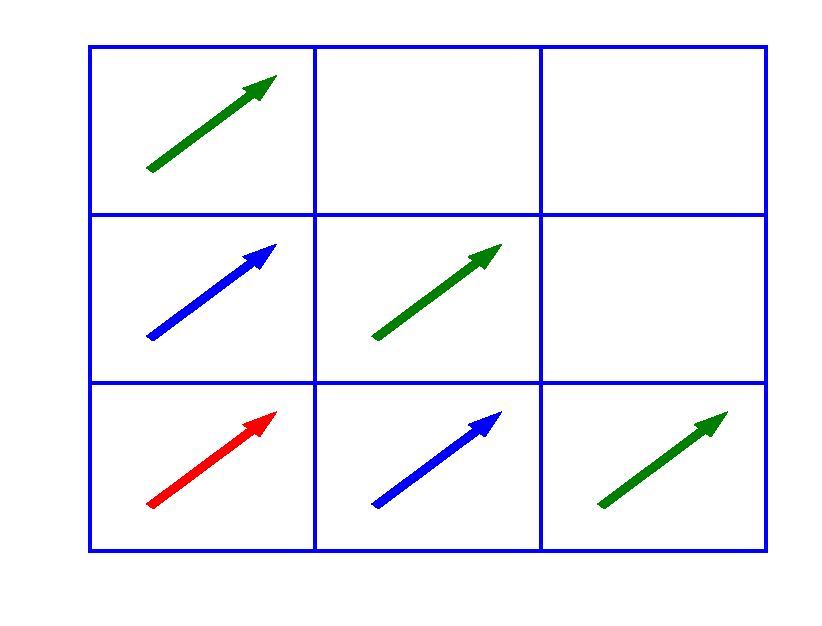
\includegraphics[scale=0.7]{../figures/pipeline_example.pdf}
\caption{An example showing the pipelining of angular work from the lower left quadrant.}
\label{pipeline_example}
\end{figure}
\begin{figure}[h]
\centering
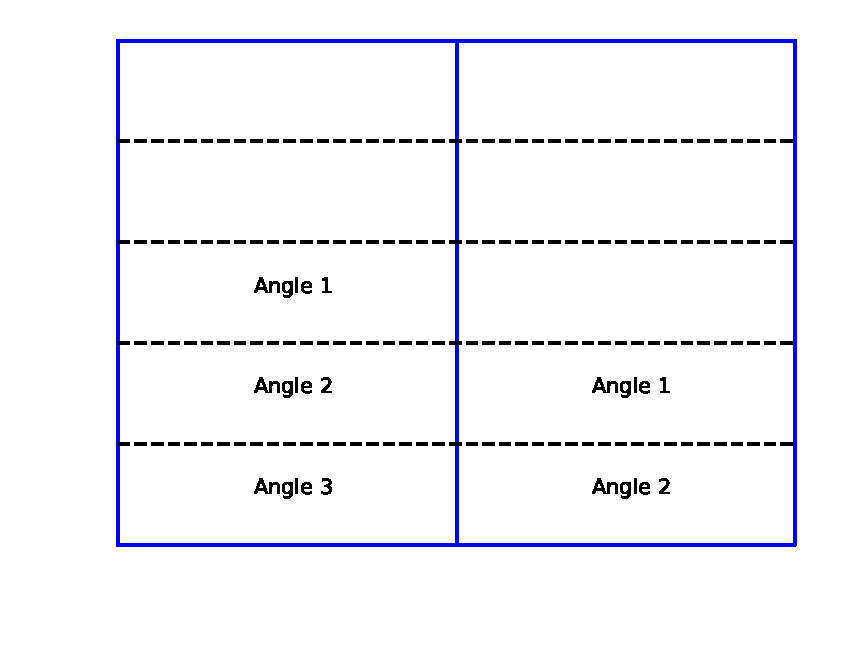
\includegraphics[scale=0.7,trim={0cm 1cm 0cm 0cm},clip]{../figures/pipeline_example_3d.pdf}
\caption{An example showing pipelining in the X-Z plane with $A_z = 1$, $P_x = 2$ and $P_z = 1$.}
\label{pipeline_example_3d}
\end{figure}

In Fig. \ref{pipeline_example}, each square represents a processor that owns a group of $A_xA_y$ cells. We see that as soon as a processor is free to solve the next angle with the same sweep ordering, it begins immediately.
Figure \ref{pipeline_example_3d} shows us the X-Z plane of a processor layout with $P_x = 2$ and $P_z = 1$. We see $N_k=\frac{N_z = 5}{A_z = 1}=5$ planes in Z, and three angles pipelined. We notice as soon as a cellset of $A_xA_yA_z$ cells is free to solve the next angle with the same sweep ordering, it begins immediately.
KBA introduced pipelining in order to combat the inherent inefficiencies of waiting for all processors to complete a sweep in a direction before starting the next angle.

There are two variants to the KBA algorithm, ``successive in angle, successive in quadrant", and ``simultaneous in angle, successive in quadrant".  With ``successive in angle, successive in quadrant", an octant pipelines its angular work, and once all directions are complete the opposing octant pipelines them back. This is then done for the remaining octant pairs. With ``simultaneous in angle, successive in quadrant", all angles from one octant are aggregated and solved rather than pipelined, and upon completion the opposing octant solves them. This is done either by aggregating angles, This is then done for the remaining octant pairs. The KBA parallel efficiency \cite{mpadams2013} for ``successive in angle, successive in quadrant" is:
\begin{equation}
  \epsilon_{KBA} = \frac{1}{[1 + \frac{4(P_x+P_y-2)}{8MN_k}][1 + \frac{T_{\text{comm}}}{T_{\text{{task}}}}]}.
  \label{eps_kba}
\end{equation}
The KBA parallel efficiency for ``simultaneous in angle, successive in quadrant'' is:
\begin{equation}
   \epsilon_{KBA} = \frac{1}{[1 + \frac{4(P_x+P_y-2)}{8MN_k/(A_m)}][1 + \frac{T_{\text{comm}}}{T_{\text{{task}}}}]}.
   \label{eps_kba_simul}
\end{equation}
For each octant-pair, the idle time is $P_x + P_y - 2$, and if the successive octant-pairs don't start until the previous octant pair finishes, then the total idle time is $4(P_x + P_y - 2)$. 

\section{PDT's Extension of KBA}\label {pdt_extension}

PDT's extension of KBA does not limit $P_z, A_m, G,$ or $A_g$. In addition, all 8 octants (4 quadrants in 2D) begin work immediately. Unlike KBA, PDT's scheduling requires conflict resolution in its algorithm, as the pipelines from all octants will end up colliding toward the middle of the processor domain.

If two or more tasks reach a processor at the same time, PDT employs a tie breaking strategy:

\begin{enumerate}
	\item The task with the greater depth-of-graph remaining (simply, more work remaining) goes first.
	\item If the depth-of-graph remaining is tied, then octant-priority tie-breaking is used:
	\begin{enumerate}
	  \item The task with $\Omega_x > 0$ wins.
	  \item If multiple tasks have $\Omega_x > 0$, then the task with $\Omega_y > 0$ wins.
	  \item If multiple tasks have $\Omega_y > 0$, then the task with $\Omega_z > 0$ wins.
	\end{enumerate}
\end{enumerate}

Given these conflict resolution techniques, the minimum possible number of stages for given partitioning parameters $P_i$ and $A_j$ is $2N_{\text{fill}} + N_{\text{tasks}}$. $N_{\text{fill}}$ is both the minimum number of stages before a sweepfront can reach the center-most processors and the number needed to finish a direction's sweep after the center-most processors have finished. Equations \ref{nfill}, \ref{nidle}, and \ref{ntasks} define $N_{\text{fill}}, N_{\text{idle}}$, and $N_{\text{tasks}}$:

\begin{align}
N_\text{fill} = \frac{P_x + \delta_x}{2} - 1 + \frac{P_y + \delta_y}{2} - 1 + N_k (\frac{P_z + \delta_z}{2} - 1)\label{nfill} \\ 
\delta_u = 0 \text{ or } 1 \text{ for $P_u$ even or odd, respectively} \nonumber
\end{align}
\begin{equation}
N_\text{idle} = 2N_{\text{fill}}
\label{nidle}
\end{equation}
\begin{equation}
N_\text{tasks} = 8N_mN_gN_k
\label{ntasks}
\end{equation}
Plugging these definitions into Eq. \ref{paralleleff}, the PDT optimal parallel efficiency \cite{mpadams2013} for $P_u$ even is:
\begin{equation}
	\epsilon_{opt} = \frac{1}{ [1 + \frac{P_x + P_y - 4 + N_k(P_z -2)}{8MGN_k/(A_m A_G)} ]  [ 1 +  \frac{T_{\text{comm}}}{T_{\text{task}}} ]}
	\label{eps_opt}
\end{equation}

Let's consider how many more processors the hybrid partitioning with optimal scheduling ($P_z = 2$) can use while yielding the same efficiency as KBA.
Let's consider the limit of a large number of processors for both KBA and hybrid partioning with an optimal schedule.
Equation \ref{large_p_kba} shows the KBA efficiency in the large-P limit with $P_x + P_y \approx 2P^{1/2}$.
Setting $A_m = A_g = 1$ to match traditional KBA aggregation parameters, Eq. \ref{large_p_opt} shows the hybrid optimal efficiency in the large-P limit with $P_z = 2$ and $P_x + P_y \approx 2P^{1/2}$.  
\begin{equation}
  \epsilon_{KBA} \xrightarrow{\text{large P}} \frac{1}{[1 + \frac{(4P^{1/2})}{8MN_k}][ 1 +  \frac{T_{\text{comm}}}{T_{\text{task}}}]}
  \label{large_p_kba}
\end{equation}
\begin{equation}
  \epsilon_{opt,hybrid} \xrightarrow{\text{large P}} \frac{1}{[1 + \frac{\sqrt{2}P^{1/2}}{8MN_k}][ 1 +  \frac{T_{\text{comm}}}{T_{\text{task}}} ]}
  \label{large_p_opt}
\end{equation}

If we set Eq. \ref{large_p_kba} equal to Eq. \ref{large_p_opt}, we see that in the limit of a large number of processors $P$, the optimal algorithm yields the same efficiency as KBA with 32 times as many processors \cite{mpadams2013, mpadams2015}.

\section{PDT's Performance Model}

To aid in the selection of optimal processor and aggregation parameters, PDT uses a performance model to estimate the sweep time.
This performance model is the basis for the cost function described in Chapter \ref{cha:tts}.
Equation \ref{sweep_time} calculates the sweep time by multiplying the time it takes to solve each stage by the number of stages. This is then multiplied by a multi-core fudge factor that estimates the performance drop-off from 1 to 8 cores.
\begin{equation}
\text{Sweep Time} = \text{mcff}\cdot[\text{num stages}\cdot(T_{wu} + 3\cdot \text{latency}\cdot M_L + T_{\text{byte}}\cdot N_{\text{bytes}} + N_{\text{cells}}\cdot ( T_c +  A_m\cdot (T_m + T_g)))],
\label{sweep_time}
\end{equation}
where:
\begin{itemize}
  \item mcff = the Multi-Core Fudge Factor, a corrective factor that accounts for performance drop-off from 1 to 8 cores,
  \item num stages = tasks per processor + $2N_{\text{idle}}$,
  \item tasks per processor = $\frac{N_x}{P_x A_x} \frac{N_y}{P_y A_y} \frac{N_z}{P_z A_z} \frac{N_m}{A_m} \frac{N_g}{A_g}$,
  \item $T_{wu}$ = the time to get into the sweep operator,
  \item latency = the machine specific communication latency,
  \item $M_L$ = the machine specific latency multiplier,
  \item $T_{\text{byte}}$ = the communication time per double,
  \item $N_{\text{byte}}$ = the bytes per 3 communications (assuming 3 neighbors) = $(A_x A_y + A_x A_z + A_y A_z)A_g A_m upbc $,
  \item $upbc$ = unknowns per boundary cell (4 for 3d, 2 for 2d),
  \item $N_{\text{cells}}$ = the number of cells per task, $A_x A_y A_z$,
  \item $T_c$ = the time spent solving cell-specific work,
  \item $T_m$ = the time spent solving angle-specific work,
  \item $T_g$ = the time spent solving group-specific work.
\end{itemize}

A comparison between this performance model and the time-to-solution estimator will be shown in Chapter \ref{cha:tts}. Before this, we motivate the need for the time-to-solution estimator in Chapter \ref{cha:lb} by describing unstructured meshes in PDT and how we load balance them.

%%%%%%%%%%%%%%%%%%%%%%%%%%%%%%%%%%%%%%%%%%%%%%%%%%%
%
%  New template code for TAMU Theses and Dissertations starting Fall 2016.  
%
%
%  Author: Sean Zachary Roberson
%  Version 3.17.09
%  Last Updated: 9/21/2017
%
%%%%%%%%%%%%%%%%%%%%%%%%%%%%%%%%%%%%%%%%%%%%%%%%%%%
%%%%%%%%%%%%%%%%%%%%%%%%%%%%%%%%%%%%%%%%%%%%%%%%%%%%%%%%%%%%%%%%%%%%%%
%%                           SECTION III
%%%%%%%%%%%%%%%%%%%%%%%%%%%%%%%%%%%%%%%%%%%%%%%%%%%%%%%%%%%%%%%%%%%%%

\chapter{UNSTRUCTURED MESHING AND LOAD BALANCING IN PDT}\label{cha:lb}

Initially, PDT only swept on structured, logically Cartesian meshes. As the need to solve problems with more complex geometries arose, PDT added a support for arbitrary polyhedral unstructured meshes. However, this introduced imbalanced partitions (or different amounts of cells per processor), causing longer and unmanageable runtimes.

To combat imbalanced partitions, two load balancing algorithms were implemented, referred to in this thesis as the original load-balancing algorithm \cite{mastersthesis,mc2017} and the load-balancing-by-dimension algorithm.

Before detailing the two load balancing algorithms PDT employs, a quick review of partitioning unstructured meshes in PDT is necessary:
\begin{itemize}
\item ``Cut lines'' in 2D (``cut planes'' in 3D) are used to slice through the mesh in the $x$, $y$, and $z$ dimensions.
\item The cut planes form brick partitions, called subsets, that have unstructured meshes inside of them. 
\item Discontinuities along subset boundaries are fixed by ``stitching'' hanging nodes, creating degenerate polygons along subset boundaries.
\item The subsets are distributed amongst the processor domain.
\end{itemize}
Using cut lines/cut planes to partition unstructured meshes preserved the provably optimal sweep partitioning \cite{mpadams2013,mpadams2015} of logically Cartesian grids. 
Subsets, rather than the cells, have $(i,j,k)$ indices and will become the base unit when aggregating spatial parameters. That is, $A_x$ and $A_y$ will now represent the number of subsets in $x$ and $y$ aggregated into a task. 
Figure \ref{partitioning_example} shows an example of an unstructured mesh partitioned into 100 subsets in PDT. 
\begin{figure}[H]
\centering
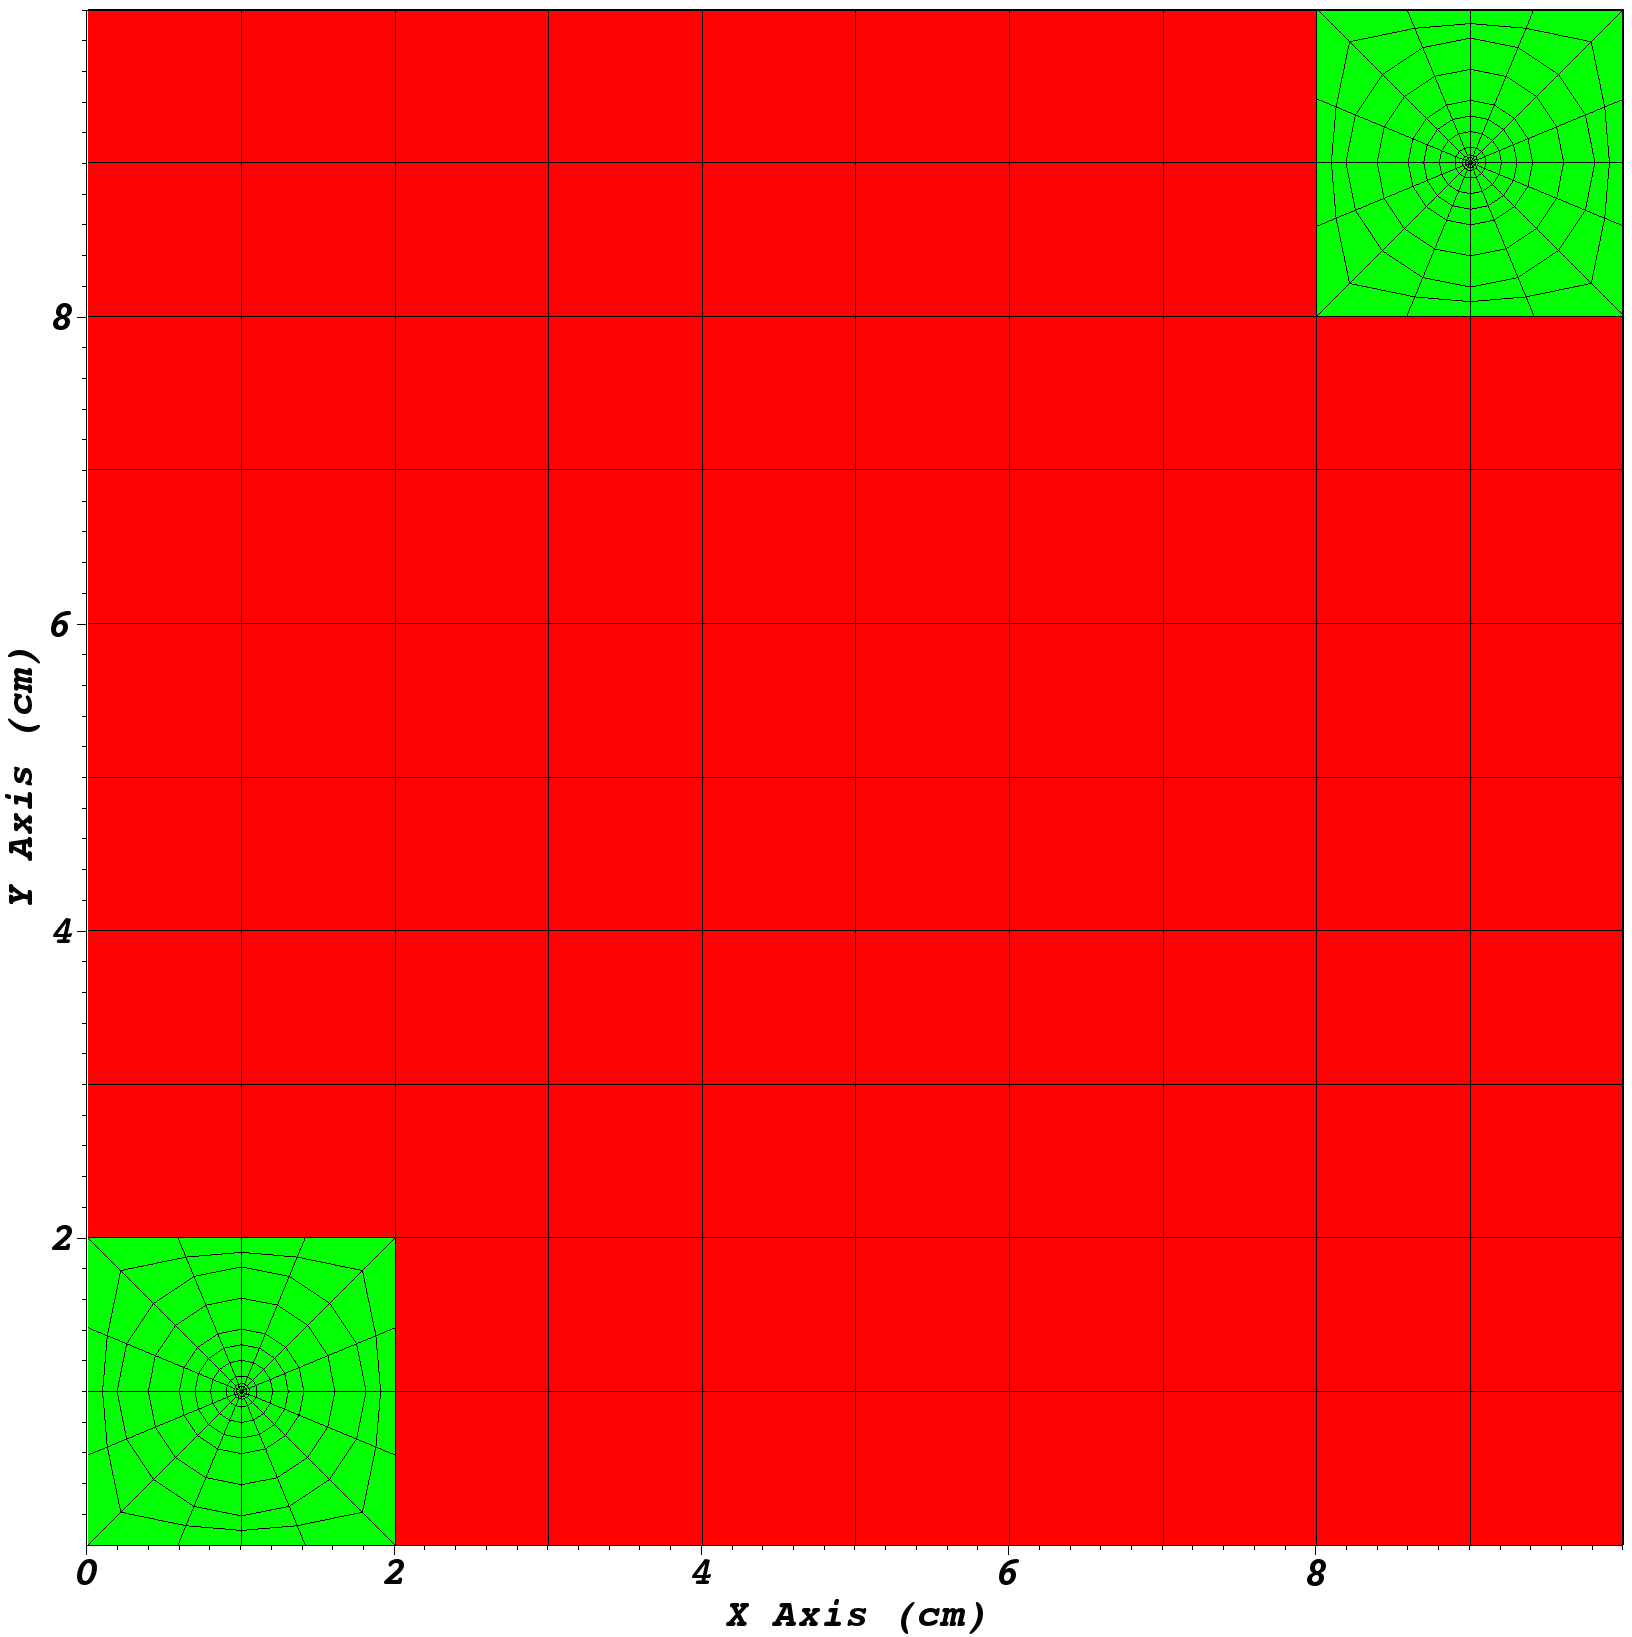
\includegraphics[scale=0.2]{../figures/spiderweb_10x10_sparse.png}
\caption{An unstructured mesh partitioned into 100 subsets with cut lines at 1 cm intervals in both dimensions}
\label{partitioning_example}
\end{figure}

Upon creation, the subsets may have geometric discontinuities as a result of slicing through the mesh. 
Figure \ref{hanging_node} shows an example of a hanging node across a subset boundary. 
This node is stitched across the boundary to preserve geometric continuity, forming a degenerate polygon \cite{degenerate} (in Fig. \ref{hanging_node}, a degenerate square). 
PDT uses Piece-Wise Linear Discontinuous (PWLD) finite-element basis functions \cite{pwld_ragusa,pwld_teresa} that allow for solutions on arbitrary and degenerate polyhedra. 
\begin{figure}[H]
  \centering
  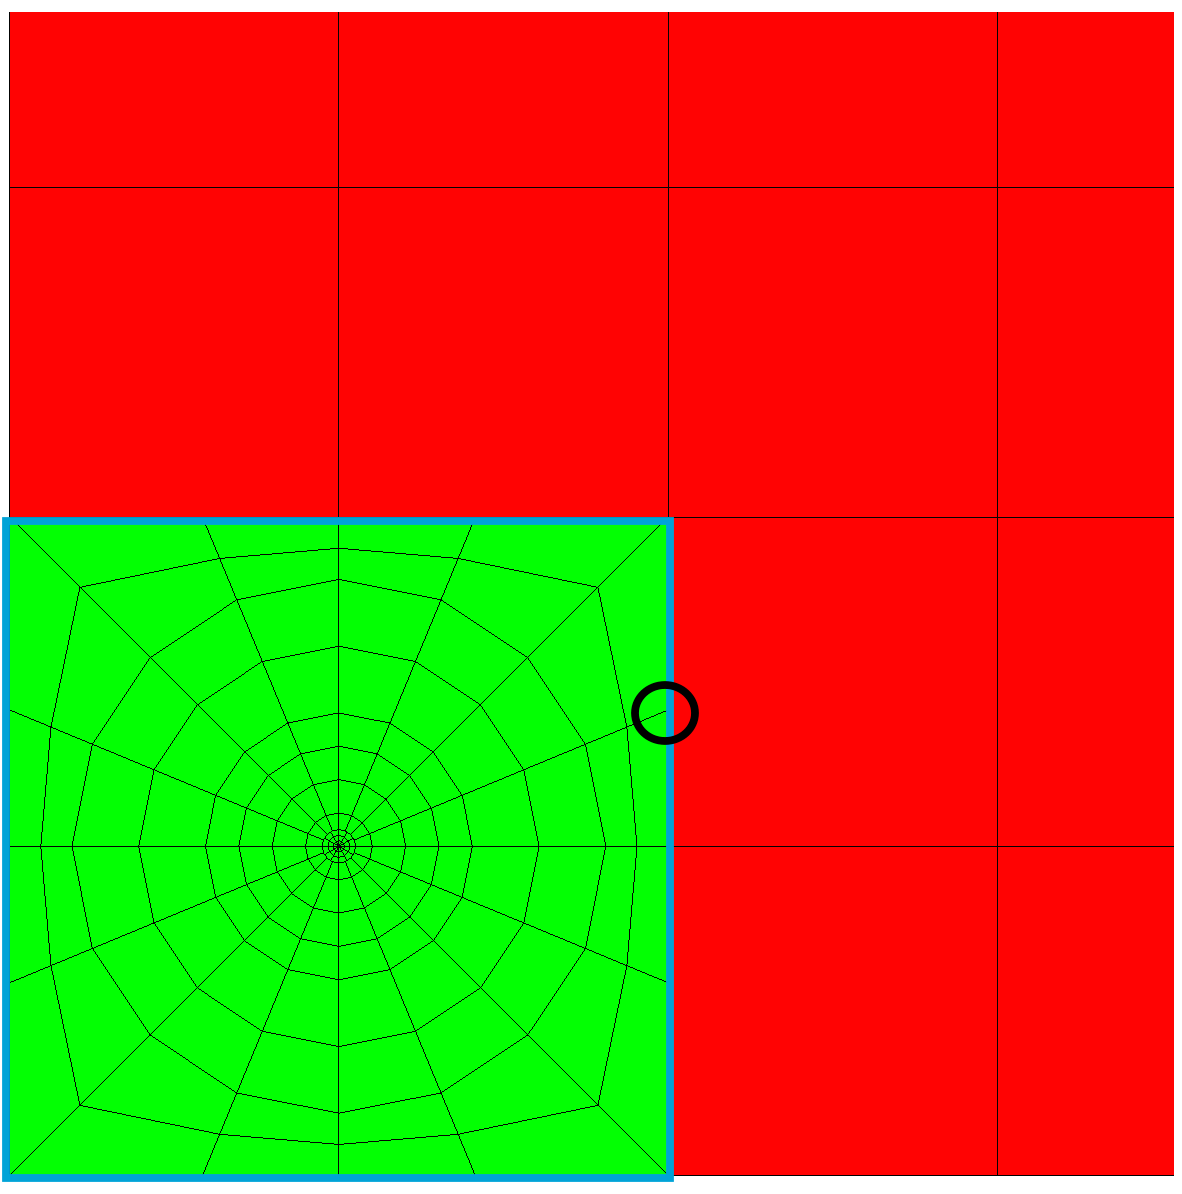
\includegraphics[scale=0.2]{../../figures/hanging_node_spiderweb_example.png}
   \caption{A hanging node (circled in black) on a subset boundary (highlighted in blue).}
   \label{hanging_node}
\end{figure}

Both approaches to load balancing move cut lines in order to redistribute cells more evenly throughout subsets. We define a metric describing how imbalanced our problem is:
\begin{equation}
f =\frac{\underset{ijk}{\text{max}}(N_{ijk})}{\frac{N_{tot}}{I\cdot J\cdot K}},
\label{metric_def}
\end{equation}
where $f$ is the load balance metric, $N_{ijk}$ is the number of cells in subset $(i,j,k)$, $N_{tot}$ is the global number of cells in the problem, and $I$, $J$, and $K$ are the total number of subsets in the $x$, $y$, and $z$ directions, respectively. The metric is a measure of the maximum number of cells per subset divided by the average number of cells per subset. For a perfectly balanced problem, $f = 1$.

Figure \ref{redistribute} illustrates an example of redistributing the cut planes in $x$ to balance the cells per column.
\begin{figure}[H]
\centering
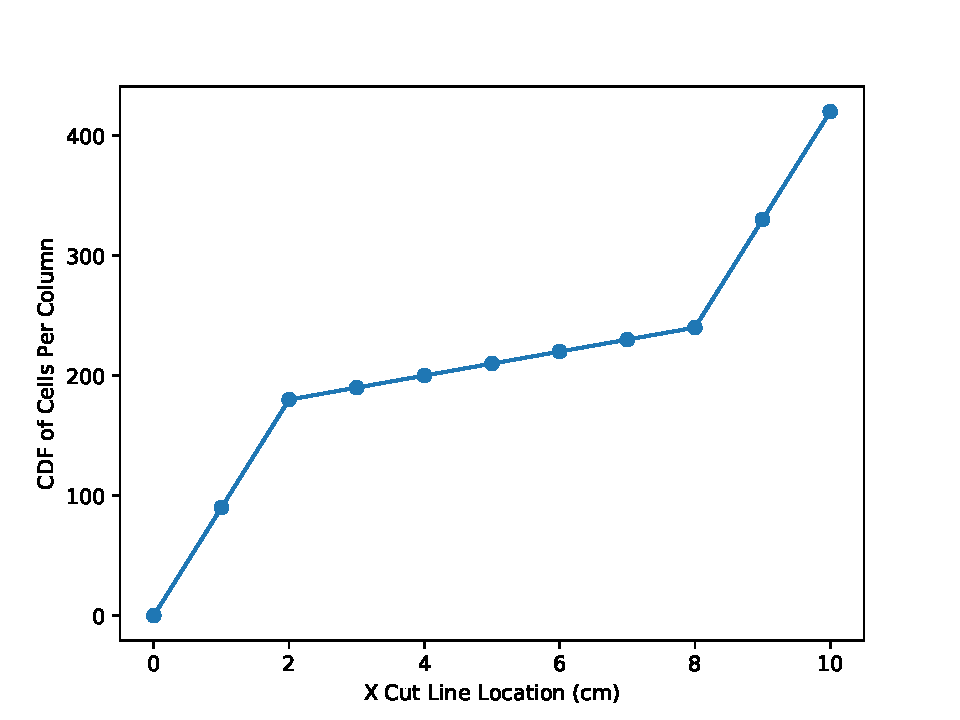
\includegraphics[scale=0.4]{../figures/spiderweb_redistribute_before_sparse.pdf}
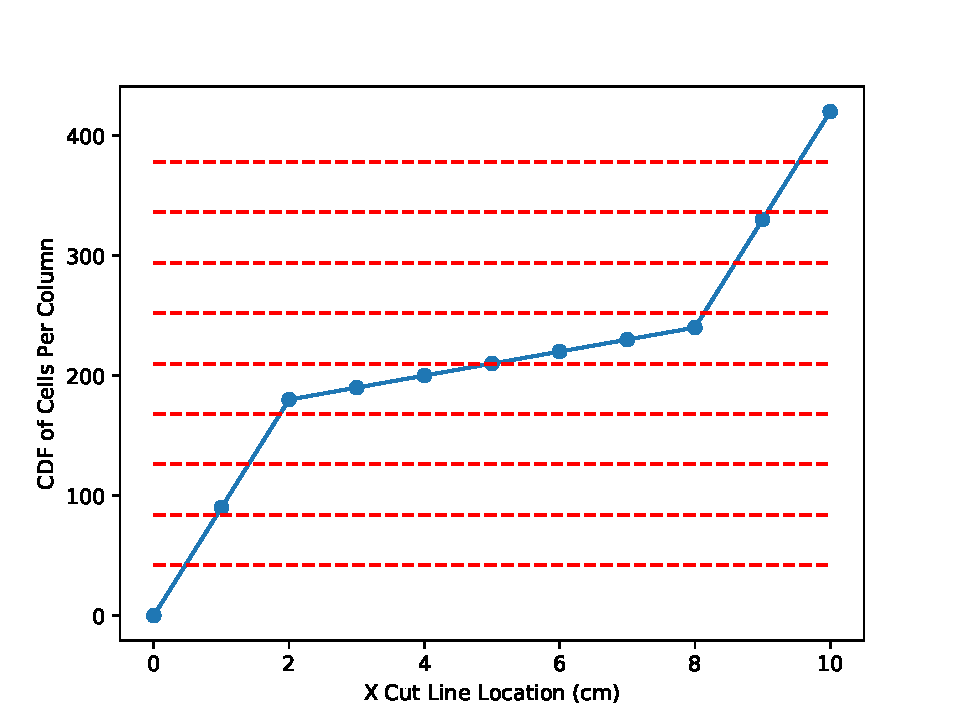
\includegraphics[scale=0.4]{../figures/spiderweb_redistribute_after_sparse.pdf}
\caption{The use of the CDF of cells per column to redistribute the cut lines in X.}
\label{redistribute}
\end{figure}
The image on the left side of Fig. \ref{redistribute} shows the CDF of the cells per column in Fig. \ref{partitioning_example}. The red lines on the right side of Fig. \ref{redistribute} show the ideal equal number of cells per column. The x-value of the intersection of these red lines and the CDF are where the cut lines are redistributed to. 

In order to decide the necessity of redistributing a dimension's cut lines/planes, we use dimensional sub-metrics of the following form:
\begin{equation}
f_{Z} = \frac{\underset{k}{\text{max}}[\sum_{i,j} N_{ijk}]}{\frac{N_{tot}}{K}},
\label{f_z}
\end{equation}
where $K$ is the total number of z-planes. 
Equation \ref{f_z} is a metric defining how imbalanced the problem's planes are. It calculates the maximum cells per plane divided by the average cells per plane. If $f_K$ is greater than a predefined tolerance, the z cut planes are redistributed using the process in Fig. \ref{redistribute}. 
 
\section{Original Load-Balancing Algorithm}
\label{sec:og_lb}

The initial approach to load balancing was implemented on 2D extruded meshes, meaning the mesh is balanced in the 2D plane and then extruded, yielding a balanced 3D mesh. The metrics for this algorithm are defined as follows:
\begin{align}
f &= \frac{\underset{ij}{\text{max}}(N_{ij})}{\frac{N_{tot}}{I\cdot J}}  \label{og_metric}\\
f_X &= \frac{\underset{i}{\text{max}}[\sum_{j} N_{ij}] } {\frac{N_{tot}}{I}} \label{og_i_metric} \\
f_Y &= \frac{\underset{j}{\text{max}}[\sum_{i} N_{ij}] } {\frac{N_{tot}}{J}} \label{og_j_metric}
\end{align}
Equation \ref{og_metric} mirrors Eq. \ref{metric_def} for 2 dimensions, and Eqs. \ref{og_i_metric} and \ref{og_j_metric} define the column and row-wise metrics respectively. 

 Algorithm \ref{initial_algorithm} summarizes the original approach to load balancing meshes in PDT.
\begin{algorithm}[H]
\caption{The original load-balancing algorithm.}
\label{initial_algorithm}
\begin{algorithmic}

\WHILE{$f > 1 + \text{tol}_{\text{subset}}$}
  \IF {$f_X > 1 + \text{tol}_{\text{col}}$}
    \STATE Redistribute the X cut lines.
  \ENDIF
  \IF {$f_Y > 1 + \text{tol}_{\text{row}}$}
  	\STATE Redistribute the Y cut lines.
  \ENDIF
\ENDWHILE
\end{algorithmic}
\end{algorithm}
While the problem is not balanced:
\begin{itemize}
  \item Check if the columns are balanced, and if not redistribute the X cut lines.
  \item Check if the rows are balanced, and if not redistribute the Y cut lines.
  \item Repeat until the mesh is balanced or until a maximum number of iterations is reached.
\end{itemize}

The original load-balancing algorithm placed cut lines in all dimensions all the way through the mesh. 
This created an orthogonal partitioning where each subset had an equivalent number of neighbors, which was done to preserve the provably optimal sweep partitioning described by Adams et. al \cite{mpadams2013,mpadams2015}. 
However, there are theoretical limits to load balancing in this fashion. Figure \ref{2dgeneral} shows a simple 2D subset layout with $M$ unaligned patches with $N$ cells each.

\begin{figure}[H]
\centering
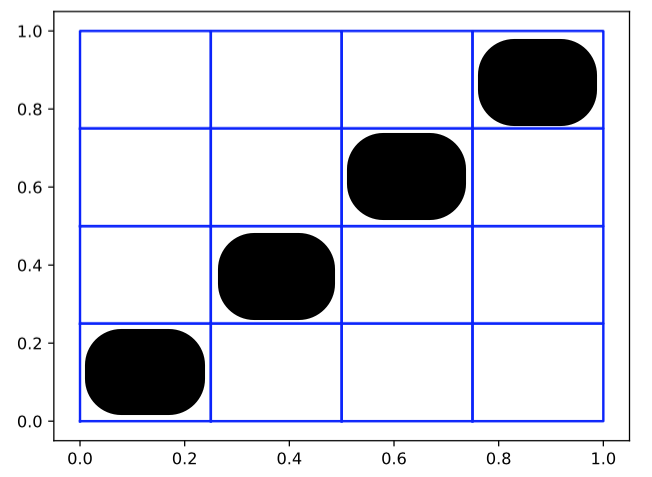
\includegraphics[scale=0.4]{../figures/theoretical_plot.png}
 \caption{A 2D subset layout with $M$ unaligned patches of high mesh density $N$.}
\label{2dgeneral}
\end{figure}
The subset layout is $M^2$, but only $M$ subset have significant work, leading to a theoretical limit for the load imbalance factor:
\begin{equation}
f= \frac{N}{(MN+C)/M^2} \xrightarrow{N\to \infty} \frac{N}{N/M} = M.
\end{equation}
Due to this theoretical limit, the load-balancing-by-dimension algorithm was developed.

\section{Load-Balancing-by-Dimension Algorithm}
\label{sec:lbd}

The load-balancing-by-dimension by dimension (LBD) algorithm, similar to the original load-balancing algorithm, relies on the movement of cut lines/planes to redistribute mesh cells in a more balanced manner.
However, cut lines are no longer required to go all the way through the mesh, and the load-balancing-by-dimension algorithm is fully extensible to 3 dimensions. 
The load-balancing-by-dimension algorithm is summarized by:
\begin{enumerate}
  \item Slice the mesh in $z$ and redistribute cut planes until each plane has approximately an equivalent number of cells.
  \item For each $z$ layer, slice the layer in columns and redistribute the $x$ cut lines until each column has an approximately equivalent number of cells.
  \item For each column within each $z$ layer, slice the column in rows and redistribute the $y$ cut lines until each row has an approximately equivalent number of cells.
\end{enumerate}

We once again use dimensional sub-metrics to determine whether or not a dimension's cut lines/planes need to be redistributed. The $z$ dimension's sub-metric is defined by Eq. \ref{f_z}. For the LBD algorithm, there are $K$ column-wise metrics, one for each $z$ layer:
\begin{equation}
f_{X,k} = \frac{ \underset{i}{\text{max}}[ \sum_{j} N_{ijk}]  }  {\frac{N_{tot,k}}{I}}.
\label{lbd_x_metric}
\end{equation}
Equation \ref{lbd_x_metric} defines the column-wise metric for layer $k$, or the maximum number of cells per column in layer $k$ divided by the average number of cells per column in layer $k$. 

For the LBD algorithm, there are $K\cdot I$ row-wise metrics, one for each column in each $z$ layer:
\begin{equation}
f_{Y,k,i} = \frac{\underset{j}{\text{max}} N_{ijk} } {\frac{N_{tot,k,i}}{J}}.
\label{lbd_y_metric}
\end{equation}
Equation \ref{lbd_y_metric} defines the row-wise metric for layer $k$ in column $i$, or the maximum number of cells per row in column $i$ in layer $k$ divided by the average number of cells per row in column $i$ in layer $k$. 

Algorithm \ref{lbd} details the load-balancing-by-dimension algorithm. 
\begin{algorithm}[H]
\caption{The load-balancing-by-dimension algorithm.}
\label{lbd}
\begin{algorithmic}

  \WHILE {$f_{Z} > 1 + \text{tol}_{\text{K}}$}
    \STATE Redistribute the Z cut planes.
  \ENDWHILE  
  
  \FOR {$k$ in $K$}
    \WHILE {$f_{X,k} > 1 + \text{tol}_{\text{I}}$}
      \STATE Redistribute the X cut lines within layer $k$. 
    \ENDWHILE
  \ENDFOR
  
  \FOR{$k$ in $K$}
    \FOR{$i$ in $I$}
      \WHILE {$f_{Y,k,i} > 1 +  \text{tol}_{\text{J}}$ }
        \STATE Redistribute the Y cut lines in column $i$ in layer $k$. 
      \ENDWHILE
    \ENDFOR
  \ENDFOR
  
  \STATE Calculate $f$.
\end{algorithmic}
\end{algorithm}

Figure \ref{alg_illustration} illustrates the behavior of both algorithms. In the left image of the figure, we see the partitions cutting across the entire domain, with the left-most $x$ cut line moved into the denser geometric feature in the bottom left corner to more evenly distribute cells. In the right image of the figure, we see the $x$ partitions cutting across the entire domain, but the $y$ partitions being redistributed by column. The $y$ partitions are moved into the respective geometric features in the appropriate columns in order to better balance the problem.

\begin{figure}[H]
\centering
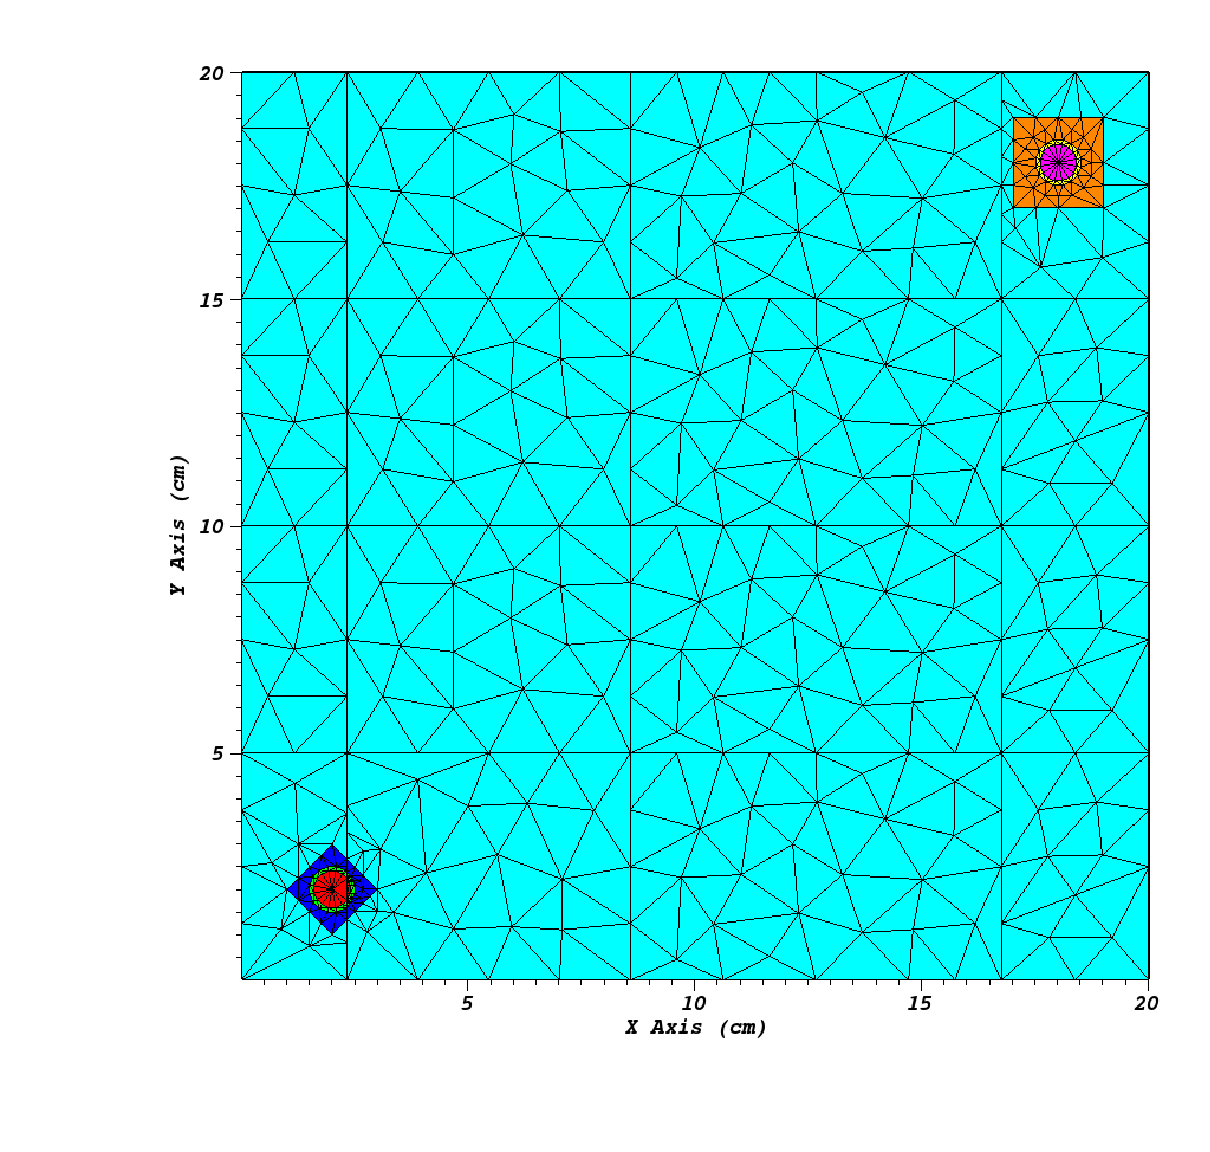
\includegraphics[scale=0.45,trim={0.95in 0.64in 0.35in 0.44in},clip]{../figures/og_lb_example.pdf}
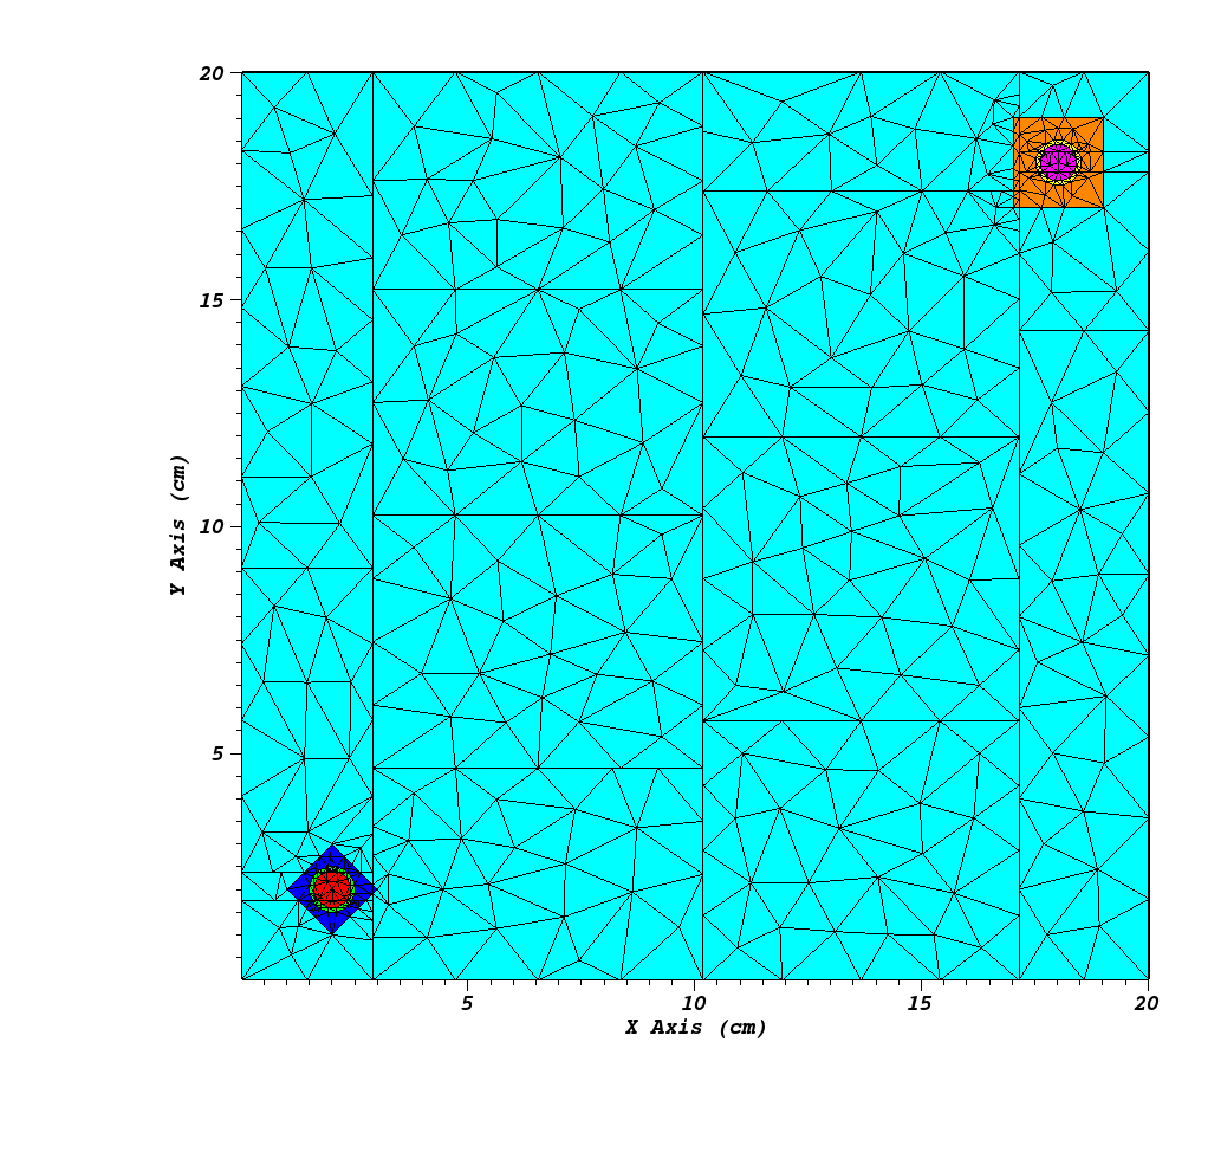
\includegraphics[scale=0.45,trim={0.95in 0.64in 0.35in 0.44in},clip]{../figures/lbd_example.pdf}
\caption{The partitions of a problem after the original load balancing (left) and the load-balancing-by-dimension (right) algorithms.}
\label{alg_illustration}
\end{figure}


\section{Results}

To show the behavior of the original load balancing algorithm and the load-balancing-by-dimension algorithm, the problem shown in Fig. \ref{partitioning_example} was run with a varying number of subsets and with a varying maximum triangle area, with the minimum allowable angle per triangle was kept constant at \ang{20}. We varied the number of subsets in $x$ and $y$ from 2 to 10 (with the total number of subsets varying from 4 to 100). The problem illustrated by Fig. \ref{partitioning_example} was chosen because it has two dense features in opposing corners with no features in between, lending itself to being an imbalanced mesh. Table \ref{og_table} shows the results of this parametric study using the original load balancing algorithm vs. using the load-balancing-by-dimension algorithm. Table \ref{all_improvements} shows the percent improvements for both algorithms from no load balancing to running both load balancing algorithm, while Table \ref{method_improvement} shows the improvement of the load-balancing-by-dimension algorithm relative to the original load balancing algorithm.

%\vspace{-1cm}
\begin{table}[H]
\centering
  \caption{\bf The results of the parametric study using the original load balancing algorithm (left) and the load-balancing-by-dimension algorithm (right).}
  \scalebox{0.5}{
  \begin{tabular}{c|c|c|c|c|c|c|c|c|c} 
  \bf Area, $N^{1/2}$ & \bf  2 &  \bf 3    &  \bf  4   &  \bf  5   &  \bf  6   &  \bf  7   & \bf   8   &  \bf 9    &  \bf 10   \\ \hline \hline
\bf Coarse&1.993 & 2.735 & 4.360 & 4.812 & 5.545 & 6.321 & 3.114 & 2.697 & 1.893 \\ \hline 
\bf 1.8& 1.408 & 2.277 & 2.886 & 3.269 & 4.716 & 4.721 & 5.890 & 4.618 & 1.863 \\ \hline
\bf 1.6& 1.375 & 2.206 & 2.649 & 3.247 & 4.356 & 4.876 & 4.678 & 5.062 & 1.329 \\ \hline
\bf 1.4& 1.337 & 2.110 & 2.982 & 3.031 & 4.615 & 4.310 & 8.911 & 4.652 & 2.675 \\ \hline
\bf 1.2& 1.344 & 2.008 & 2.017 & 3.392 & 3.916 & 4.969 & \cellcolor{blue!25}9.576 & 4.543 & 4.728 \\ \hline
\bf 1.0& 1.264 & 1.806 & 2.405 & 2.976 & 3.657 & 4.317 & 6.242 & 4.831 & 4.941 \\ \hline
\bf 0.8& 1.212 & 1.640 & 2.300 & 2.436 & 2.941 & 4.395 & 7.420 & 4.466 & 3.947 \\ \hline
\bf 0.6& 1.153 & 1.567 & 2.045 & 2.368 & 3.199 & 2.999 & 7.206 & 4.101 & 3.592 \\ \hline
\bf 0.4& 1.108 & 1.411 & 1.633 & 2.117 & 2.383 & 2.646 & 6.970 & 3.086 & 2.511 \\ \hline
\bf 0.2& 1.052 & 1.197 & 1.258 & 1.523 & 1.789 & 1.857 & 3.380 & 2.193 & 1.883 \\ \hline
\bf 0.1& 1.029 & 1.092 & 1.149 & 1.207 & 1.276 & 1.420 & 2.015 & 1.565 & 1.247 \\ \hline
\bf 0.08& 1.009 & 1.043 & 1.086 & 1.101 & 1.179 & 1.267 & 2.118 & 1.551 & 1.271 \\ \hline
\bf 0.06& 1.009 & 1.024 & 1.059 & 1.094 & 1.138 & 1.154 & 1.825 & 1.432 & 1.138 \\ \hline
\bf 0.05& 1.008 & 1.023 & 1.025 & 1.028 & 1.073 & 1.149 & 1.666 & 1.380 & 1.110 \\ \hline
\bf 0.04& 1.005 & 1.016 & 1.017 & 1.021 & 1.038 & 1.051 & 1.520 & 1.311 & 1.080 \\ \hline
\bf 0.03& 1.005 & 1.008 & 1.018 & 1.039 & 1.059 & 1.073 & 1.450 & 1.179 & \cellcolor{red!25}1.001 \\ \hline
\bf 0.02& 1.005 & 1.008 & 1.010 & 1.013 & 1.021 & 1.035 & 1.623 & 1.137 & 1.016 \\ \hline
\bf 0.01& 1.003 & 1.009 & 1.009 & 1.011 & 1.016 & 1.013 & 1.281 & 1.058 & 1.015 \\ \hline
  \end{tabular}}
 \scalebox {0.5}{
   \begin{tabular}{c|c|c|c|c|c|c|c|c|c} 
\bf Area, $N^{1/2}$ & \bf  2 & \bf 3    &  \bf  4   &  \bf  5   &  \bf 6    &  \bf  7   &   \bf 8   &  \bf 9    &  \bf 10   \\ \hline \hline
\bf Coarse & 1.645 & 1.455 & 1.878 & 2.348 & 3.046 & 3.022 & 1.752 & 2.304 & 1.451 \\ \hline 
\bf 1.8& 1.034 & 1.460 & 2.127 & 1.744 & 2.098 & 2.588 & 2.623 & 2.776 & 2.872 \\ \hline
\bf 1.6& 1.015 & 1.396 & 1.899 & 1.877 & 2.090 & 2.857 & 2.608 & 3.582 & 2.604 \\ \hline
\bf 1.4& 1.011 & 1.418 & 1.631 & 1.964 & 1.820 & 2.968 & 2.055 & 2.201 & 1.523 \\ \hline
\bf 1.2& 1.019 & 1.344 & 1.483 & 1.983 & 2.122 & 3.023 & 2.356 & \cellcolor{blue!25}4.765 & 2.371 \\ \hline
\bf 1.0& 1.007 & 1.338 & 1.641 & 2.313 & 3.097 & 2.098 & 2.563 & 2.808 & 2.637 \\ \hline
\bf 0.8& 1.016 & 1.157 & 1.457 & 1.982 & 1.881 & 2.340 & 2.283 & 3.513 & 3.947 \\ \hline
\bf 0.6& 1.012 & 1.111 & 1.199 & 1.598 & 1.901 & 1.791 & 2.330 & 3.005 & 3.719 \\ \hline
\bf 0.4& 1.005 & 1.024 & 1.204 & 1.288 & 1.665 & 1.492 & 1.660 & 2.528 & 2.511 \\ \hline
\bf 0.2& 1.007 & 1.021 & 1.025 & 1.116 & 1.175 & 1.358 & 1.478 & 1.624 & 1.837 \\ \hline
\bf 0.1& 1.003 & 1.019 & 1.024 & 1.019 & 1.092 & 1.122 & 1.161 & 1.087 & 1.247 \\ \hline
\bf 0.08& 1.007 & 1.010 & 1.022 & 1.035 & 1.035 & 1.077 & 1.176 & 1.135 & 1.219 \\ \hline
\bf 0.06& 1.004 & 1.009 & 1.021 & 1.032 & 1.031 & 1.070 & 1.102 & 1.080 & 1.072 \\ \hline
\bf 0.05& 1.002 & 1.005 & 1.019 & 1.023 & 1.038 & 1.071 & 1.096 & 1.094 & 1.101 \\ \hline
\bf 0.04& 1.002 & 1.008 & 1.008 & 1.021 & 1.027 & 1.028 & 1.063 & 1.091 & 1.080 \\ \hline
\bf 0.03& 1.003 & 1.008 & 1.013 & 1.014 & 1.030 & 1.044 & 1.068 & 1.074 & \cellcolor{red!25}1.001 \\ \hline
\bf 0.02& 1.002 & 1.006 & 1.009 & 1.013 & 1.020 & 1.030 & 1.038 & 1.058 & 1.016 \\ \hline
\bf 0.01& \cellcolor{red!25}1.001 & 1.006 & 1.007 & 1.011 & 1.015 & 1.013 & 1.030 & 1.029 & 1.015 \\ \hline

  \end{tabular}} 
  \label{og_table}
\end{table}

\begin{table}[H]
\centering
\caption{\bf The percent improvement of the original load balancing algorithm (left) and the load-balancing-by-dimension algorithm (right).}
\scalebox{0.5}{
\begin{tabular}{c|c|c|c|c|c|c|c|c|c} 

\bf Area, $N^{1/2}$ & \bf  2 & \bf 3    &  \bf  4   &  \bf  5   &  \bf 6    &  \bf  7   &   \bf 8   &  \bf 9    &  \bf 10   \\ \hline \hline
\bf Coarse& 0.000 & 0.367 & 0.403 & 0.552 & 0.628 & 0.491 & 0.890 & 0.720 & 0.765 \\ \hline 
 \bf 1.8& 0.000 & 0.091 & 0.337 & 0.364 & 0.473 & 0.390 & 0.767 & 0.413 & 0.683 \\ \hline 
 \bf 1.6& 0.000 & 0.093 & 0.398 & 0.368 & 0.499 & 0.370 & 0.815 & 0.353 & 0.774 \\ \hline 
 \bf 1.4& 0.000 & 0.061 & 0.080 & 0.410 & 0.415 & 0.412 & 0.570 & 0.413 & 0.545 \\ \hline 
 \bf 1.2& 0.000 & 0.007 & 0.391 & 0.340 & 0.378 & 0.315 & 0.536 & 0.245 & 0.196 \\ \hline 
 \bf 1.0& 0.000 & 0.038 & 0.206 & 0.420 & 0.341 & 0.186 & 0.696 & 0.201 & 0.160 \\ \hline 
 \bf 0.8& 0.000 & 0.049 & 0.109 & 0.336 & 0.434 & 0.139 & 0.637 & 0.228 & 0.000 \\ \hline 
 \bf 0.6& 0.000 & 0.000 & 0.057 & 0.199 & 0.163 & 0.346 & 0.517 & 0.000 & 0.090 \\ \hline 
 \bf 0.4& 0.000 & 0.000 & 0.065 & 0.013 & 0.267 & 0.147 & 0.528 & 0.179 & 0.000 \\ \hline 
 \bf 0.2& 0.000 & 0.000 & 0.000 & 0.000 & 0.001 & 0.041 & 0.566 & 0.121 & 0.000 \\ \hline 
 \bf 0.1& 0.000 & 0.000 & 0.000 & 0.000 & 0.000 & 0.000 & 0.540 & 0.089 & 0.000 \\ \hline 
 \bf 0.08&0.000 & 0.000 & 0.000 & 0.000 & 0.000 & 0.000 & 0.458 & 0.000 & 0.000 \\ \hline 
 \bf 0.06&0.000 & 0.000 & 0.000 & 0.000 & 0.000 & 0.000 & 0.409 & 0.000 & 0.000 \\ \hline 
 \bf 0.05&0.000 & 0.000 & 0.000 & 0.000 & 0.000 & 0.000 & 0.360 & 0.000 & 0.000 \\ \hline 
 \bf 0.04&0.000 & 0.000 & 0.000 & 0.000 & 0.000 & 0.000 & 0.348 & 0.000 & 0.000 \\ \hline 
 \bf 0.03&0.000 & 0.000 & 0.000 & 0.000 & 0.000 & 0.000 & 0.293 & 0.000 & 0.000 \\ \hline 
 \bf 0.02&0.000 & 0.000 & 0.000 & 0.000 & 0.000 & 0.000 & 0.000 & 0.000 & 0.000 \\ \hline 
 \bf 0.01&0.000 & 0.000 & 0.000 & 0.000 & 0.000 & 0.000 & 0.000 & 0.000 & 0.000 \\ \hline 
\end{tabular}}
\scalebox{0.5}{
\begin{tabular}{c|c|c|c|c|c|c|c|c|c} 
\bf Area, $N^{1/2}$ & \bf  2 & \bf 3    &  \bf  4   &  \bf  5   &  \bf 6    &  \bf  7   &   \bf 8   &  \bf 9    &  \bf 10   \\ \hline \hline
\bf Coarse& 0.175 & 0.663 & 0.743 & 0.781 & 0.796 & 0.757 & 0.938 & 0.760 & 0.820 \\ \hline 
  \bf 1.8& 0.266 & 0.417 & 0.511 & 0.661 & 0.766 & 0.665 & 0.896 & 0.647 & 0.512 \\ \hline 
  \bf 1.6& 0.262 & 0.426 & 0.568 & 0.635 & 0.760 & 0.631 & 0.897 & 0.542 & 0.557 \\ \hline 
  \bf 1.4& 0.244 & 0.369 & 0.497 & 0.618 & 0.769 & 0.595 & 0.901 & 0.722 & 0.741 \\ \hline 
  \bf 1.2& 0.242 & 0.336 & 0.552 & 0.614 & 0.663 & 0.583 & 0.886 & 0.208 & 0.597 \\ \hline 
  \bf 1.0& 0.203 & 0.287 & 0.458 & 0.549 & 0.442 & 0.605 & 0.875 & 0.536 & 0.552 \\ \hline 
  \bf 0.8& 0.162 & 0.330 & 0.435 & 0.460 & 0.638 & 0.542 & 0.888 & 0.393 & 0.000 \\ \hline 
  \bf 0.6& 0.122 & 0.291 & 0.447 & 0.460 & 0.503 & 0.610 & 0.844 & 0.267 & 0.058 \\ \hline 
  \bf 0.4& 0.093 & 0.274 & 0.310 & 0.400 & 0.488 & 0.519 & 0.888 & 0.328 & 0.000 \\ \hline 
  \bf 0.2& 0.042 & 0.147 & 0.185 & 0.267 & 0.344 & 0.299 & 0.810 & 0.349 & 0.025 \\ \hline 
  \bf 0.1& 0.026 & 0.067 & 0.109 & 0.156 & 0.144 & 0.210 & 0.735 & 0.367 & 0.000 \\ \hline 
  \bf 0.08&0.002 & 0.032 & 0.059 & 0.060 & 0.122 & 0.150 & 0.699 & 0.268 & 0.041 \\ \hline 
  \bf 0.06&0.005 & 0.014 & 0.036 & 0.057 & 0.094 & 0.073 & 0.643 & 0.246 & 0.058 \\ \hline 
  \bf 0.05&0.006 & 0.017 & 0.006 & 0.005 & 0.033 & 0.068 & 0.579 & 0.208 & 0.008 \\ \hline 
  \bf 0.04&0.002 & 0.008 & 0.009 & 0.000 & 0.011 & 0.022 & 0.544 & 0.168 & 0.000 \\ \hline 
  \bf 0.03&0.002 & 0.000 & 0.005 & 0.024 & 0.028 & 0.027 & 0.479 & 0.089 & 0.000 \\ \hline 
  \bf 0.02&0.003 & 0.002 & 0.001 & 0.000 & 0.001 & 0.004 & 0.361 & 0.070 & 0.000 \\ \hline 
  \bf 0.01&0.002 & 0.003 & 0.002 & 0.000 & 0.001 & 0.000 & 0.196 & 0.027 & 0.000 \\ \hline 

\end{tabular}}
\label{all_improvements}
\end{table}

The data in Tables \ref{og_table} and \ref{all_improvements} showcase an important point. As mesh refinement increases, the need for load balancing decreases. If sparse regions of the domain have a similar number of cells to the dense regions of the domain, the problem will be inherently balanced with even partitions. Table \ref{method_improvement} demonstrates that with the exception of a few outliers, the load balancing by dimension algorithm is an improvement over the original load balancing algorithms, particularly for coarser mesh refinements. The metric improves by a max of 76.9\% and a mean of 21.7\%  with the load balancing by dimensions algorithm over the original load balancing algorithm.

%method improvement table
\begin{table}[H]
\centering
\caption{\bf The percent improvement of the load balancing by dimension algorithm over the original load balancing algorithm.}
\scalebox{0.5}{
\begin{tabular}{c|c|c|c|c|c|c|c|c|c} 
\bf Area, $N^{1/2}$ & \bf  2 & \bf 3    &  \bf  4   &  \bf  5   &  \bf 6    &  \bf  7   &   \bf 8   &  \bf 9    &  \bf 10   \\ \hline \hline
Coarse & 0.175 & 0.468 & 0.569 & 0.512 & 0.451 & 0.522 & 0.437 & 0.146 & 0.234 \\ \hline 
 \bf 1.8& 0.266 & 0.359 & 0.263 & 0.466 & 0.555 & 0.452 & 0.555 & 0.399 & -0.542 \\ \hline 
 \bf 1.6& 0.262 & 0.367 & 0.283 & 0.422 & 0.520 & 0.414 & 0.443 & 0.292 & -0.959 \\ \hline 
 \bf 1.4& 0.244 & 0.328 & 0.453 & 0.352 & 0.606 & 0.311 & 0.769 & 0.527 & 0.431 \\ \hline 
 \bf 1.2& 0.242 & 0.331 & 0.265 & 0.415 & 0.458 & 0.392 & 0.754 & -0.049 & 0.499 \\ \hline 
 \bf 1.0& 0.203 & 0.259 & 0.318 & 0.223 & 0.153 & 0.514 & 0.589 & 0.419 & 0.466 \\ \hline 
 \bf 0.8& 0.162 & 0.295 & 0.366 & 0.186 & 0.360 & 0.467 & 0.692 & 0.213 & -0.000 \\ \hline 
 \bf 0.6& 0.122 & 0.291 & 0.414 & 0.325 & 0.406 & 0.403 & 0.677 & 0.267 & -0.035 \\ \hline 
 \bf 0.4& 0.093 & 0.274 & 0.262 & 0.392 & 0.301 & 0.436 & 0.762 & 0.181 & 0.000 \\ \hline 
 \bf 0.2& 0.042 & 0.147 & 0.185 & 0.267 & 0.343 & 0.269 & 0.563 & 0.260 & 0.025 \\ \hline 
 \bf 0.1& 0.026 & 0.067 & 0.109 & 0.156 & 0.144 & 0.210 & 0.424 & 0.305 & -0.000 \\ \hline 
 \bf 0.08&0.002 & 0.032 & 0.059 & 0.060 & 0.122 & 0.150 & 0.445 & 0.268 & 0.041 \\ \hline 
 \bf 0.06&0.005 & 0.014 & 0.036 & 0.057 & 0.094 & 0.073 & 0.396 & 0.246 & 0.058 \\ \hline 
 \bf 0.05&0.006 & 0.017 & 0.006 & 0.005 & 0.033 & 0.068 & 0.342 & 0.208 & 0.008 \\ \hline 
 \bf 0.04&0.002 & 0.008 & 0.009 & 0.000 & 0.011 & 0.022 & 0.301 & 0.168 & -0.000 \\ \hline 
 \bf 0.03&0.002 & -0.000 & 0.005 & 0.024 & 0.028 & 0.027 & 0.263 & 0.089 & 0.000 \\ \hline 
 \bf 0.02&0.003 & 0.002 & 0.001 & 0.000 & 0.001 & 0.004 & 0.361 & 0.070 & 0.000 \\ \hline 
 \bf 0.01&0.002 & 0.003 & 0.002 & -0.000 & 0.001 & -0.000 & 0.196 & 0.027 & -0.000 \\ \hline 
\end{tabular}}
\label{method_improvement}
\end{table}

%%%%%%%%%%%%%%%%%%%%%%%%%%%%%%%%%%%%%%%%%%%%%%%%%%%
%
%  New template code for TAMU Theses and Dissertations starting Fall 2016.  
%
%
%  Author: Sean Zachary Roberson
%  Version 3.17.09
%  Last Updated: 9/21/2017
%
%%%%%%%%%%%%%%%%%%%%%%%%%%%%%%%%%%%%%%%%%%%%%%%%%%%
%%%%%%%%%%%%%%%%%%%%%%%%%%%%%%%%%%%%%%%%%%%%%%%%%%%%%%%%%%%%%%%%%%%%%%
%%                           TIME TO SOLUTION ESTIMATOR CHAPTER
%%%%%%%%%%%%%%%%%%%%%%%%%%%%%%%%%%%%%%%%%%%%%%%%%%%%%%%%%%%%%%%%%%%%%



\chapter{TIME-TO-SOLUTION ESTIMATOR \label{cha:tts}}

This chapter is for the time to solution estimator description.

\section{Method}
The detailed method description will go here.

\section{2D Verification}

A verification study in 2D was run to verify the time-to-solution estimator for 2D partitioning schemes with perfectly balanced partitions. The test problems were verified against a code written by Jean Ragusa that mimics PDT's scheduler in two dimensions. For consistency, the time-to-solution estimator utilized an unweighted depth-of-graph algorithm during the verification study to match PDT's scheduling. The verification study consisted of the following problems:
\begin{enumerate}
	\item 2x2 to 10x10 subsets in x and y with regular partitions and 1 to 6 angles per quadrant.
	\item 2x2 to 10x10 subsets in x and y with mildly random partitions and 1 to 6 angles per quadrant.
	\item  2x2 to 10x10 subsets in x and y with random partitions and 1 to 6 angles per quadrant.
	\item  2x2 to 10x10 subsets in x and y with probable worst-case partitions and 1 to 6 angles per quadrant.
\end{enumerate}

"Mildly random" partitions keep the cut lines uniformly distributed in x, while the y cut lines vary slightly around the uniformly distributed cut lines of the regular partitions. Figure \ref{mild_random_partitions} shows an example of this. "Random" partitions possesses no such limitations on either set of cut lines, as shown by Fig. \ref{random_partitions}.

\subsection{Regular Partitions}

%Regular partitions
\begin{figure}[H]
\centering
\begin{subfigure}[b]{0.45\textwidth}
  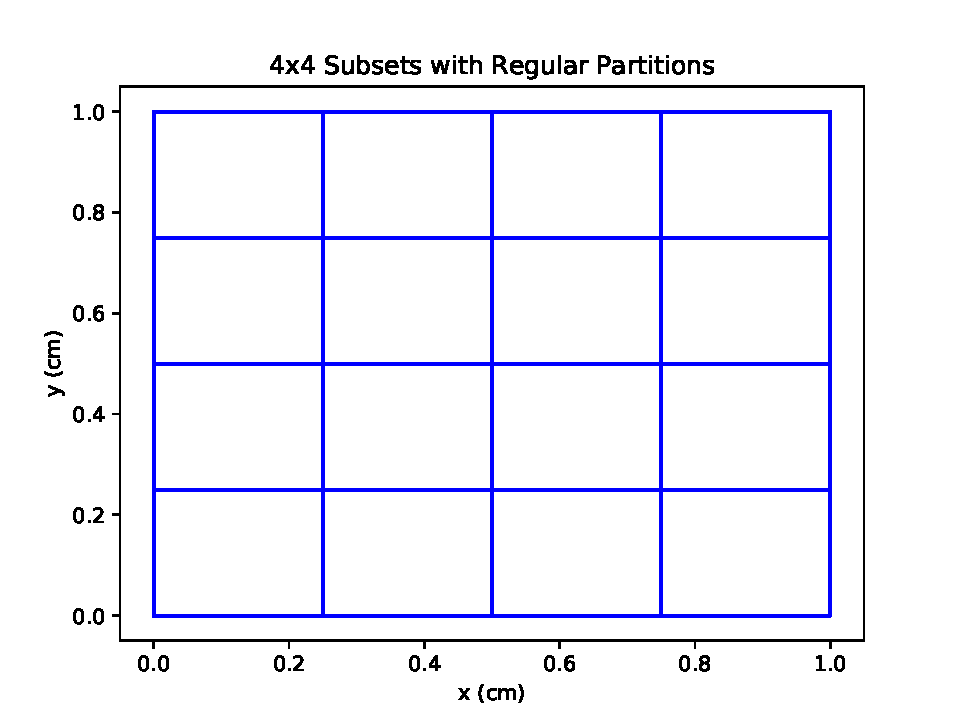
\includegraphics[width=\textwidth]{../cut_line_files/4_regular.pdf}
  \caption{4x4 subsets with regular partitions.}
  \label{4regular}
\end{subfigure}
\begin{subfigure}[b]{0.45\textwidth}
  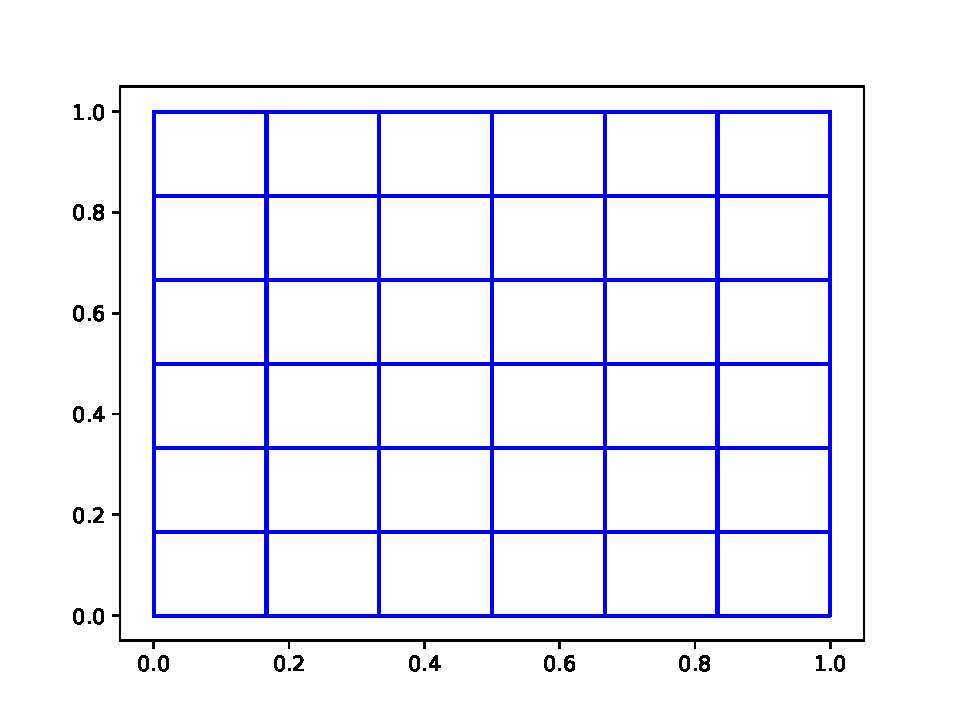
\includegraphics[width=\textwidth]{../cut_line_files/6_regular.pdf}
  \caption{6x6 subsets with regular partitions.}
  \label{6regular}
\end{subfigure}

\begin{subfigure}[b]{0.45\textwidth}
  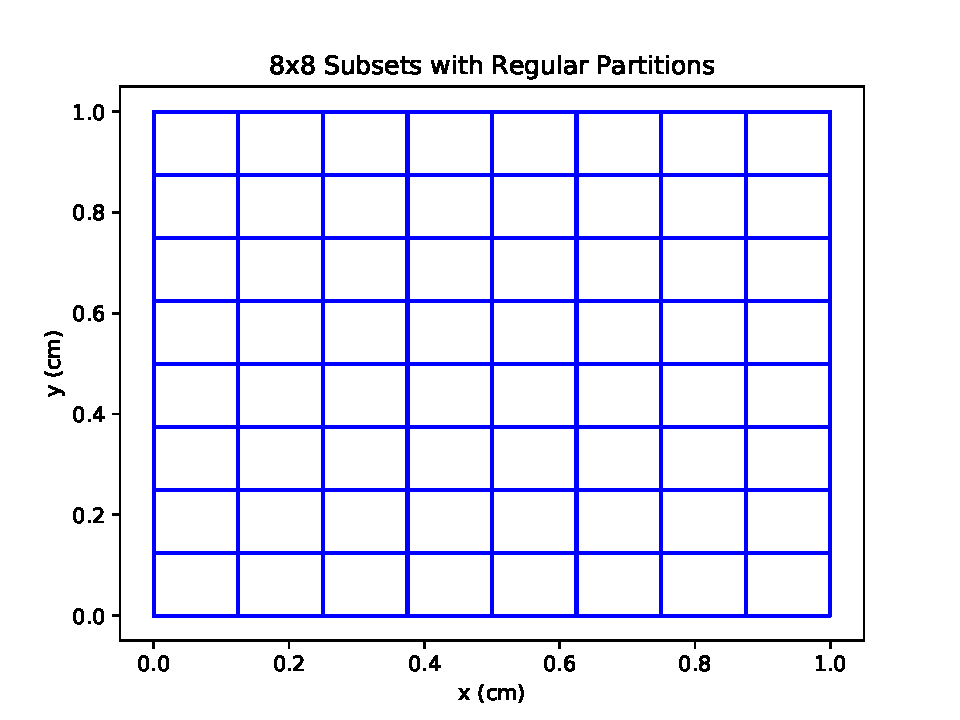
\includegraphics[width=\textwidth]{../cut_line_files/8_regular.pdf}
  \caption{8x8 subsets with regular partitions.}
  \label{8regular}
\end{subfigure}
\begin{subfigure}[b]{0.45\textwidth}
  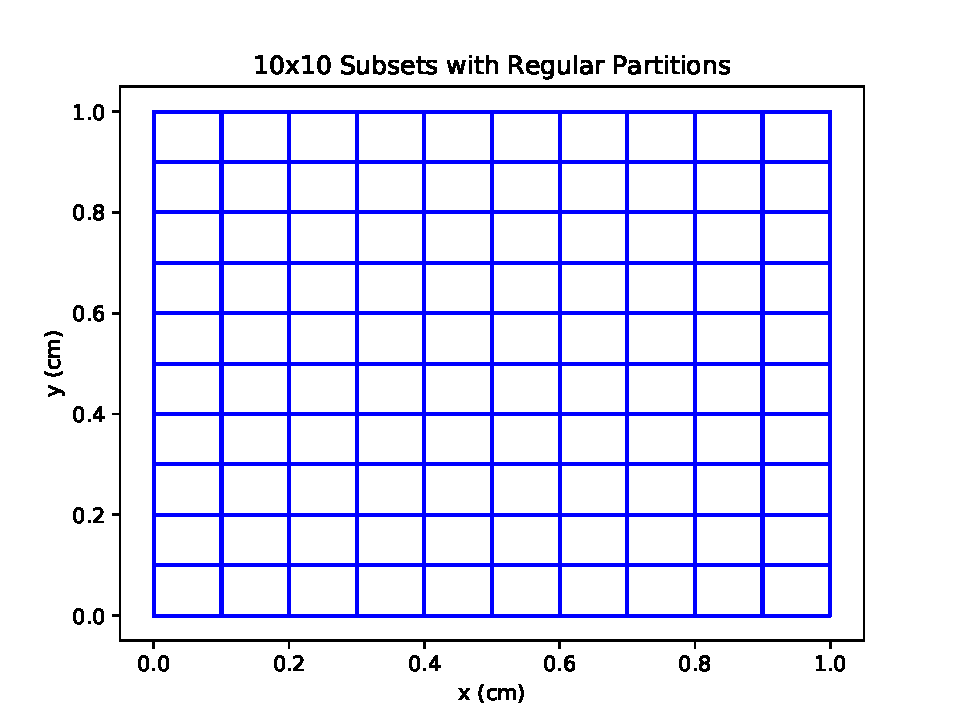
\includegraphics[width=\textwidth]{../cut_line_files/10_regular.pdf}
  \caption{10x10 subsets with regular partitions.}
  \label{10regular}
\end{subfigure}
\caption{Examples of regular partitioning.}
\label{regular_partitions}
\end{figure}

%Verification plots.
\begin{figure}[H]
\centering
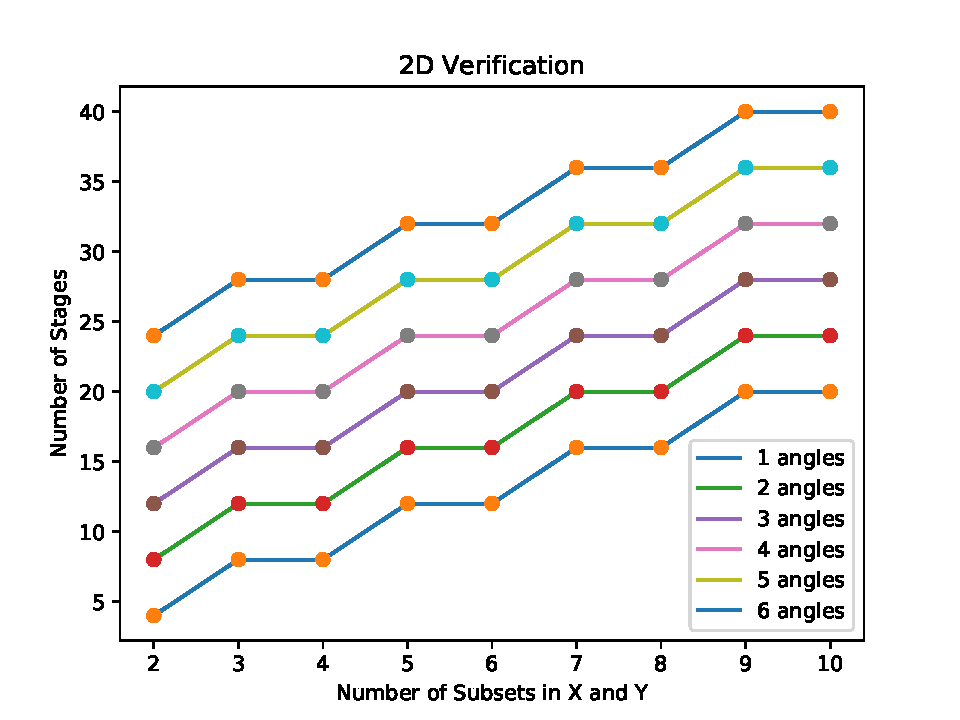
\includegraphics[scale=0.8]{../figures/regular_verification.pdf}
\caption{A 2D verification suite with regular partitions run from 2x2 to 10x10 subsets with each case being run from 1 to 6 angles per quadrant.}
\label{regular_verification}
\end{figure}

\subsection{Mildly Random Partitions}
%Mild random partitions
\begin{figure}[H]
\centering
\begin{subfigure}[b]{0.45\textwidth}
  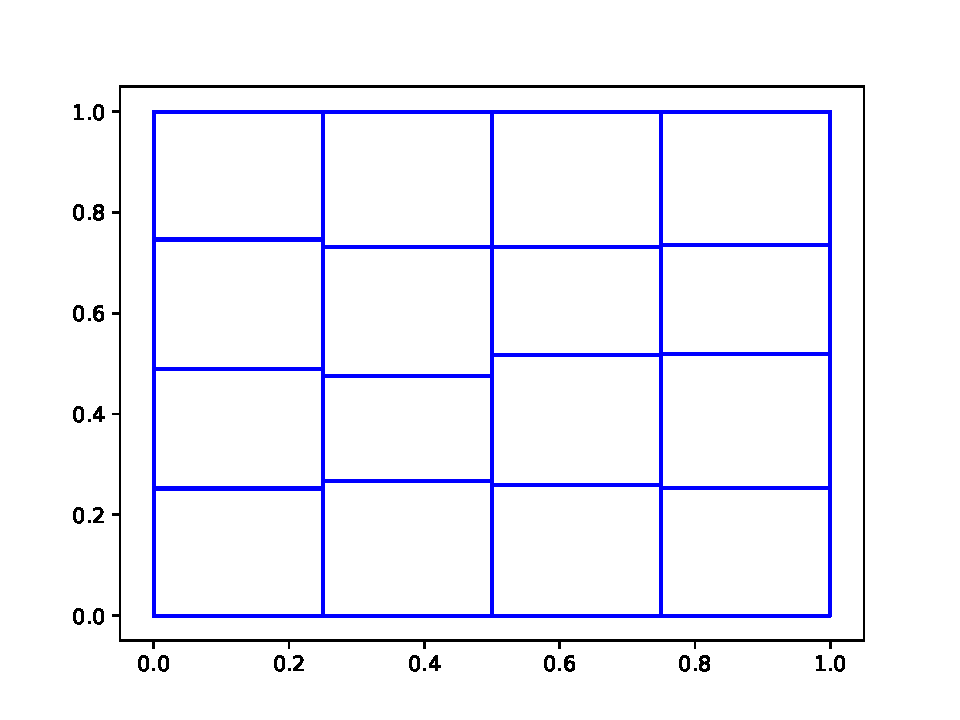
\includegraphics[width=\textwidth]{../cut_line_files/4_mild_random.pdf}
  \caption{4x4 subsets with mildly random partitions.}
  \label{4mildrandom}
\end{subfigure}
\begin{subfigure}[b]{0.45\textwidth}
  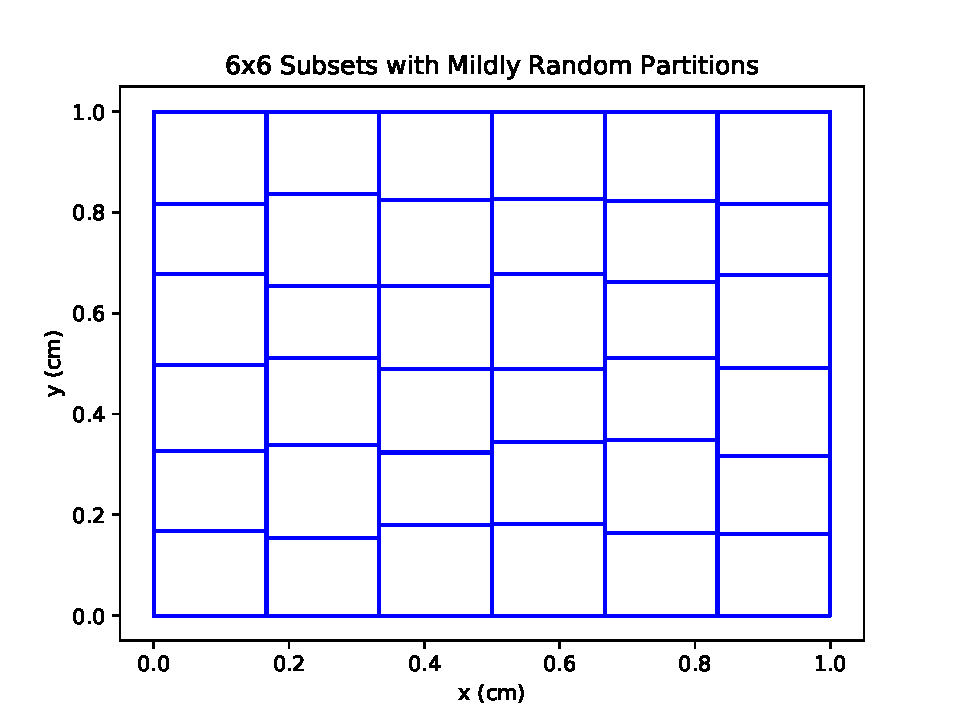
\includegraphics[width=\textwidth]{../cut_line_files/6_mild_random.pdf}
  \caption{6x6 subsets with mildly random partitions.}
  \label{6mildrandom}
\end{subfigure}

\begin{subfigure}[b]{0.45\textwidth}
  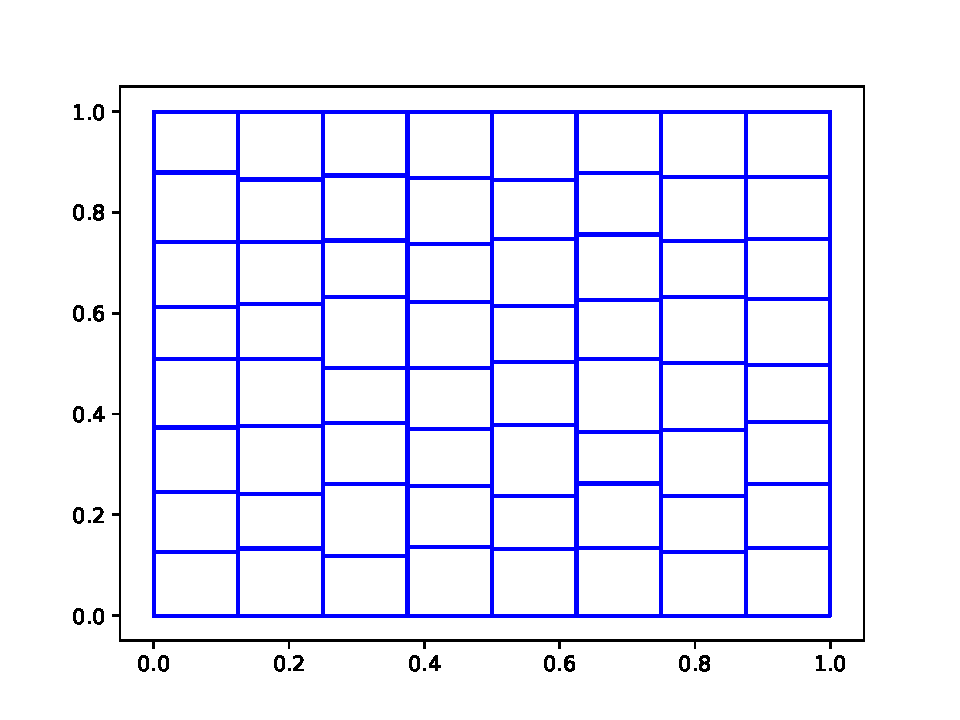
\includegraphics[width=\textwidth]{../cut_line_files/8_mild_random.pdf}
  \caption{8x8 subsets with mildly random partitions.}
  \label{8mildrandom}
\end{subfigure}
\begin{subfigure}[b]{0.45\textwidth}
  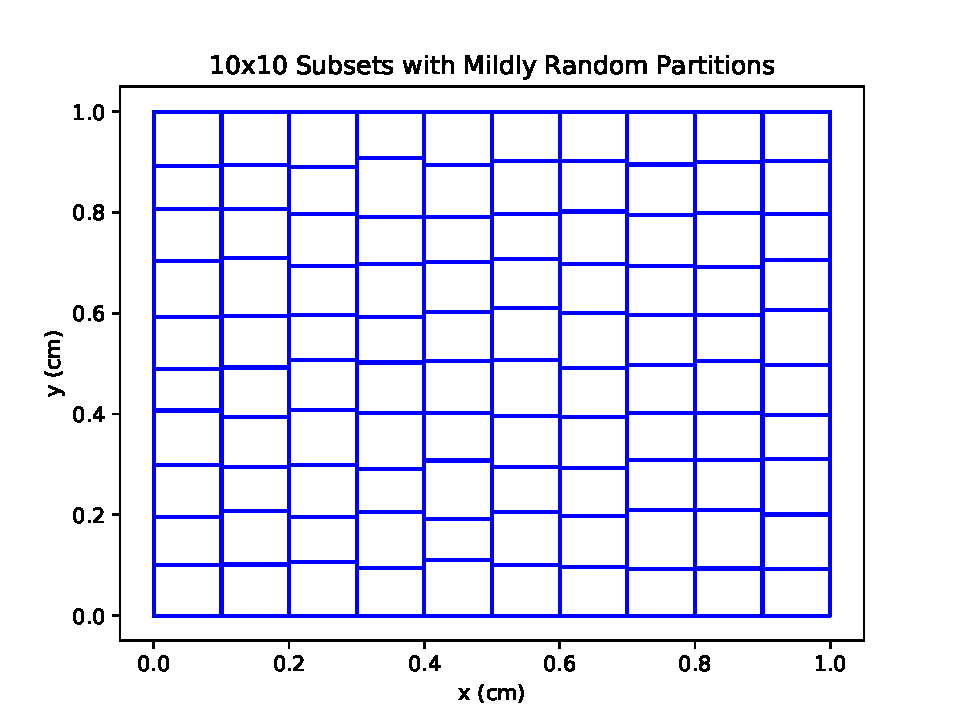
\includegraphics[width=\textwidth]{../cut_line_files/10_mild_random.pdf}
  \caption{10x10 subsets with mildly random partitions.}
  \label{10mildrandom}
\end{subfigure}
\caption{Examples of mildly random partitioning.}
\label{mild_random_partitions}
\end{figure}

\begin{figure}[H]
\centering
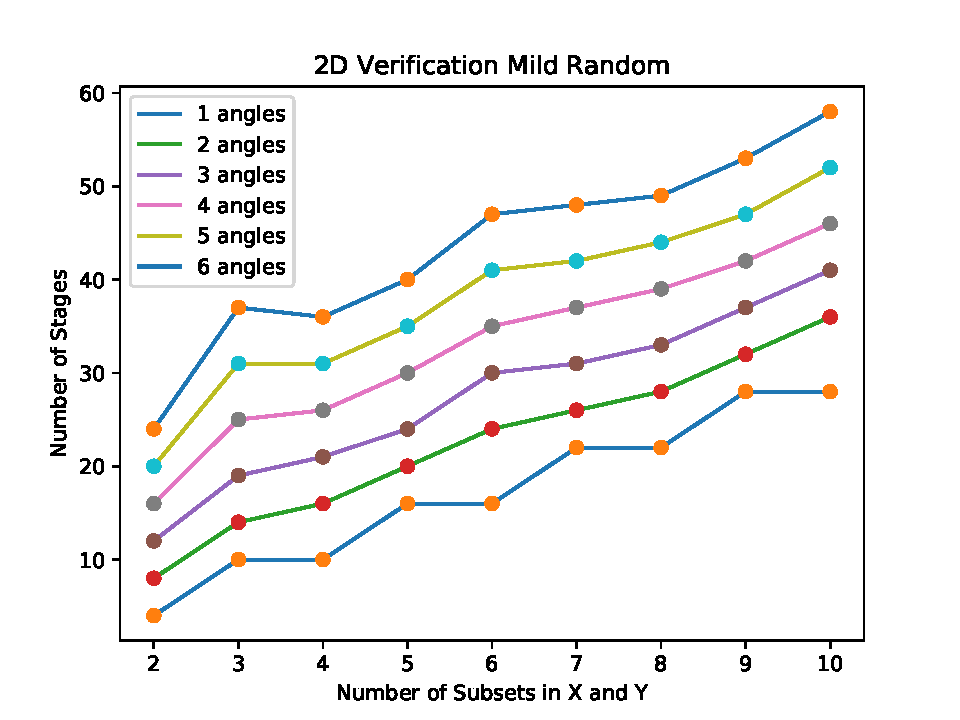
\includegraphics[scale=0.8]{../figures/mild_random_verification.pdf}
\caption{A 2D verification suite with mildly random partitions run from 2x2 to 10x10 subsets with each case being run from 1 to 6 angles per quadrant.}
\label{mild_random_verification}
\end{figure}

\subsection{Random Partitions}
%Random partitions
\begin{figure}[H]
\centering
\begin{subfigure}[b]{0.45\textwidth}
  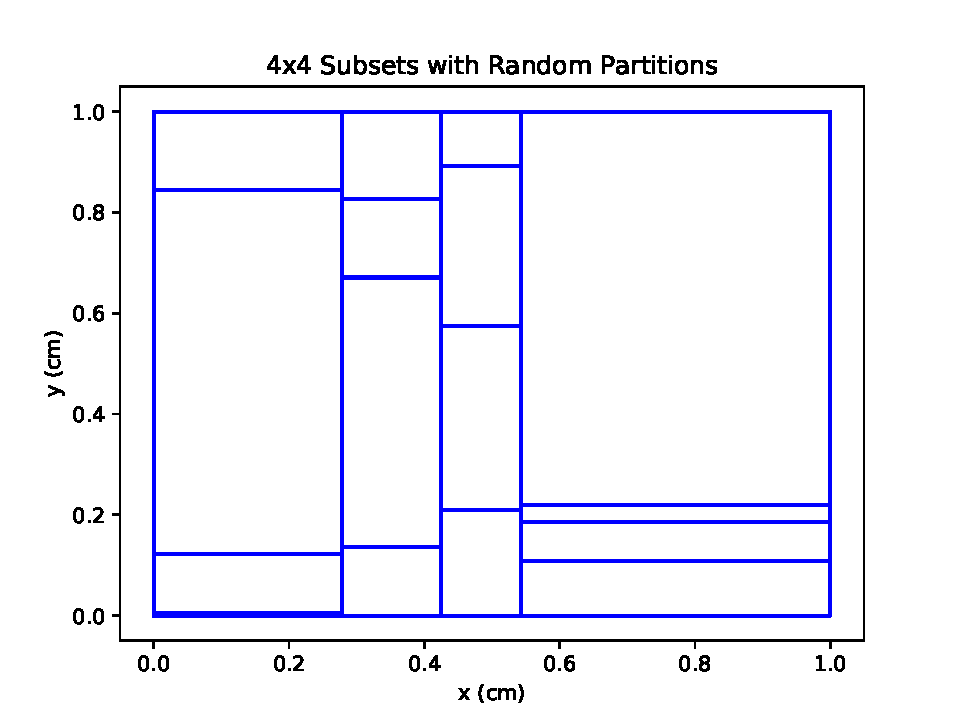
\includegraphics[width=\textwidth]{../cut_line_files/4_random.pdf}
  \caption{4x4 subsets with random partitions.}
  \label{4random}
\end{subfigure}
\begin{subfigure}[b]{0.45\textwidth}
  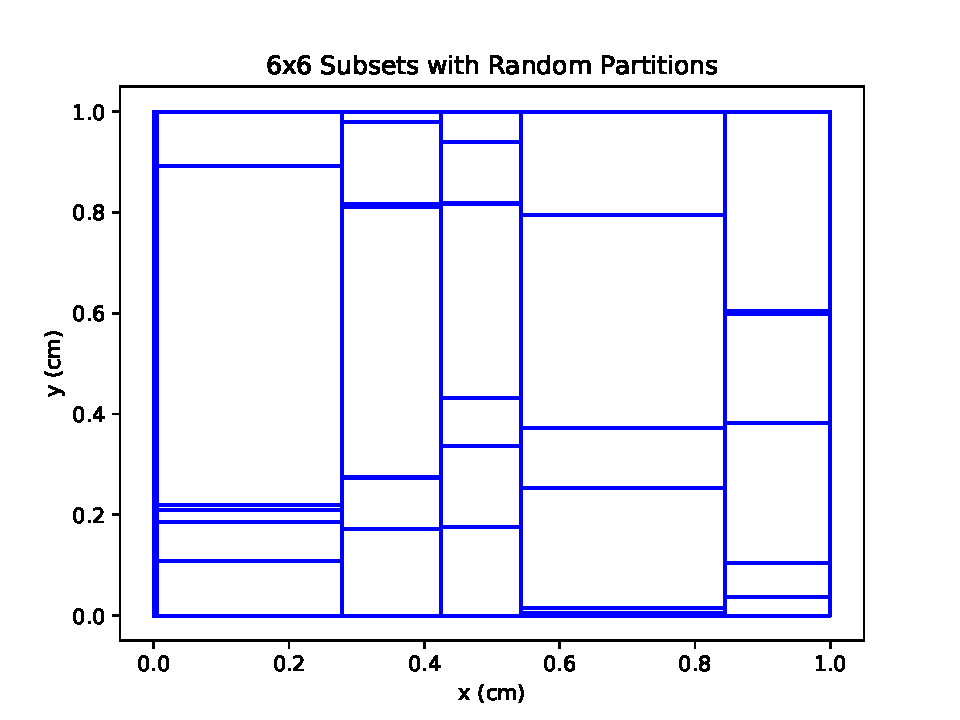
\includegraphics[width=\textwidth]{../cut_line_files/6_random.pdf}
  \caption{6x6 subsets with random partitions.}
  \label{6random}
\end{subfigure}

\begin{subfigure}[b]{0.45\textwidth}
  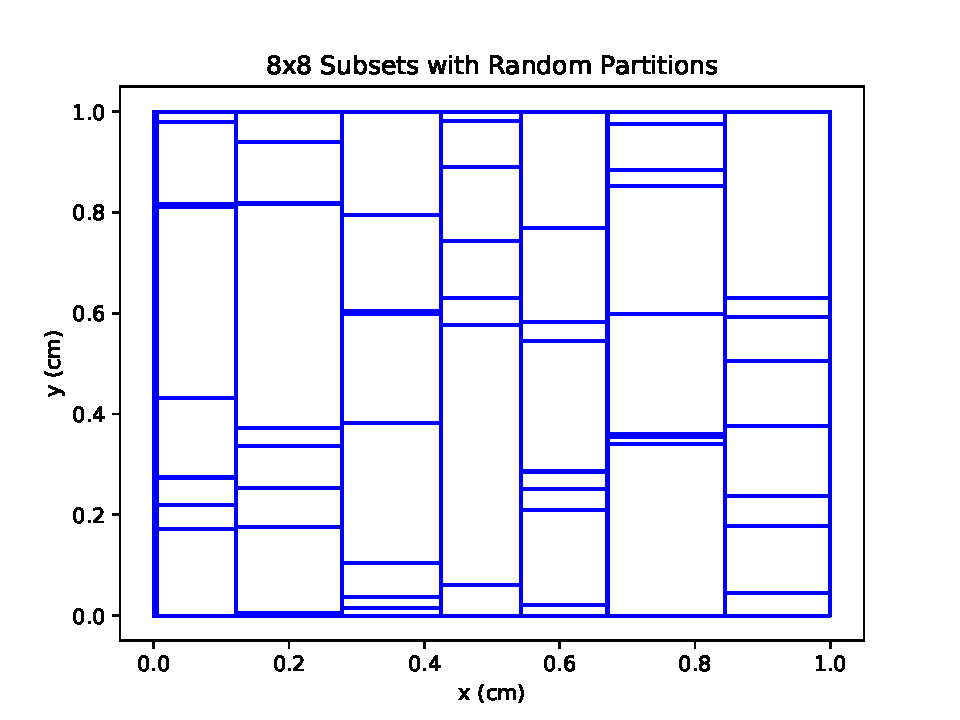
\includegraphics[width=\textwidth]{../cut_line_files/8_random.pdf}
  \caption{8x8 subsets with random partitions.}
  \label{8random}
\end{subfigure}
\begin{subfigure}[b]{0.45\textwidth}
  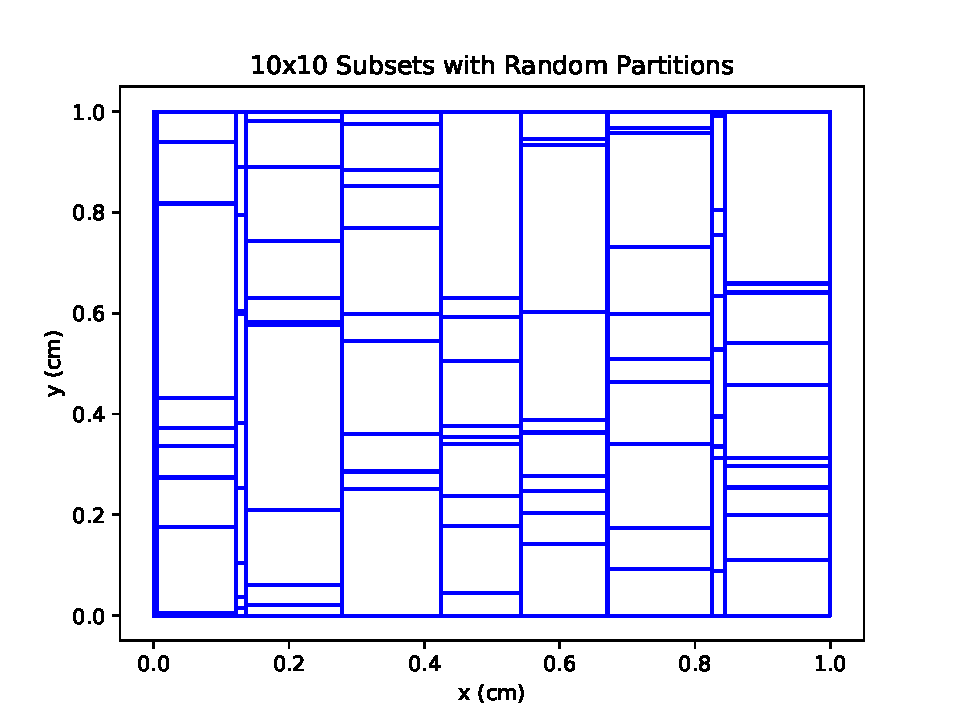
\includegraphics[width=\textwidth]{../cut_line_files/10_random.pdf}
  \caption{10x10 subsets with random partitions.}
  \label{10random}
\end{subfigure}
\caption{Examples of random partitioning.}
\label{random_partitions}
\end{figure}

\begin{figure}[H]
\centering
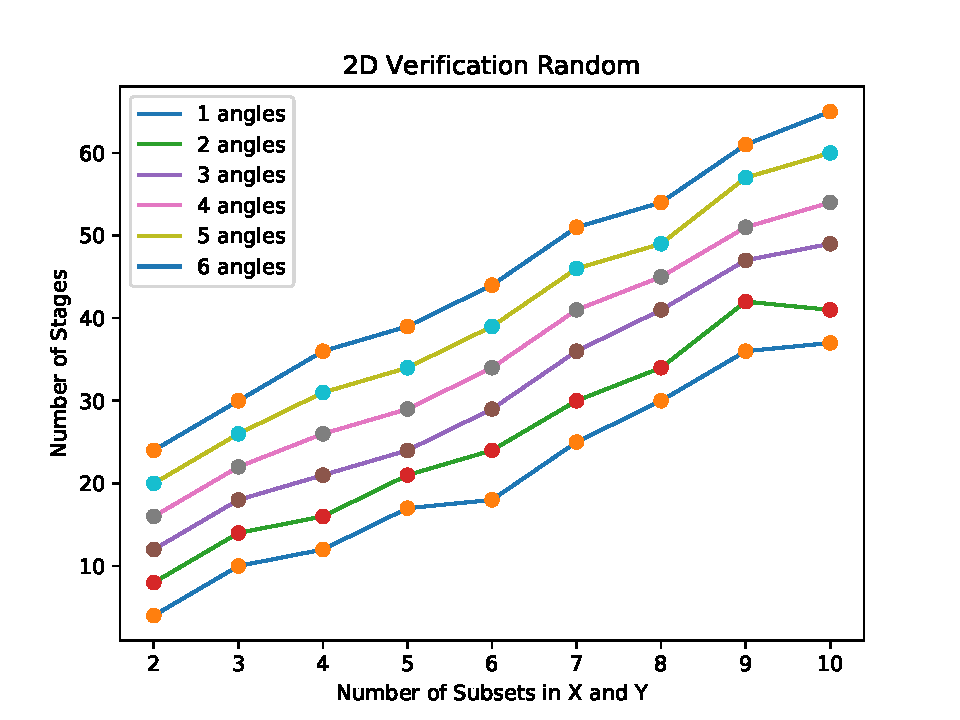
\includegraphics[scale=0.8]{../figures/random_verification.pdf}
\caption{A 2D verification suite with random partitions run from 2x2 to 10x10 subsets with each case being run from 1 to 6 angles per quadrant.}
\label{random_verification}
\end{figure}

\subsection{Probable Worst-Case Partitions}
\begin{figure}[H]
\centering
\begin{subfigure}[b]{0.45\textwidth}
  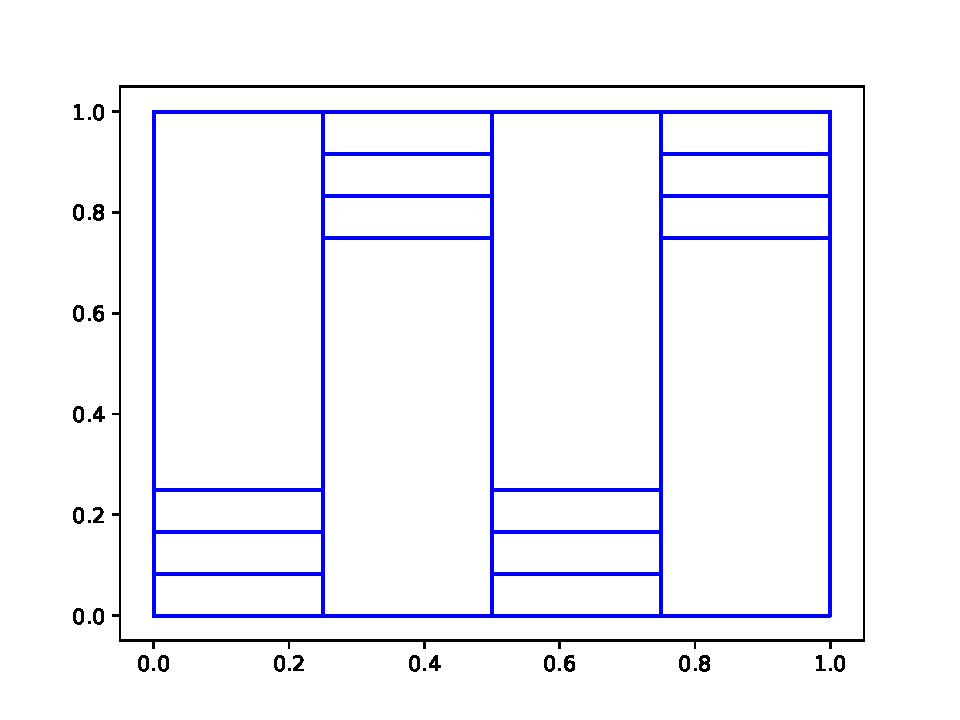
\includegraphics[width=\textwidth]{../cut_line_files/4_worst.pdf}
  \caption{4x4 subsets with probable worst-case partitions.}
  \label{4worst}
\end{subfigure}
\begin{subfigure}[b]{0.45\textwidth}
  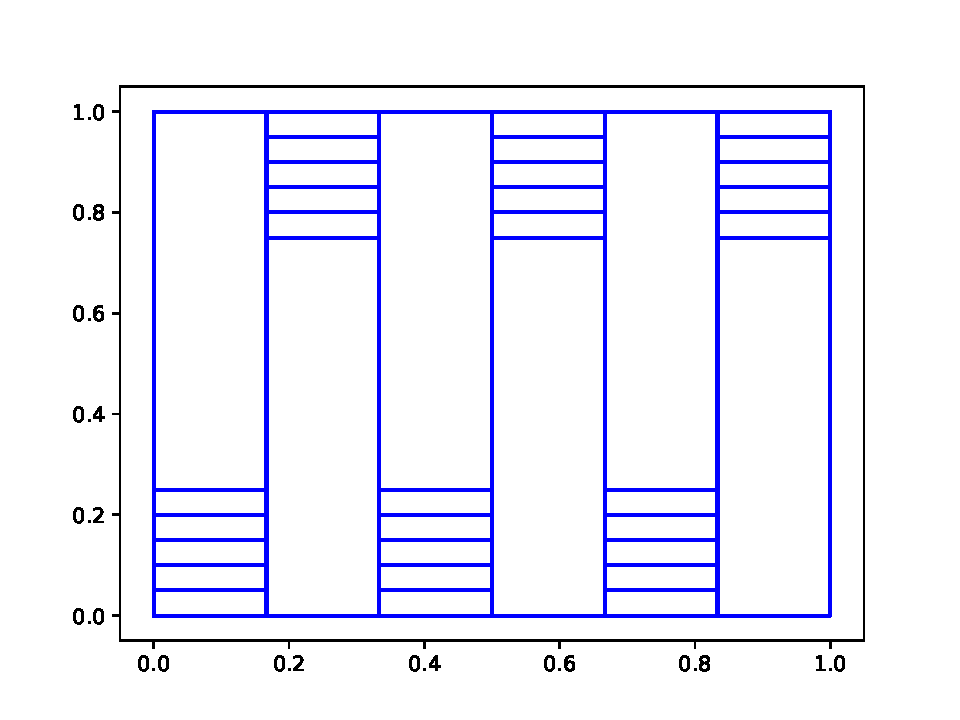
\includegraphics[width=\textwidth]{../cut_line_files/6_worst.pdf}
  \caption{6x6 subsets with probable worst-case partitions.}
  \label{6worst}
\end{subfigure}

\begin{subfigure}[b]{0.45\textwidth}
  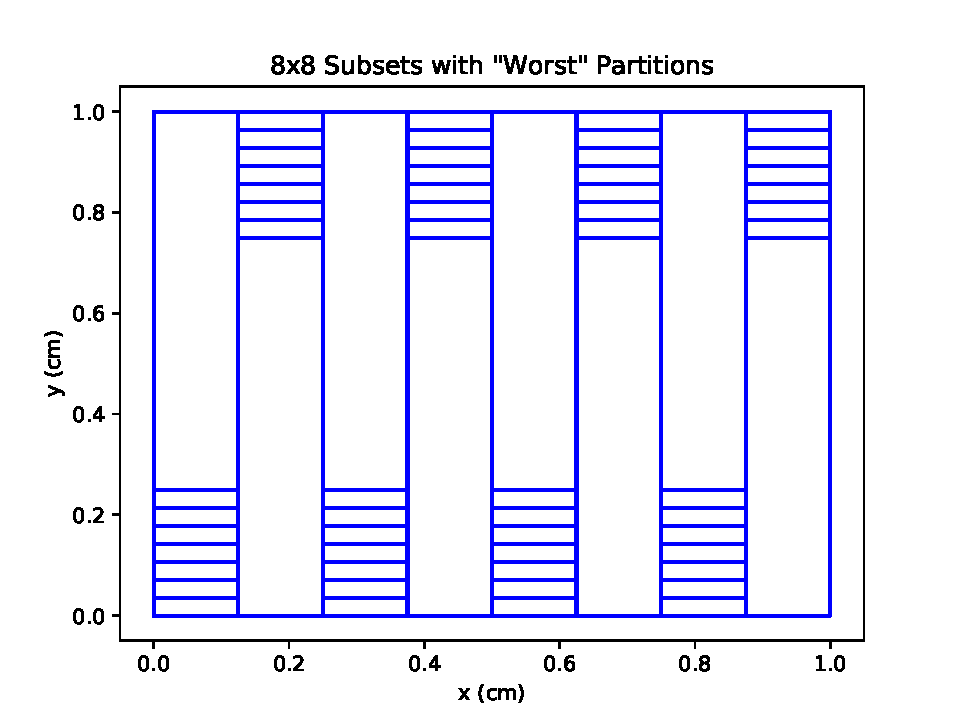
\includegraphics[width=\textwidth]{../cut_line_files/8_worst.pdf}
  \caption{8x8 subsets with probable worst-case partitions.}
  \label{8random}
\end{subfigure}
\begin{subfigure}[b]{0.45\textwidth}
  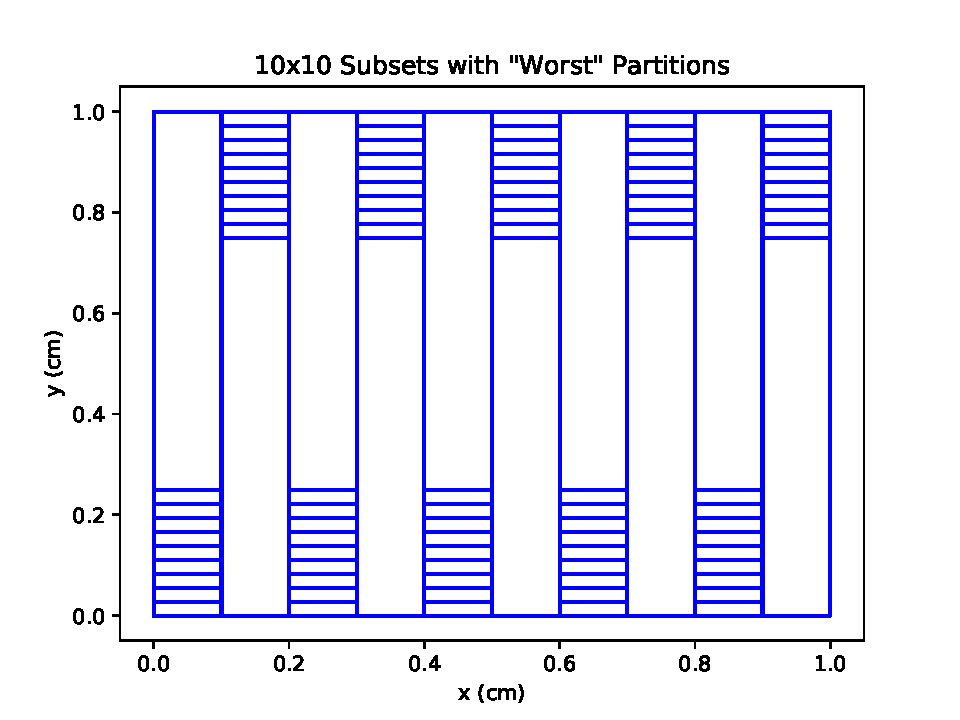
\includegraphics[width=\textwidth]{../cut_line_files/10_worst.pdf}
  \caption{10x10 subsets with probable worst-case partitions.}
  \label{10random}
\end{subfigure}
\caption{Examples of probable worst-case partitioning.}
\label{worst_partitions}
\end{figure}

\begin{figure}[H]
\centering
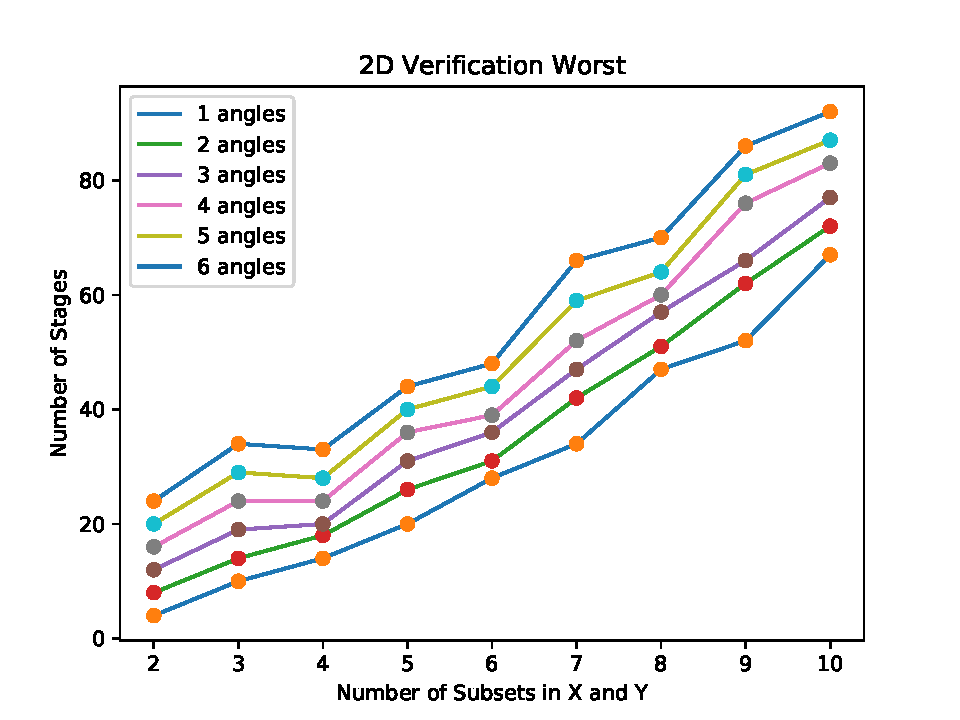
\includegraphics[scale=0.8]{../figures/worst_verification.pdf}
\caption{A 2D verification suite with probable worst-case partitions run from 2x2 to 10x10 subsets with each case being run from 1 to 6 angles per quadrant.}
\label{worst_verification}
\end{figure}

\section{3D Verification}

The 3d verification results will go here.

%%%%%%%%%%%%%%%%%%%%%%%%%%%%%%%%%%%%%%%%%%%%%%%%%%%
%
%  New template code for TAMU Theses and Dissertations starting Fall 2016.
%
%
%  Author: Sean Zachary Roberson
%  Version 3.17.09
%  Last Updated: 9/21/2017
%
%%%%%%%%%%%%%%%%%%%%%%%%%%%%%%%%%%%%%%%%%%%%%%%%%%%
%%%%%%%%%%%%%%%%%%%%%%%%%%%%%%%%%%%%%%%%%%%%%%%%%%%%%%%%%%%%%%%%%%%%%%
%%                           TIME TO SOLUTION ESTIMATOR CHAPTER
%%%%%%%%%%%%%%%%%%%%%%%%%%%%%%%%%%%%%%%%%%%%%%%%%%%%%%%%%%%%%%%%%%%%%



\chapter{PARTITIONING OPTMIZIATION \label{cha:optimization}}
\jcr{definitely needs an introduction to the chapter. by the way, make sure all chapters have a decent introduction ...}\\
jcr{I will not read too much the text here. I feel this is a rough draft. I'll look at the results instead.}

\section{Method}
With confidence in the time-to-solution estimator, it is used as the objective function in two optimization methods. The first optimization method utilizes scipy's optimize library, and the second method utilizes knowledge of a problem's mesh layout to assist in partition placement.
%%%%%%%%%%%%%%%%%%%%%%%%%%%%
\subsection{Scipy optimize}
  The scipy optimize library \cite{scipy} provides many tools for optimizing an input function with local and global minimization techniques. Our usage of the optimize library relies on the minimize function, using the basinhopping \cite{basinhoppingwales} method as the global optimizer, and the constrained Nelder-Mead method as the local optimizer.

\subsection{``Human'' Optimization}
\jcr{here, I want to use the term CDF used. By the way, you need to make sure the mesh CDF's are defined way earlier, in a previous chapter, as appropriate...}

  The ``black box'' method using scipy optimize's basinhopping and constrained Nelder-Mead minimizers is functional for small parameter spaces. However, even with modestly large parameter spaces such as the one seen in the Level 2 experiment (Fig. \ref{level2_nocut}), the time-to-solution estimator function is not smooth enough for scipy optimize to honor the constraints or bounds of the problem, leading to the time-to-solution estimator crashing. This lead to the development of an alternative method.

  The ``human optimization'' method utilizes the geometrical information of the problem to attempt to find optimal cuts. This method prioritizes finding cut line locations that cut along a ``natural boundary''. A natural boundary is a subset boundary that coincides with the geometrical features of the mesh. In Fig. \ref{natural_boundary_example}, we notice natural boundaries every centimeter in each dimension.
 \begin{figure}[h]
\centering
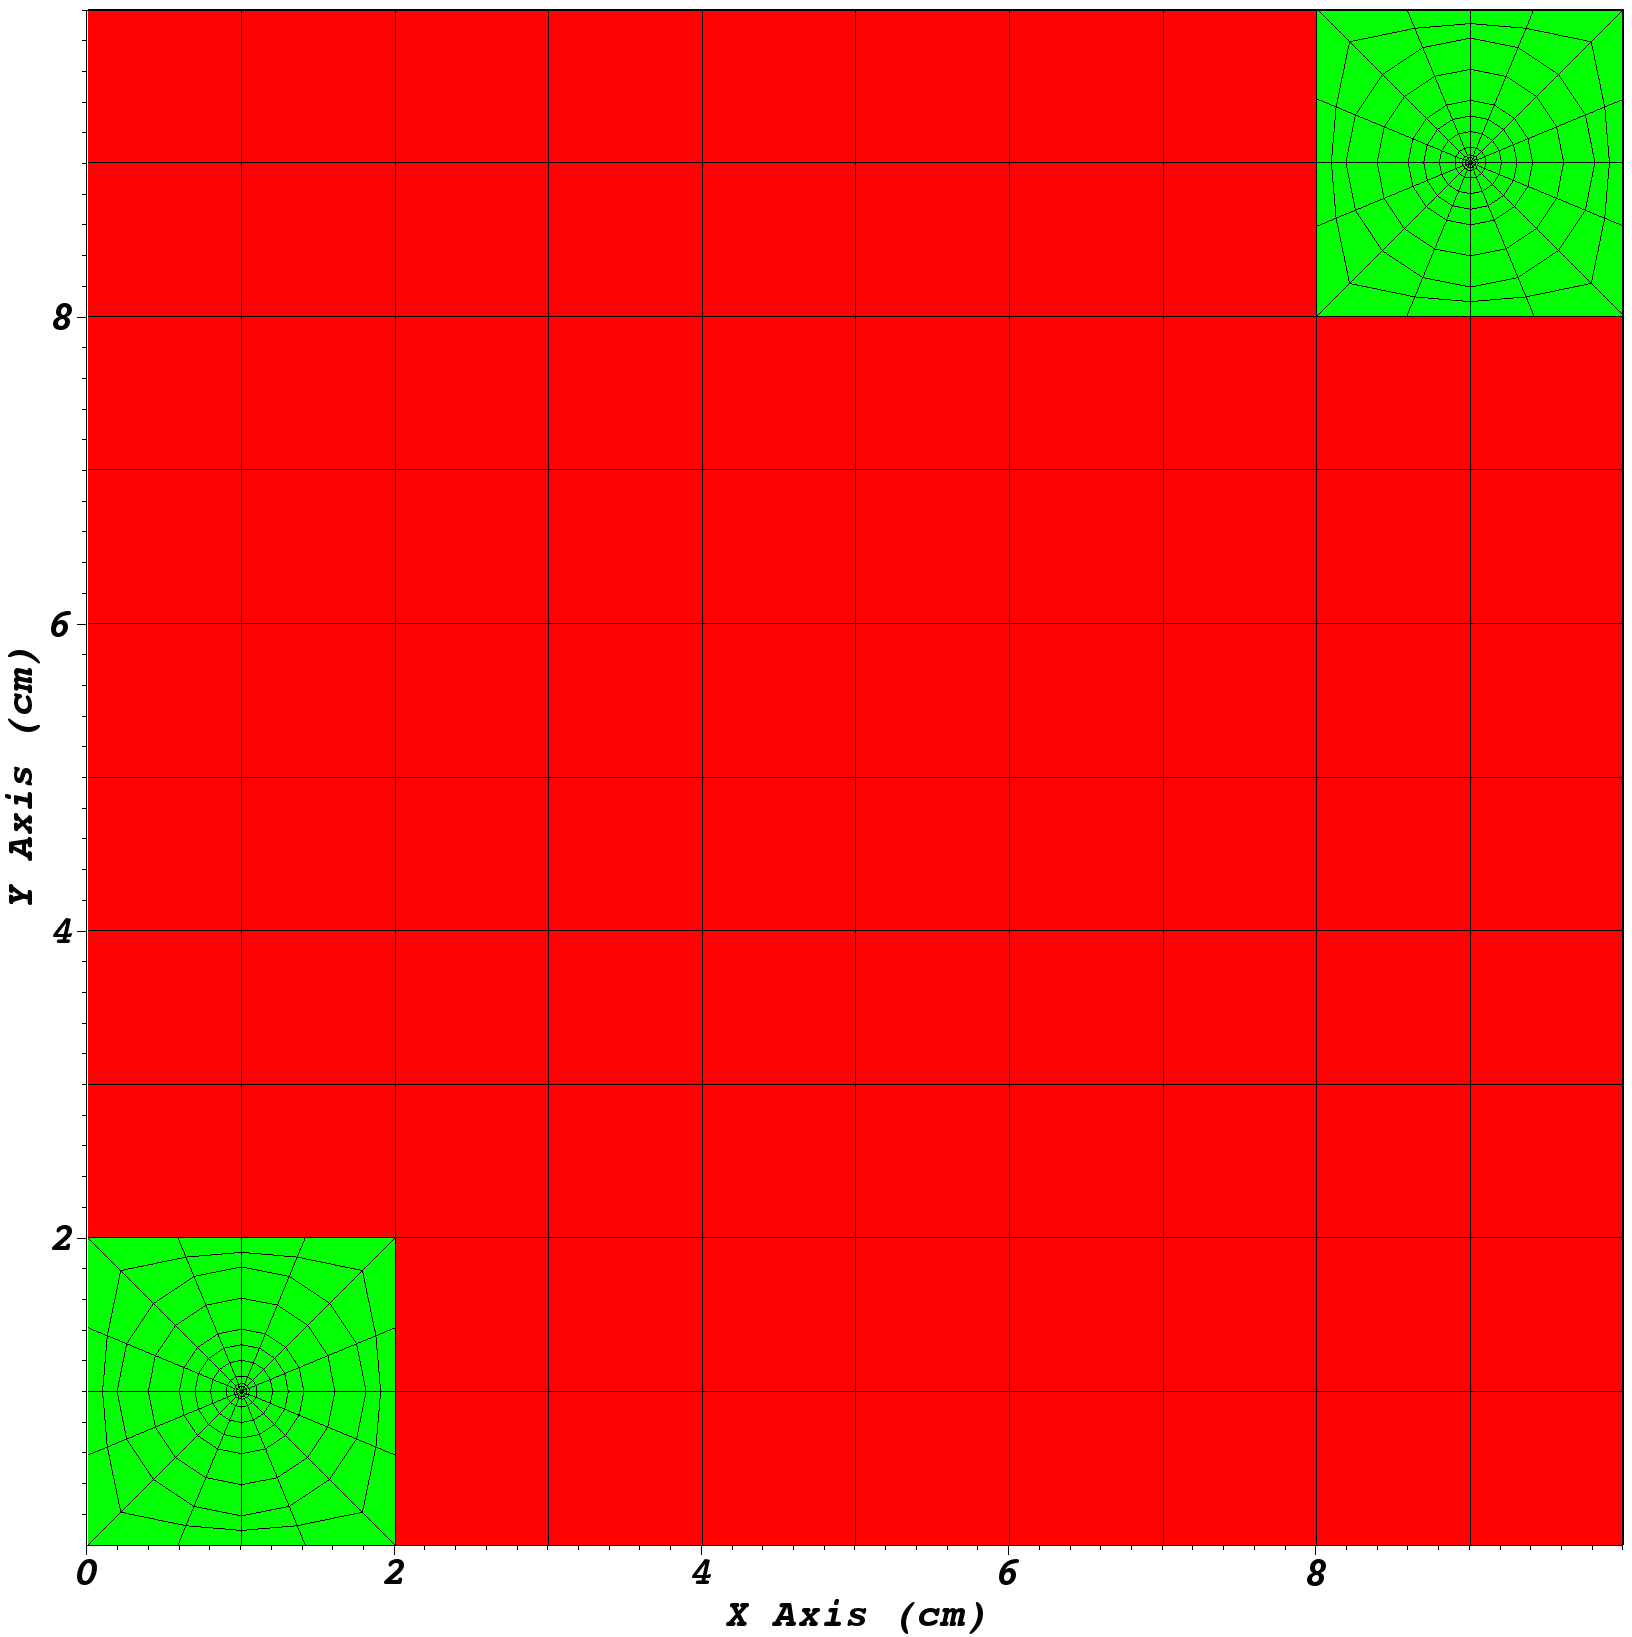
\includegraphics[scale=0.2]{../figures/spiderweb_10x10_sparse.png}
\caption{An unstructured mesh with natural boundaries at 1 cm intervals in both dimensions.}
\label{natural_boundary_example}
\end{figure}

This optimization method:
\begin{enumerate}
  \item Find the most suitable natural boundaries in the $x$ dimension.
  \item For each set of columns, find the most suitable natural boundaries in the $y$ dimension.
  \item Run all iterations of cut lines selected.
\end{enumerate}

\subsubsection{Finding natural boundaries}

In order to identify natural boundaries, we analyze the detailed cumulative distribution function (CDF) of the vertices in each dimension. The jumps in the CDF correspond to natural boundaries. Figure \ref{vert_cdf} shows the x-vertex CDF of the mesh in Fig. \ref{natural_boundary_example}.
\begin{figure}[h]
\centering
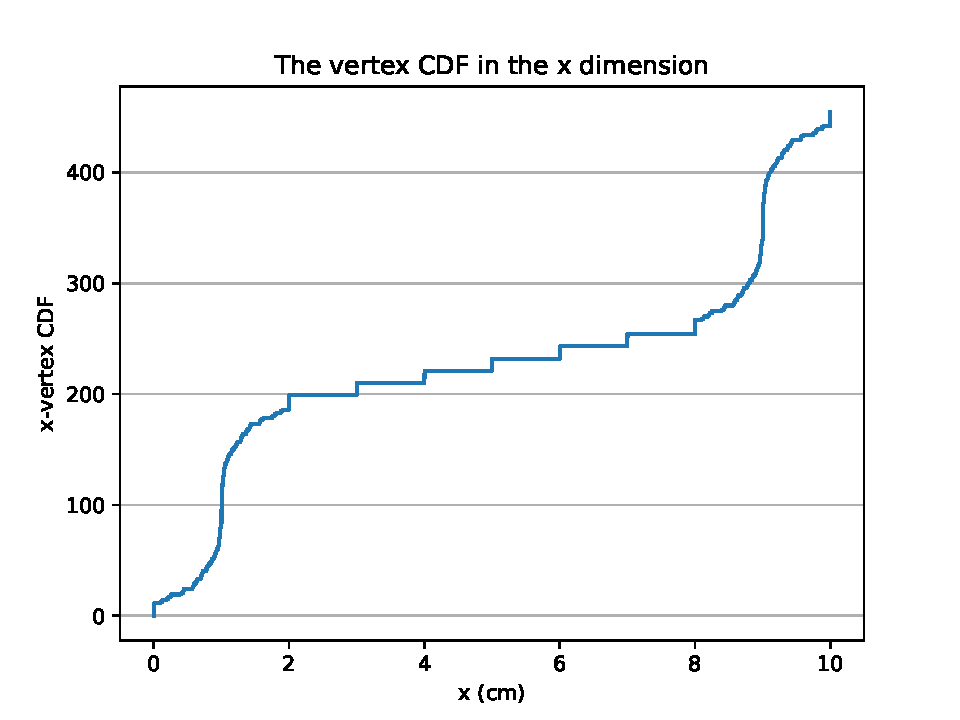
\includegraphics[scale=0.75]{../figures/xvertexcdf.pdf}
\caption{The x-vertex CDF of the mesh shown in Fig. \ref{natural_boundary_example}}.
\label{vert_cdf}
\end{figure}

To identify where the jumps in the CDF occur, we take the gradient\jcr{I think your CDF's are functions of 1 variable only, so it's a derivative, no?} of the CDF and isolate the largest discontinuities in it. Figure \ref{gradcdf} plots the gradient of the CDF shown in Fig. \ref{vert_cdf}. \jcr{not sure I understand the jumps in the CDF derivative at the beginning and the end of the x axis. Why is it jumping? Numerical artifact? }
\begin{figure}[h]
\centering
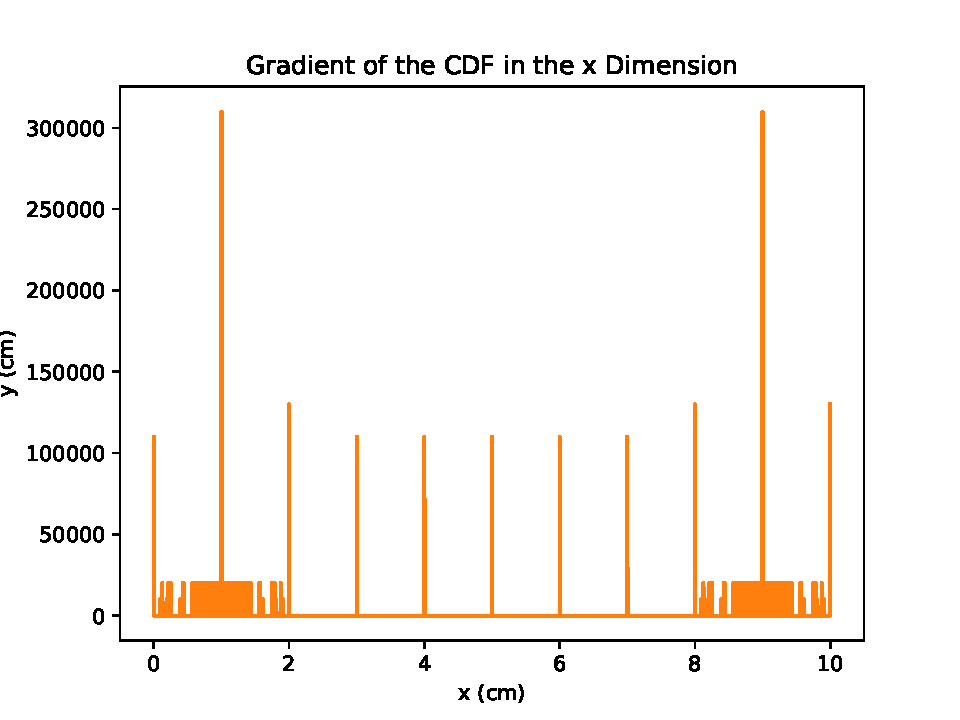
\includegraphics[scale=0.75]{../figures/gradcdf.pdf}
\caption{The gradient of the CDF shown in Fig. \ref{vert_cdf}}.
\label{gradcdf}
\end{figure}
The largest discontinuities in Fig. \ref{gradcdf} occur at the instances where there are natural boundaries all the way through the mesh, or at 1 cm intervals.

\FloatBarrier
\subsubsection{Finding natural boundaries for sets of columns}
In order to globalize the optimization of the cut lines per column, we set up a binary tree of test cases, such as the one shown in Fig. \ref{binary_tree}. Each layer in the tree represents one set of $y$ cut lines. The first layer, or the root of the tree, represents the case where we try and find the natural boundaries in $y$ throughout all columns, in this case 4 columns. The next layer tries to find two sets of natural boundaries, one set of natural $y$ boundaries through the first two columns, and another set through the final 2 columns. Finally, the last case finds a set of natural $y$ boundaries in each individual column.

\begin{figure}[h]
\centering
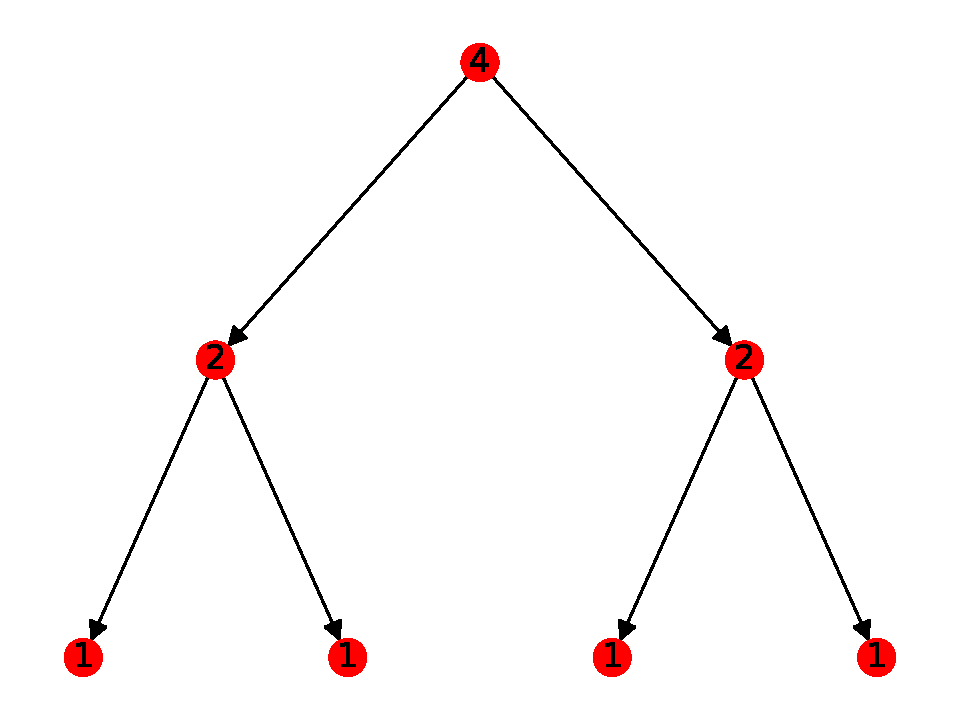
\includegraphics[scale=0.75]{../figures/binary_tree.pdf}
\caption{A binary tree where each node represents the number of columns we are attempting to find a natural boundary through.}
\label{binary_tree}
\end{figure}

Let's consider the mesh of the Level 2 experiment shown in Fig. \ref{level2_nocut}.

\begin{figure}[h]
\centering
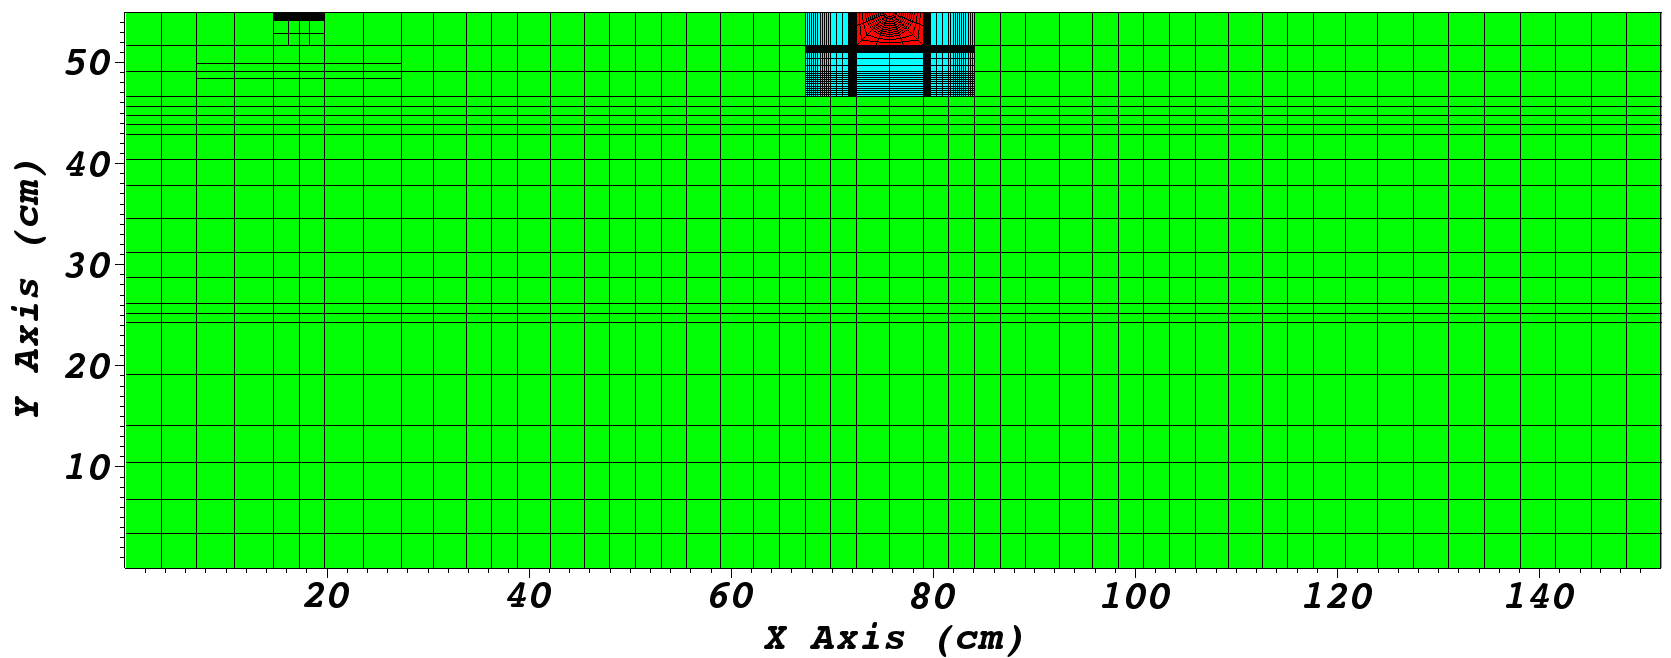
\includegraphics[scale=0.3]{../../figures/level2_nocut.png}
\caption{The mesh for the Level 2 experiment.}
\label{level2_nocut}
\end{figure}

\begin{figure}[h]
\centering
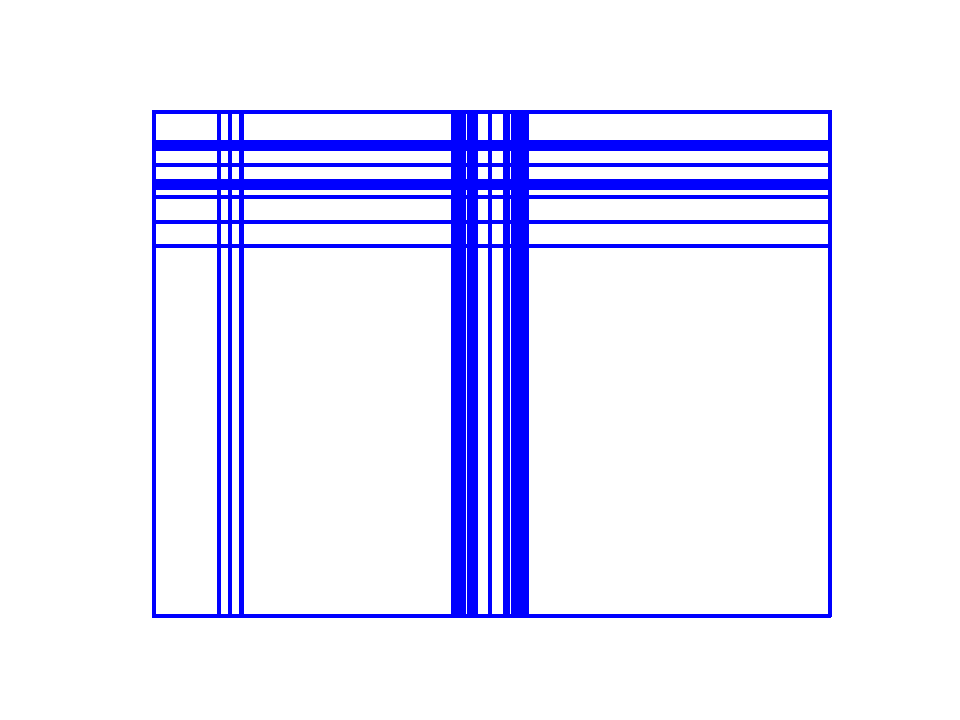
\includegraphics[scale=0.55]{../../figures/lvl2_suite_0.pdf}
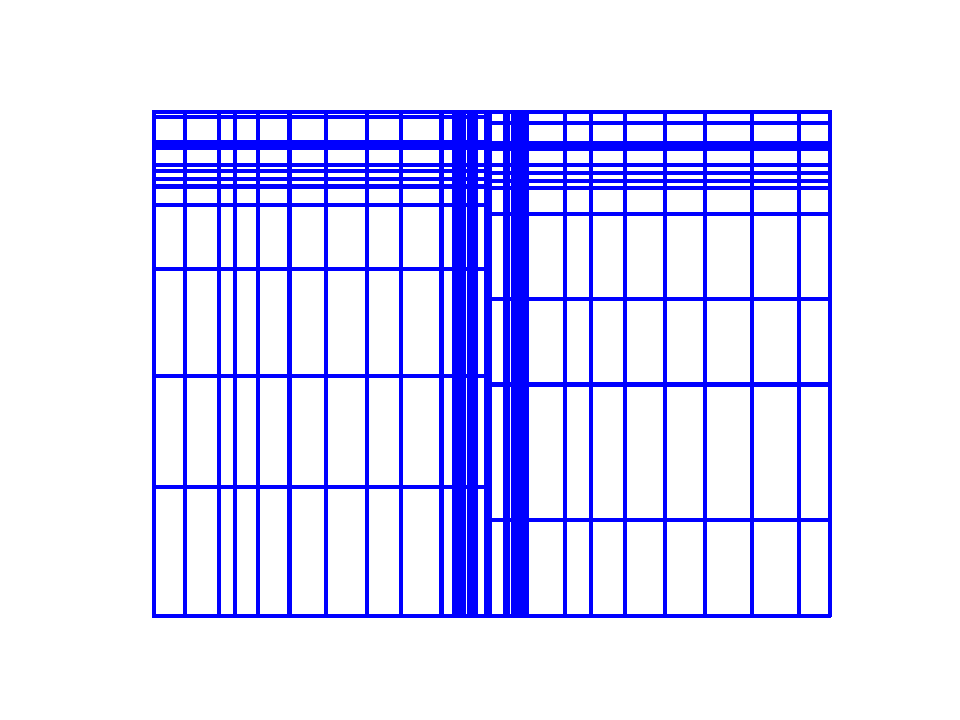
\includegraphics[scale=0.55]{../../figures/lvl2_suite_1.pdf}
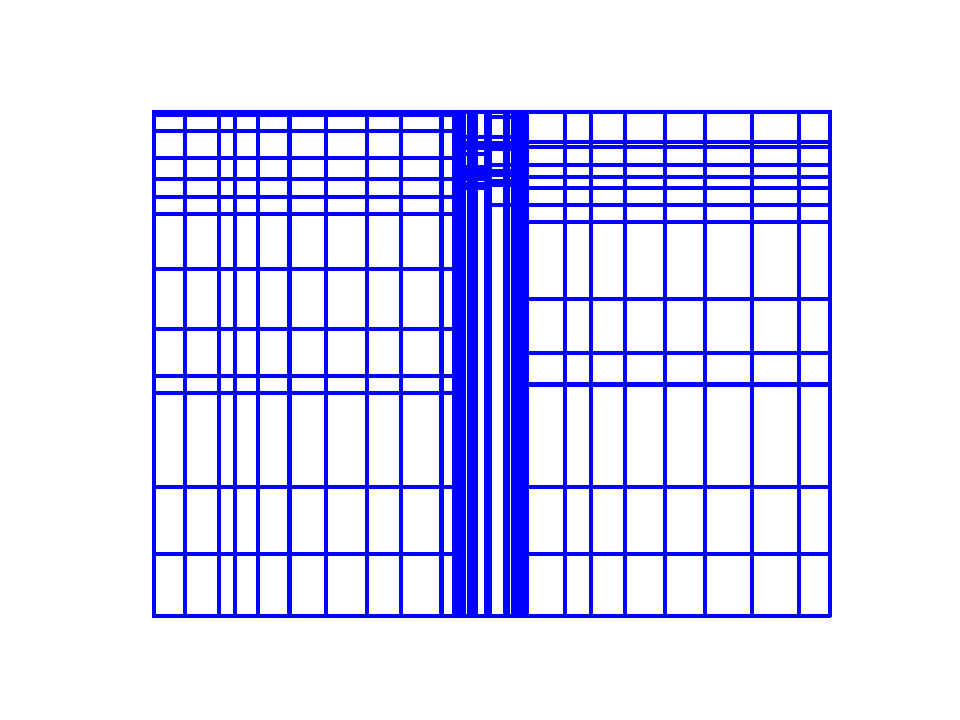
\includegraphics[scale=0.55]{../../figures/lvl2_suite_2.pdf}
\end{figure}

\FloatBarrier

\section{PDT Comparison Results}

The PDT comparison goes here.

%%%%%%%%%%%%%%%%%%%%%%%%%%%%%%%%%%%%%%%%%%%%%%%%%%%
%
%  New template code for TAMU Theses and Dissertations starting Fall 2016.
%
%
%  Author: Sean Zachary Roberson
%  Version 3.17.09
%  Last Updated: 9/21/2017
%
%%%%%%%%%%%%%%%%%%%%%%%%%%%%%%%%%%%%%%%%%%%%%%%%%%%
%%%%%%%%%%%%%%%%%%%%%%%%%%%%%%%%%%%%%%%%%%%%%%%%%%%%%%%%%%%%%%%%%%%%%%
%%                           SECTION IV
%%%%%%%%%%%%%%%%%%%%%%%%%%%%%%%%%%%%%%%%%%%%%%%%%%%%%%%%%%%%%%%%%%%%%



\chapter{SUMMARY AND CONCLUSIONS \label{cha:Summary}}

Transport sweep techniques obtain solutions to the Boltzmann transport equation efficiently by employing discretization techniques that allow for solving the transport equation one cell at a time.
Parallelizing the transport sweep offers the ability to solve memory-intensive problems, and with parallel sweep algorithms such as KBA and PDT's hybrid KBA, this can be done efficiently.

However, when unstructured meshes are used, these algorithms can lose effectiveness as unstructured meshes can introduce imbalanced partitions.
We combat these imbalanced partitions by load balancing the meshes before sweeping them, attempting to obtain an equivalent amount of work per processor.
In Chapter \ref{cha:lb}, we saw that our two load-balancing algorithms, the original load-balancing algorithm and the load-balancing-by-dimension algorithm, can obtain close to a 90\% improvement in the cell count in the heaviest subset for unstructured meshes.
However, we noticed that a balanced problem  does not signify that it will be swept faster, somewhat defeating the purpose of achieving load balance.

Chapter \ref{cha:tts} details the time-to-solution estimator, a tool that predicts the sweep time for a given set of partitioning parameters.
PDT has had a performance model that predicted the sweep time for structured, balanced meshes, but had no way to predict the sweep time for imbalanced and staggered (where cut lines don't go all the way through the mesh) partitions.
The time-to-solution estimator has no restriction on mesh type, and can be used to predict the sweep time for balanced or imbalanced (importantly, staggered) partitions.
The estimator was run through a benchmark suite that mirrored the PDT scaling suite from 1 to 16,384 cores.
The time-to-solution estimator was within 4\% of PDT's performance model estimator for the sweep time for all problems in the scaling suite, and within 12\% of PDT's sweep time for all cases in the scaling suite (shown in Table \ref{scaling_percent_diff}).
The time-to-solution estimator was also tested against unstructured meshes, with the majority of problems run within 10\% of PDT's sweep time.

Chapter \ref{cha:optimization} describes our method for optimizing partitions.
It quickly became apparent that black box tools were not suitable for our problem, due to the time-to-solution estimator not being a smooth enough function.
A secondary method, the CDF optimization method, relies on intuitively interpreting the geometric information in an attempt to find optimal cuts.
The detailed vertex CDF is analyzed in each dimension, and jumps in the CDF correspond to locations where natural boundaries (where partition boundaries are the same as mesh boundaries) occur.
The CDF optimization method will initially select cuts that balance the mesh, then ``snap'' those cuts to natural boundaries.
This method proved effective at finding optimal partitions for the majority of cases run.

\section{Future Work}

The time-to-solution estimator allowed us to study the sweep time as a function of partitioning parameters.
Although we saw good agreement with PDT, particularly for problems with larger numbers of unknowns, we saw some discrepancies.
We hypothesize that this is due to the following three reasons:
\begin{enumerate}
\item PDT's first-come-first-serve schedule is not consistent with the time-to-solution estimator's schedule,
\item The latency on Quartz is easy to mischaracterize,
\item The machine parameters that are fed to the time-to-solution estimator are generated using structured meshes.
\end{enumerate}

The first reason, the discrepancy between the two schedules, can be remedied by feeding the time-to-solution estimator's schedule directly into PDT and having PDT use it.
I believe this would be a worthwhile project for a master's thesis in the future in order to study the effect on the results between PDT and the time-to-solution estimator.

The second reason, the mischaracterization of Quartz's latency, has three potential paths forward.
The first is to obtain allocation on a Blue-Gene/Q machine and rerun all problems in this dissertation.
Blue-Gene/Q machines tend to have more stable latencies than x86 machines (such as Quartz), and as such can be more easily characterized.
Results obtained on a Blue-Gene/Q machine would confirm the x86 noise as a source of discrepancy.
The second path forward to this problem is to attempt to generate latency information for different core counts for x86 machines, rather than have a flat multiplier regardless of core count.
The last path forward is to recognize that there is an inherent randomness in the latency on x86 machines, and account for that in the latency term in the time-to-solution estimator.

The third and final reason, the generation of machine parameters, also lends itself to subsequent investigations.
Generating the empirical constants used in the time-to-solution estimator should be done with both structured and unstructured meshes to check if the constants' values change significantly.
If they do, this could be a significant source of error in the time-to-solution estimator and optimization process.

In addition to the agreement between PDT and the time-to-solution estimator being a significant source of future work, speeding up the time-to-solution estimator would allow for a much larger set of potential partitions to be run through the optimizer.
Three paths forward come to mind: rewriting the time-to-solution estimator in a precompiled language rather than an interpreted language, modestly parallelizing the time-to-solution estimator, and machine learning.

Although Python's ease of use and vast number of libraries made it an extremely attractive option for graph algorithms ({\tt networkx}) and mesh manipulation ({\tt shapely}), larger problems can take a long time to finish sweeping in the time-to-solution estimator.
This can severely hinder our ability to robustly optimize our problems.
Our optimization method chooses natural boundaries as the basis for optimizing our partitions, but with a time-to-solution estimator that finishes sweeping in milliseconds rather than tens of seconds, we would be able to run thousands of sets of partitions rather than under 20.
If possible, rewriting the time-to-solution estimator in C++ would inherently speed up the code, with the Boost library containing graph and mesh manipulation libraries.
Rewriting the time-to-solution estimator in C++ also potentially opens the door to a new set of black box tools that may be effective for functions that are not smooth like the time-to-solution estimator.

Modest levels of parallelism implemented in the time-to-solution estimator could speed up the code enough to drive the time-to-solution estimator's time down significantly.
This is not my personal preferred path forward, as only small portions of the code are embarrassingly parallel, and the Python's parallel overhead could mitigate the advantages.

The field of machine learning lends itself to speeding up the time-to-solution estimation and partitioning optimization processes.
With a robust training set, the time-to-solution estimator could be used to construct a model that can quickly predict the time-to-solution for a given set of partitioning parameters.
By speeding up the estimation process, we can speed up the optimization process. 

%The next line is the format for inserting new sections.
%Replace the name "newsection"  with the name of your
%new section file.
%\include{data/newsection}

%fix spacing in bibliography, if any...
%%%%%%%%%%%%%%%%%%%%%%%%%%%%%%%%%%%%%%%%%%%%%%%%%%%%%%%%%%%%%
\let\oldbibitem\bibitem
\renewcommand{\bibitem}{\setlength{\itemsep}{0pt}\oldbibitem}
%%%%%%%%%%%%%%%%%%%%%%%%%%%%%%%%%%%%%%%%%%%%%%%%%%%%%%%%%%%%%%%
%The bibliography style declared is the IEEE format. If
%you require a different style, see the document
%bibstyles.pdf included in this package. This file,
%hosted by the University of Vienna, shows several
%bibliography styles and examples of in-text citation
%and a references page.
\bibliographystyle{ieeetr}

\phantomsection
\addcontentsline{toc}{chapter}{REFERENCES}

\renewcommand{\bibname}{{\normalsize\rm REFERENCES}}

%This file is a .bib database that contains the sources.
%This removes the dependency on the previous file
%bibliography.tex.
\bibliography{data/myReference}




%This next line includes appendices. The file
%appendix.tex contains commands pointing to
%the appendix files; be sure to change these
%pointers if you end up changing the filenames.
%Leave this commented if you will not need
%appendix material.
%%%%%%%%%%%%%%%%%%%%%%%%%%%%%%%%%%%%%%%%%%%%%%%%%%%
%
%  New template code for TAMU Theses and Dissertations starting Fall 2012.  
%  For more info about this template or the 
%  TAMU LaTeX User's Group, see http://www.howdy.me/.
%
%  Author: Wendy Lynn Turner 
%	 Version 1.0 
%  Last updated 8/5/2012
%
%%%%%%%%%%%%%%%%%%%%%%%%%%%%%%%%%%%%%%%%%%%%%%%%%%%

\begin{appendices}
\titleformat{\chapter}{\centering\normalsize}{APPENDIX \thechapter}{0em}{\vskip .5\baselineskip\centering}
\renewcommand{\appendixname}{APPENDIX}

%%%%%%%%%%%%%%%%%%%%%%%%%%%%%%%%%%%%%%%%%%%%%%%%%%%
%
%  New template code for TAMU Theses and Dissertations starting Fall 2016.
%
%
%  Author: Sean Zachary Roberson 
%	 Version 3.16.09
%  Last updated 9/12/2016
%
%%%%%%%%%%%%%%%%%%%%%%%%%%%%%%%%%%%%%%%%%%%%%%%%%%%

%%%%%%%%%%%%%%%%%%%%%%%%%%%%%%%%%%%%%%%%%%%%%%%%%%%%%%%%%%%%%%%%%%%%%%
%%                           APPENDIX A 
%%%%%%%%%%%%%%%%%%%%%%%%%%%%%%%%%%%%%%%%%%%%%%%%%%%%%%%%%%%%%%%%%%%%%

\phantomsection

\chapter{\uppercase{First Appendix}}

Text for the Appendix follows.

\begin{figure}[H]
\centering
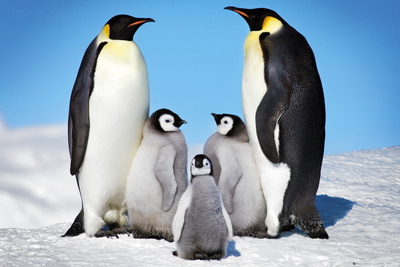
\includegraphics[scale=.50]{figures/Penguins.jpg}
\caption{TAMU figure}
\label{fig:tamu-fig5}
\end{figure}

%%%%%%%%%%%%%%%%%%%%%%%%%%%%%%%%%%%%%%%%%%%%%%%%%%%
%
%  New template code for TAMU Theses and Dissertations starting Fall 2016.
%
%
%  Author: Sean Zachary Roberson 
%	 Version 3.16.09 
%  Last updated 9/12/2016
%
%%%%%%%%%%%%%%%%%%%%%%%%%%%%%%%%%%%%%%%%%%%%%%%%%%%

%%%%%%%%%%%%%%%%%%%%%%%%%%%%%%%%%%%%%%%%%%%%%%%%%%%%%%%%%%%%%%%%%%%%%%
%%                           APPENDIX B
%%%%%%%%%%%%%%%%%%%%%%%%%%%%%%%%%%%%%%%%%%%%%%%%%%%%%%%%%%%%%%%%%%%%%

\chapter{\uppercase {A Second Appendix Whose Title Is Much Longer Than The First}}

Text for the Appendix follows.

\begin{figure}[H]
\centering
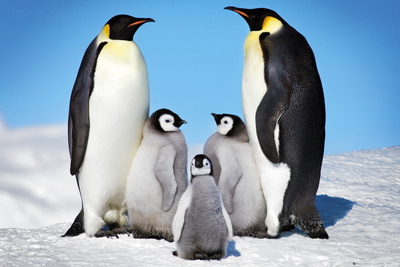
\includegraphics[scale=.50]{figures/Penguins.jpg}
\caption{Another TAMU figure.}
\label{fig:tamu-fig6}
\end{figure}

\section{Appendix Section}

\section{Second Appendix Section}


\pagebreak{}

\end{appendices}


\end{document}
